\documentclass[letterpaper]{report}
\usepackage[text={6.5in,9in},centering]{geometry}
\usepackage[T1]{fontenc}
\usepackage{amssymb}
\usepackage{amsmath}
\usepackage{newpxtext,eulerpx}
\usepackage{sourcecodepro}
\usepackage{listings}
\usepackage{graphicx}
\usepackage{setspace}
\usepackage{tabularx}
\usepackage{longtable}
\pagestyle{plain}
\pagenumbering{arabic}
\usepackage{floatrow}
\usepackage{url}
\usepackage[margin=0.5cm,font=small,format=hang]{caption}
\usepackage[version=4]{mhchem}
\usepackage{color}

\newcommand{\angstrom}{\mbox{\normalfont\AA}}
\let\textDJ\DJ
\let\DJ\relax

\DeclareRobustCommand{\DJ}{%
  \ifmmode
    \mathDJ
  \else
    \textDJ
  \fi
}
\makeatletter
\newcommand{\mathDJ}{\text{\raisebox{0.25ex}{-}\kern-0.4em$\m@th D$}}
\renewcommand{\l@section}{\@dottedtocline{1}{2em}{3em}}
\renewcommand{\l@subsection}{\@dottedtocline{2}{4.0em}{4em}}
\renewcommand{\l@subsubsection}{\@dottedtocline{3}{7.4em}{5em}}
\makeatother

\renewcommand{\baselinestretch}{1.2}
\usepackage[super,comma,sort&compress]{natbib}
\bibpunct{}{}{,}{s}{}{;}
%\bibpunct{[}{]}{,}{n}{}{;}

\DeclareFloatFont{tiny}{\scriptsize}% "scriptsize" is defined by floatrow, "tiny" not
\floatsetup[table]{font=small}

\definecolor{mygreen}{rgb}{0,0.6,0}
\definecolor{mygray}{rgb}{0.5,0.5,0.5}
\definecolor{mymauve}{rgb}{0.58,0,0.82}

%\renewcommand\citemid{\ } % no comma in optional reference note
\lstset{
    language=C,
    frame=TB,
    basicstyle=\footnotesize\ttfamily, %
	xleftmargin=0.25in,
    xrightmargin=0.25in,
    captionpos=b, %
	abovecaptionskip=0.5cm, 
    belowcaptionskip=0.5cm, 
    escapeinside={~}{~},
    identifierstyle=\color{black},
    commentstyle=\color{mygreen}\textit,    % comment style
    keywordstyle=\color{blue},       % keyword style
    stringstyle=\color{mymauve}    % string literal style
}
\renewcommand{\lstlistingname}{Example}

\lstnewenvironment{code}[1][]%
  {\noindent\minipage{\linewidth}\vspace{0.5\baselineskip} 
   \lstset{
    language=C,
    basicstyle=\footnotesize\ttfamily,%
    captionpos=b,
    aboveskip=0.5cm,
    belowskip=0.5cm,
    abovecaptionskip=0.5cm,
    belowcaptionskip=0.5cm,
    escapeinside={~}{~},
    identifierstyle=\color{black},
    commentstyle=\color{mygreen}\textit,    % comment style
    keywordstyle=\color{blue},       % keyword style
    stringstyle=\color{mymauve},     % string literal style
    frame=single,#1}}
{\endminipage}



\begin{document}

\newcolumntype{A}{p{1.5in}}
\newcolumntype{B}{p{0.75in}}
\newcolumntype{C}{p{1.5in}}
\newcolumntype{D}{p{2in}}

\newcolumntype{E}{p{0.25in}}
\newcolumntype{F}{p{2in}}
\newcolumntype{G}{p{3.75in}}

\newcolumntype{H}{p{0.75in}}
\newcolumntype{I}{p{5in}}

\newcolumntype{J}{p{1.5in}}
\newcolumntype{K}{p{0.75in}}
\newcolumntype{L}{p{1.5in}}
\newcolumntype{M}{p{2in}}


\title{OpenMD-3.1: Molecular Dynamics in the Open}

\author{C.R. Drisko, Sydney A. Shavalier,  Benjamin M. Harless, Veronica Freund, \\
  Teng Lin,  Charles F. Vardeman II, Christopher J. Fennell, Matthew  A. Meineke, \\
  Patrick B. Louden,   Hemanta Bhattarai, Joseph R. Michalka, Kelsey M. Stocker, \\
  James M. Marr,  Anderson D.S. Duraes, Suzanne M. Neidhart, Shenyu Kuang,  \\
  Madan Lamichhane, Xiuquan Sun, Chunlei Li, Kyle Daily, \\
  Alexander Mazanek,  Yang Zheng, \\ and \\
  J. Daniel Gezelter \\ \\
  Department of Chemistry and Biochemistry\\
  University of Notre Dame\\
  Notre Dame, Indiana 46556}

\maketitle

\section*{Preface} 

OpenMD is an open source molecular dynamics engine which is
capable of efficiently simulating liquids, proteins, nanoparticles,
interfaces, metals, and other complex systems using atom types with
orientational degrees of freedom (e.g. ``sticky'' atoms, point
multipoles, and coarse-grained assemblies). It is a test-bed for new
molecular simulation methodology, but is also efficient and easy to
use.  Liquids, proteins, zeolites, lipids, inorganic nanomaterials,
transition metals (bulk, flat interfaces, and nanoparticles) and a
wide array of other systems have all been simulated using this
code. OpenMD works on parallel computers using the Message
Passing Interface (MPI), and comes with a number of trajectory
analysis and utility programs that are easy to use and modify. An
OpenMD simulation is specified using a very simple meta-data language
that is easy to learn.

\tableofcontents

%\listoffigures
%\listoftables
%\mainmatter

\chapter{\label{sec:intro}Introduction}

There are a number of excellent molecular dynamics packages available
to the chemical physics
community.\cite{Brooks83,MacKerell98,pearlman:1995,Gromacs,Gromacs3,DL_POLY,Tinker,Paradyn,namd,macromodel}
All of these packages are stable, polished programs which solve many
problems of interest.  Most are now capable of performing molecular
dynamics simulations on parallel computers.  Some have source code
which is freely available to the entire scientific community.  Few,
however, are capable of efficiently integrating the equations of
motion for atom types with orientational degrees of freedom
(e.g. point multipoles, and ``sticky'' atoms).  And only one of the
programs referenced can handle transition metal force fields like the
Embedded Atom Method (EAM).  The direction our research program
has taken us now involves the use of atoms with orientational degrees
of freedom as well as transition metals.  Since these simulation
methods may be of some use to other researchers, we have decided to
release our program (and all related source code) to the scientific
community.

This document communicates the algorithmic details of our program,
OpenMD.  We have structured this document to first discuss the
underlying concepts in this simulation package (Chapter
\ref{section:IOfiles}).  The empirical energy functions implemented
are discussed in Chapter~\ref{chapter:forceFields}.
Section~\ref{section:mechanics} describes the various Molecular Dynamics
algorithms OpenMD implements in the integration of Hamilton's
equations of motion.  Program design considerations for parallel
computing are presented in Sec.~\ref{section:parallelization}.
Concluding remarks are presented in Sec.~\ref{section:conclusion}.

\chapter{\label{section:IOfiles}Concepts \& Files}

A simulation in OpenMD is built using a few fundamental
conceptual building blocks, most of which are chemically intuitive.
The basic unit of a simulation is an {\tt atom}.  The parameters
describing an {\tt atom} have been generalized to make it as flexible
as possible; this means that in addition to translational degrees of
freedom, {\tt atoms} may also have {\it orientational} degrees of
freedom.

The fundamental (static) properties of {\tt atoms} are defined by the
{\tt forceField} chosen for the simulation.  The atomic properties
specified by a {\tt forceField} might include (but are not limited to)
charge, $\sigma$ and $\epsilon$ values for Lennard-Jones interactions,
the strength of the dipole moment ($\mu$), the mass, and the moments
of inertia.  Other more complicated properties of atoms might also be
specified by the {\tt forceField}.

{\tt Atoms} can be grouped together in many ways.  A {\tt rigidBody}
contains atoms that exert no forces on one another and which move as a
single rigid unit.  A {\tt cutoffGroup} may contain atoms which
function together as a (rigid {\it or} non-rigid) unit for potential
energy calculations,
\begin{equation}
V_{ab} = s(r_{ab}) \sum_{i \in a} \sum_{j \in b} V_{ij}(r_{ij})
\end{equation}
Here, $a$ and $b$ are two {\tt cutoffGroups} containing multiple atoms
($a = \left\{i\right\}$ and $b = \left\{j\right\}$).  $s(r_{ab})$ is a
generalized switching function which insures that the atoms in the two
{\tt cutoffGroups} are treated identically as the two groups enter or
leave an interaction region.

{\tt Atoms} may also be grouped in more traditional ways into {\tt
  bonds}, {\tt bends}, {\tt torsions}, and {\tt inversions}.  These
groupings allow the correct choice of interaction parameters for
short-range interactions to be chosen from the definitions in the {\tt
  forceField}.

All of these groups of {\tt atoms} are brought together in the {\tt
molecule}, which is the fundamental structure for setting up an
OpenMD simulation.  {\tt Molecules} contain lists of {\tt atoms}
followed by listings of the other atomic groupings ({\tt bonds}, {\tt
bends}, {\tt torsions}, {\tt rigidBodies}, and {\tt cutoffGroups})
which relate the atoms to one another.  Since a {\tt rigidBody} is a
collection of atoms that are propagated in fixed relationships to one
another, OpenMD uses an internal structure called a {\tt
StuntDouble} to store information about those objects that can change
position {\it independently} during a simulation.  That is, an atom
that is part of a rigid body is not itself a StuntDouble.  In this
case, the rigid body is the StuntDouble.  However, an atom that is
free to move independently {\it is} its own StuntDouble.

Simulations often involve heterogeneous collections of molecules.  To
specify a mixture of {\tt molecule} types, OpenMD uses {\tt
components}.  Even simulations containing only one type of molecule
must specify a single {\tt component}.

Starting a simulation requires two types of information: {\it
meta-data}, which describes the types of objects present in the
simulation, and {\it configuration} information, which describes the
initial state of these objects.  An OpenMD file is a single
combined file format that describes both of these kinds of data.  An
OpenMD file contains one {\tt <MetaData>} block and {\it at least
one} {\tt <Snapshot>} block.

The language for the {\tt <MetaData>} block is a C-based syntax that
is parsed at the beginning of the simulation.  Configuration
information is specified for all {\tt integrableObjects} in a {\tt
<Snapshot>} block.  Both the {\tt <MetaData>} and {\tt <Snapshot>}
formats are described in the following sections.

\begin{code}[caption={[The structure of an OpenMD file]
The basic structure of an OpenMD file contains HTML-like tags to
define simulation meta-data and subsequent instantaneous configuration
information. A well-formed OpenMD file must contain one {\tt <MetaData>}
block and {\it at least one} {\tt <Snapshot>} block.  Each
{\tt <Snapshot>} is further divided into {\tt <FrameData>} and 
 {\tt <StuntDoubles>} sections.},label={sch:mdFormat}]
<OpenMD>
  <MetaData>
      // see section ~\ref{sec:miscConcepts}~ for details on the formatting
      // of information contained inside the <MetaData> tags
  </MetaData>
  <Snapshot>         // An instantaneous configuration
     <FrameData>
                     // FrameData contains information on the time
                     // stamp, the size of the simulation box, and 
                     // the current state of extended system 
                     // ensemble variables.
     </FrameData>
     <StuntDoubles>
                     // StuntDouble information comprises the 
                     // positions, velocities, orientations, and 
                     // angular velocities of anything that is 
                     // capable of independent motion during 
                     // the simulation.
     </StuntDoubles>
     <SiteData>
                    // SiteData displays atomic-level details
                    // of dynamic quantities, e.g. fluctuating charges,
                    // electric fields, etc., computed during a
                    // simulation. This block is not always present.
     </SiteData>
  </Snapshot>       
  <Snapshot>         // Multiple <Snapshot> sections can be
  </Snapshot>        // present in a well-formed OpenMD file
  <Snapshot>         // Further information on <Snapshot> blocks
  </Snapshot>        // can be found in section ~\ref{section:coordFiles}~.
</OpenMD>
\end{code}


\section{OpenMD Files and {\tt <MetaData>} blocks}

OpenMD uses HTML-like delimiters to separate {\tt
  <MetaData>} and {\tt <Snapshot>} blocks.  A C-based syntax
is used to parse the {\tt <MetaData>} blocks at run time.  These
blocks allow the user to completely describe the system they wish to
simulate, as well as tailor OpenMD's behavior during the
simulation.  OpenMD files are typically denoted with the
extension {\tt .omd}. An overview of an OpenMD file is shown in
Example~\ref{sch:mdFormat} and example file is shown in
Example~\ref{sch:mdExample}.

\begin{code}[caption={[An example of a complete OpenMD
file] An example showing a complete OpenMD file.},
label={sch:mdExample}] 
<OpenMD>
  <MetaData>
molecule{
  name = "Ar";
  atom[0]{
    type="Ar";
    position( 0.0, 0.0, 0.0 );
  }
}

component{
  type = "Ar";
  nMol = 3;
}

forceField = "LJ";
ensemble = "NVE"; // specify the simulation ensemble
dt = 1.0;         // the time step for integration
runTime = 1e3;    // the total simulation run time
sampleTime = 100; // trajectory file frequency
statusTime = 50;  // statistics file frequency
  </MetaData>
  <Snapshot>
    <FrameData>
        Time: 0
        Hmat: {{ 28.569, 0, 0 }, { 0, 28.569, 0 }, { 0, 0, 28.569 }}
  Thermostat: 0 , 0
    Barostat: {{ 0, 0, 0 }, { 0, 0, 0 }, { 0, 0, 0 }}
    </FrameData>
    <StuntDoubles>
         0      pv   17.5  13.3 12.8  1.181e-03 -1.630e-03 -1.369e-03
         1      pv  -12.8 -14.9 -8.4 -4.440e-04 -2.048e-03  1.130e-03
         2      pv  -10.0 -15.2 -6.5  2.239e-03 -6.310e-03  1.810e-03
    </StuntDoubles>
  </Snapshot>
</OpenMD>
\end{code}

In the {\tt <MetaData>} block, it is necessary to provide a
complete description of the molecule before it is actually placed in
the simulation. OpenMD's meta-data syntax allows for the use of
{\it include files} to specify all atoms in a molecular prototype, as
well as any bonds, bends, torsions, or other structural groupings of
atoms.  Include files allow the user to describe a molecular prototype
once, then simply include it into each simulation containing that
molecule. Returning to the example in Scheme~\ref{sch:mdExample}, the
include file's contents would be Scheme~\ref{sch:mdIncludeExample},
and the new OpenMD file would become Scheme~\ref{sch:mdExPrime}.

\begin{code}[caption={An example molecule definition in an
include file.},label={sch:mdIncludeExample}]
molecule{
  name = "Ar";
  atom[0]{
    type="Ar";
    position( 0.0, 0.0, 0.0 );
  }
}
\end{code}

\begin{code}[caption={Revised OpenMD input file
example.},label={sch:mdExPrime}]
<OpenMD>
  <MetaData>
#include "argon.inc"

component{
  type = "Ar";
  nMol = 3;
}

forceField = "LJ";
ensemble = "NVE";
dt = 1.0;
runTime = 1e3;
sampleTime = 100;
statusTime = 50; 
  </MetaData>
  </MetaData>
  <Snapshot>
    <FrameData>
        Time: 0
        Hmat: {{ 28.569, 0, 0 }, { 0, 28.569, 0 }, { 0, 0, 28.569 }}
  Thermostat: 0 , 0
    Barostat: {{ 0, 0, 0 }, { 0, 0, 0 }, { 0, 0, 0 }}
    </FrameData>
    <StuntDoubles>
         0      pv   17.5  13.3 12.8  1.181e-03 -1.630e-03 -1.369e-03
         1      pv  -12.8 -14.9 -8.4 -4.440e-04 -2.048e-03  1.130e-03
         2      pv  -10.0 -15.2 -6.5  2.239e-03 -6.310e-03  1.810e-03
    </StuntDoubles>
  </Snapshot>
</OpenMD>
\end{code}

\section{\label{section:atomsMolecules}Atoms, Molecules, and other
ways of grouping atoms}

As mentioned above, the fundamental unit for an OpenMD
simulation is the {\tt atom}.  Atoms can be collected into secondary
structures such as {\tt rigidBodies}, {\tt cutoffGroups}, or {\tt
  molecules}. The {\tt molecule} is a way for OpenMD to keep
track of the atoms in a simulation in logical manner. Molecular units
store the identities of all the atoms and rigid bodies associated with
themselves, and they are responsible for the evaluation of their own
internal interactions (\emph{i.e.}~bonds, bends, torsions, and
inversions). Scheme \ref{sch:mdIncludeExample} shows how one creates a
molecule in an included meta-data file. The positions of the atoms
given in the declaration are relative to the origin of the molecule,
and the origin is used when creating a system containing the molecule.

One of the features that sets OpenMD apart from most of the
current molecular simulation packages is the ability to handle rigid
body dynamics. Rigid bodies are non-spherical particles or collections
of particles (e.g. a phenyl ring) that have a constant internal
potential and move collectively.\cite{Goldstein01} They are not
included in most simulation packages because of the algorithmic
complexity involved in propagating orientational degrees of freedom.
Integrators which propagate orientational motion with an acceptable
level of energy conservation for molecular dynamics are relatively new
inventions.

Moving a rigid body involves determination of both the force and
torque applied by the surroundings, which directly affect the
translational and rotational motion in turn. In order to accumulate
the total force on a rigid body, the external forces and torques must
first be calculated for all the internal particles. The total force on
the rigid body is simply the sum of these external forces.
Accumulation of the total torque on the rigid body is more complex
than the force because the torque is applied to the center of mass of
the rigid body. The space-fixed torque on rigid body $i$ is
\begin{equation}
\boldsymbol{\tau}_i=
	\sum_{a}\biggl[(\mathbf{r}_{ia}-\mathbf{r}_i)\times \mathbf{f}_{ia} 
	+ \boldsymbol{\tau}_{ia}\biggr],
\label{eq:torqueAccumulate}
\end{equation}
where $\boldsymbol{\tau}_i$ and $\mathbf{r}_i$ are the torque on and
position of the center of mass respectively, while $\mathbf{f}_{ia}$,
$\mathbf{r}_{ia}$, and $\boldsymbol{\tau}_{ia}$ are the force on,
position of, and torque on the component particles of the rigid body.

The summation of the total torque is done in the body fixed axis of
each rigid body. In order to move between the space fixed and body
fixed coordinate axes, parameters describing the orientation must be
maintained for each rigid body. At a minimum, the rotation matrix
($\mathsf{A}$) can be described by the three Euler angles ($\phi,
\theta,$ and $\psi$), where the elements of $\mathsf{A}$ are composed of
trigonometric operations involving $\phi, \theta,$ and
$\psi$.\cite{Goldstein01} In order to avoid numerical instabilities
inherent in using the Euler angles, the four parameter ``quaternion''
scheme is often used. The elements of $\mathsf{A}$ can be expressed as
arithmetic operations involving the four quaternions ($q_w, q_x, q_y,$
and $q_z$).\cite{Allen87} Use of quaternions also leads to
performance enhancements, particularly for very small
systems.\cite{Evans77}

Rather than use one of the previously stated methods, OpenMD
utilizes a relatively new scheme that propagates the entire nine
parameter rotation matrix. Further discussion on this choice can be
found in Sec.~\ref{section:integrate}. An example definition of a
rigid body can be seen in Scheme
\ref{sch:rigidBody}.

\begin{code}[caption={[Defining rigid bodies]A sample
definition of a molecule containing a rigid body and a cutoff
group},label={sch:rigidBody}] 
molecule{
  name = "TIP3P";
  atom[0]{
    type = "O_TIP3P";
    position( 0.0, 0.0, -0.06556 );
  }
  atom[1]{
    type = "H_TIP3P";
    position( 0.0, 0.75695, 0.52032 );
  }
  atom[2]{
    type = "H_TIP3P";
    position( 0.0, -0.75695, 0.52032 );
  }

  rigidBody[0]{
    members(0, 1, 2);
  }

  cutoffGroup{
    members(0, 1, 2);
  }
}
\end{code}

\section{\label{sec:miscConcepts}Creating a {\tt <MetaData>} block}

The actual creation of a {\tt <MetaData>} block requires several key
components. The first part of the file needs to be the declaration of
all of the molecule prototypes used in the simulation. This is
typically done through included prototype files. Only the molecules
actually present in the simulation need to be declared; however,
OpenMD allows for the declaration of more molecules than are
needed. This gives the user the ability to build up a library of
commonly used molecules into a single include file.

Once all prototypes are declared, the ordering of the rest of the
block is less stringent.  The molecular composition of the simulation
is specified with {\tt component} statements. Each different type of
molecule present in the simulation is considered a separate
component (an example is shown in
Sch.~\ref{sch:mdExPrime}).  The component blocks tell OpenMD the
number of molecules that will be in the simulation, and the order in
which the components blocks are declared sets the ordering of the real
atoms in the {\tt <Snapshot>} block as well as in the output files. The
remainder of the script then sets the various simulation parameters
for the system of interest.

The required set of parameters that must be present in all simulations
is given in Table~\ref{table:reqParams}.  Since the user can use 
OpenMD to perform energy minimizations as well as molecular
dynamics simulations, either a {\tt minimizer} block or the {\tt
  ensemble} keyword must be present.  The {\tt ensemble} keyword is
responsible for selecting the integration method used for the
calculation of the equations of motion. An in depth discussion of the
various methods available in OpenMD can be found in
Sec.~\ref{section:mechanics}.  The {\tt minimizer} block selects which
minimization method to use, and more details on the choices of
minimizer parameters can be found in Sec.~\ref{section:minimizer}. The
{\tt forceField} statement is important for the selection of which
forces will be used in the course of the simulation. OpenMD
supports several force fields, and allows the user to create their own
using a range of pre-defined empirical energy functions.  The format
of force field files is outlined
Chapter~\ref{chapter:forceFields}. The force fields are
interchangeable between simulations, with the only requirement being
that all atoms needed by the simulation are defined within the
selected force field.

For molecular dynamics simulations, the time step between force
evaluations is set with the {\tt dt} parameter, and {\tt runTime} will
set the time length of the simulation. Note, that {\tt runTime} is an
absolute time, meaning if the simulation is started at t = 10.0~ns
with a {\tt runTime} of 25.0~ns, the simulation will only run for an
additional 15.0~ns.  

For energy minimizations, it is not necessary to specify {\tt dt} or
{\tt runTime}.

To set the initial positions and velocities of all the integrable
objects in the simulation, OpenMD will use the last good {\tt
<Snapshot>} block that was found in the startup file that it was
called with.  If the {\tt useInitalTime} flag is set to {\tt true},
the time stamp from this snapshot will also set the initial time stamp
for the simulation.  Additional parameters are summarized in
Table~\ref{table:genParams}.

It is important to note the fundamental units in all files which are
read and written by OpenMD.  Energies are in $\mbox{kcal
mol}^{-1}$, distances are in $\mbox{\AA}$, times are in $\mbox{fs}$,
translational velocities are in $\mbox{\AA~fs}^{-1}$, and masses are
in $\mbox{amu}$.  Orientational degrees of freedom are described using
quaternions (unitless, but $q_w^2 + q_x^2 + q_y^2 + q_z^2 = 1$),
body-fixed angular momenta ($\mbox{amu \AA}^{2} \mbox{radians
fs}^{-1}$), and body-fixed moments of inertia ($\mbox{amu \AA}^{2}$). 

\begin{longtable}[c]{ABCD}
\caption{Meta-data Keywords: Required Parameters}
\\
{\bf keyword} & {\bf units} & {\bf use} & {\bf remarks}  \\ \hline
\endhead
\hline
\endfoot
{\tt forceField} & string & Sets the base name for the force field file &
OpenMD appends a {\tt .frc} to the end of this to look for a force
field file.\\
{\tt component} & & Defines the molecular components of the system &
Every {\tt <MetaData>} block must have a component statement. \\
{\tt minimizer} & block & Sets parameters for the minimizer & Either {\tt ensemble} or {\tt minimizer} must be specified. \\
{\tt ensemble} & string & Sets the ensemble. & Some possible ensembles are
{\tt NVE, NVT, NPTi, NPAT, NPTf, NPTxyz, LD} and {\tt LangevinHull}.  Either {\tt ensemble}
or {\tt minimizer} must be specified. \\
{\tt dt} & fs & Sets the time step. & Selection of {\tt dt} should be
small enough to sample the fastest motion of the simulation. ({\tt
dt} is required for molecular dynamics simulations)\\
{\tt runTime} & fs & Sets the time at which the simulation should
end. & This is an absolute time, and will end the simulation when the
current time meets or exceeds the {\tt runTime}. ({\tt runTime} is
required for molecular dynamics simulations)
\label{table:reqParams}
\end{longtable}

\begin{longtable}[c]{ABCD}
\caption{Meta-data Keywords: Optional Parameters}
\\
{\bf keyword} & {\bf units} & {\bf use} & {\bf remarks}  \\ \hline
\endhead
\hline
\endfoot
{\tt forceFieldVariant} & string & Sets the name of the variant of the
force field.  & EAM has three variants: {\tt u3}, {\tt u6}, and
{\tt VC}. \\
{\tt forceFieldFileName} & string & Overrides the default force field
file name & Each force field has a default file name, and this
parameter can override the default file name for the chosen force
field. \\
{\tt usePeriodicBoundaryConditions} & & & \\
  & logical & Turns periodic boundary conditions on/off. & Default is true. \\
{\tt orthoBoxTolerance} & double & & decides how orthogonal the periodic
box must be before we can use cheaper box calculations \\
{\tt cutoffRadius} & $\mbox{\AA}$ & Manually sets the cutoff radius &
default is set from {\tt cutoffPolicy} \\ 
{\tt skinThickness} & \AA & thickness of the skin for the Verlet
neighbor lists & defaults to 1 \AA \\
{\tt switchingRadius} & $\mbox{\AA}$  & Manually sets the inner radius
for the switching function. & Defaults to 85~\% of the {\tt
cutoffRadius}. \\
{\tt switchingFunctionType} & & & \\
 & string & {\tt cubic} or
{\tt fifth\_order\_polynomial} & Default is {\tt cubic} \\
{\tt useInitialTime} & logical & Sets whether the initial time is
taken from the last {\tt <Snapshot>} in the startup file. & Useful when recovering a simulation from a crashed processor. Default is {\tt false}. \\
{\tt useInitialExtendedSystemState} & & & \\
  & logical & keep the extended
system variables? & Should the extended
variables (the thermostat and barostat) be kept from the {\tt <Snapshot>} block? \\
{\tt sampleTime} & fs & Sets the frequency at which the {\tt .dump} file is written. & Default is set to {\tt runTime}. \\
{\tt resetTime} & fs & Sets the frequency at which the extended system
variables are reset to zero & The default is to never reset these
variables. \\
{\tt statusTime} & fs & Sets the frequency at which the {\tt .stat} file is written. & Default is set to {\tt sampleTime}. \\
{\tt finalConfig} & string & Sets the name of the final output file. & Useful when stringing simulations together. Defaults to the root name of the initial meta-data file but with an {\tt .eor} extension. \\ 
{\tt compressDumpFile} & logical & & should the {\tt .dump} file be
compressed on the fly? \\
{\tt statFileFormat} & string & columns to print in the {\tt .stat}
file where each column is separated by a pipe ($\mid$) symbol. & (The
default is the first eight of these columns in order.)  \\
& \multicolumn{3}{p{4.25in}}{Allowed
column names are: {\tt TIME, TOTAL\_ENERGY, POTENTIAL\_ENERGY, KINETIC\_ENERGY,
TEMPERATURE, PRESSURE, VOLUME, CONSERVED\_QUANTITY, HULLVOLUME, GYRVOLUME, 
TRANSLATIONAL\_KINETIC, ROTATIONAL\_KINETIC,  LONG\_RANGE\_POTENTIAL,
SHORT\_RANGE\_POTENTIAL, VANDERWAALS\_POTENTIAL,
ELECTROSTATIC\_POTENTIAL, METALLIC\_POTENTIAL,
HYDROGEN\_BONDING\_POTENTIAL, RECIPROCAL\_POTENTIAL,
     SURFACE\_POTENTIAL, BOND\_POTENTIAL, BEND\_POTENTIAL,
DIHEDRAL\_POTENTIAL, INVERSION\_POTENTIAL, RAW\_POTENTIAL, RESTRAINT\_POTENTIAL,
PRESSURE\_TENSOR, SYSTEM\_DIPOLE, SYSTEM\_QUADRUPOLE, HEATFLUX,
ELECTRONIC\_TEMPERATURE, COM, COM\_VELOCITY, ANGULAR\_MOMENTUM, POTENTIAL\_SELECTION }} \\
{\tt printPressureTensor} & logical & sets whether OpenMD will print
out the pressure tensor & can be useful for calculations of the bulk
modulus \\
{\tt electrostaticSummationMethod} & & & \\
 & string & {\tt shifted\_force,
shifted\_potential, hard, switched, taylor\_shifted,} or {\tt reaction\_field} &
default is {\tt shifted\_force} \\
{\tt electrostaticScreeningMethod} & & & \\
 & string & {\tt undamped} or {\tt damped} & default is {\tt damped} \\
{\tt dielectric} & unitless & Sets the dielectric constant for
reaction field. & If {\tt electrostaticSummationMethod} is set to {\tt
reaction\_field}, then {\tt dielectric} must be set. \\
{\tt dampingAlpha} & $\mbox{\AA}^{-1}$ & governs strength of
electrostatic damping & default  = max(0, 0.425 - {\tt cutoffRadius} * 0.02) \\
{\tt tempSet} & logical & resample velocities from a Maxwell-Boltzmann
distribution set to {\tt targetTemp} & default is {\tt false} \\
{\tt thermalTime} & fs & how often to perform a {\tt tempSet} &
default is never \\
{\tt targetTemp} & K & sets the target temperature & no default value \\
{\tt tauThermostat} & fs & time constant for Nos\'{e}-Hoover
thermostat & times from 100-10,000 fs are reasonable \\
{\tt targetPressure} & atm & sets the target pressure & no default value\\
{\tt surfaceTension} &  & sets the target surface tension in the x-y
plane & no default value \\
{\tt tauBarostat} & fs & time constant for the
Nos\'{e}-Hoover-Andersen barostat & times from 1000 to 100,000 fs
are reasonable \\
{\tt seed } & integer & Sets the seed value for the random number generator. & The seed needs to be at least 9 digits long. The default is to take the seed from the CPU clock. \\
\label{table:genParams}
\end{longtable}


\section{\label{section:coordFiles}{\tt <Snapshot>} Blocks}

The standard format for storage of a system's coordinates is the {\tt
<Snapshot>} block , the exact details of which can be seen in
Scheme~\ref{sch:dumpFormat}. As all bonding and molecular information
is stored in the {\tt <MetaData>} blocks, the {\tt <Snapshot>} blocks
contain only the coordinates of the objects which move independently
during the simulation.  It is important to note that {\it not all
atoms} are capable of independent motion.  Atoms which are part of
rigid bodies are not ``integrable objects'' in the equations of
motion; the rigid bodies themselves are the integrable objects.
Therefore, the coordinate file contains coordinates of all the {\tt
integrableObjects} in the system.  For systems without rigid bodies,
this is simply the coordinates of all the atoms.

It is important to note that although the simulation propagates the
complete rotation matrix, directional entities are written out using
quaternions to save space in the output files.

{\tt <Snapshot>} blocks contain an initial sub-block called {\tt
  <FrameData>} which contains the time stamp, the three column vectors
of $\mathsf{H}$, and optional extra information for the extended sytem
ensembles.  Following this, the lines in the {\tt <StuntDoubles>} sub-block provide
information about the instantaneous configuration of each integrable
object.  For each integrable object, the global index is followed by a
short string describing what additional information is present on the
line.  Atoms with only position and velocity information use the {\tt
  pv} string which must then be followed by the position and velocity
vectors for that atom.  Directional atoms and Rigid Bodies typically
use the {\tt pvqj} string which is followed by position, velocity,
quaternions, and lastly, body fixed angular momentum for that
integrable object.

Some {\tt <Snapshot>} blocks may also contain a {\tt <SiteData>} block
that can provide information about fluctuating charge ({\tt c}),
charge velocity ({\tt w}), electric field ({\tt e}) or other data at
atomic sites (with two indices) or at the centers of mass of rigid
bodies (with one index). The {\tt <SiteData>} block is usually not
needed to initiate a simulation, but are often necessary for obtaining
detailed atomic-level information following a simulation.

\begin{code}[caption={[The format of the {\tt <Snapshot>} block]
An example of the format of the {\tt <Snapshot>} block.  There is an
initial sub-block called {\tt <FrameData>} which contains the time
stamp, the three column vectors of $\mathsf{H}$, and optional extra
information for the extended sytem ensembles.  The lines in the {\tt
<StuntDoubles>} sub-block provide information about the instantaneous
configuration of each integrable object.  For each integrable object,
the global index is followed by a short string describing what
additional information is present on the line.  Atoms with only
position and velocity information use the {\tt pv} string which must
then be followed by the position and velocity vectors for that atom.
Directional atoms and Rigid Bodies typically use the {\tt pvqj} string
which is followed by position, velocity, quaternions, and
lastly, body fixed angular momentum for that integrable object.
Some files will also contain a {\tt <SiteData>} block that can provide
additional atomic-level information.},label={sch:dumpFormat}]
  <Snapshot>
    <FrameData>
        Time: 0
        Hmat: {{ Hxx, Hyx, Hzx }, { Hxy, Hyy, Hzy }, { Hxz, Hyz, Hzz }}
  Thermostat: 0 , 0
    Barostat: {{ 0, 0, 0 }, { 0, 0, 0 }, { 0, 0, 0 }}
    </FrameData>
    <StuntDoubles>
         0      pv          x y z vx vy vz
         1      pv          x y z vx vy vz
         2      pvqj        x y z vx vy vz  qw qx qy qz jx jy jz
         3      pvqj        x y z vx vy vz  qw qx qy qz jx jy jz
    </StuntDoubles>
    <SiteData>
         0  0   cwe         c w ex ey ez
         1  0   cwe         c w ex ey ez
         2      cwe         c w ex ey ez
         2  0   cwe         c w ex ey ez
         2  1   cwe         c w ex ey ez
         2  2   cwe         c w ex ey ez
         3      cwe         c w ex ey ez
         3  0   cwe         c w ex ey ez
         3  1   cwe         c w ex ey ez
         3  2   cwe         c w ex ey ez
    </SiteData>         
  </Snapshot>
\end{code}

There are three OpenMD files that are written using the combined
format.  They are: the initial startup file (\texttt{.omd}), the
simulation trajectory file (\texttt{.dump}), and the final coordinates
or ``end-of-run'' for the simulation (\texttt{.eor}). The initial
startup file is necessary for OpenMD to start the simulation with
the proper coordinates, and this file must be generated by the user
before the simulation run. The trajectory (or ``dump'') file is
updated during simulation and is used to store snapshots of the
coordinates at regular intervals. The first frame is a duplication of
the initial configuration (the last good {\tt <Snapshot>} in the
startup file), and each subsequent frame is appended to the dump file
at an interval specified in the meta-data file with the
\texttt{sampleTime} flag. The final coordinate file is the
``end-of-run'' file.  The \texttt{.eor} file stores the final
configuration of the system for a given simulation. The file is
updated at the same time as the \texttt{.dump} file, but it only
contains the most recent frame. In this way, an \texttt{.eor} file may
be used to initialize a second simulation should it be necessary to
recover from a crash or power outage. The coordinate files generated
by OpenMD (both \texttt{.dump} and \texttt{.eor}) all contain the
same {\tt <MetaData>} block as the startup file, so they may be
used to start up a new simulation if desired.

\section{\label{section:initCoords}Generation of Initial Coordinates}

As was stated in Sec.~\ref{section:coordFiles}, a meaningful {\tt
<Snapshot>} block is necessary for specifying for the starting
coordinates for a simulation.  Since each simulation is different,
system creation is left to the end user; however, we have included a
few sample programs which make some specialized structures.  The {\tt
<Snapshot>} block must index the integrable objects in the correct
order.  The ordering of the integrable objects relies on the ordering
of molecules within the {\tt <MetaData>} block. OpenMD
expects the order to comply with the following guidelines:
\begin{enumerate}
\item All of the molecules of the first declared component are given
before proceeding to the molecules of the second component, and so on
for all subsequently declared components.
\item The ordering of the atoms for each molecule follows the order
declared in the molecule's declaration within the model file.
\item Only atoms which are not members of a {\tt rigidBody} are
included.
\item Rigid Body coordinates for a molecule are listed immediately
after the the other atoms in a molecule.  Some molecules may be
entirely rigid, in which case, only the rigid body coordinates are
given.
\end{enumerate}
An example is given in the OpenMD file in Scheme~\ref{sch:initEx1}.

\begin{code}[caption={Example declaration of the
$\text{I}_2$ molecule and the HCl molecule in {\tt <MetaData>} and
{\tt <Snapshot>} blocks.  Note that even though $\text{I}_2$ is
declared before HCl, the {\tt <Snapshot>} block follows the order {\it in
which the components were included}.}, label=sch:initEx1] 
<OpenMD>
  <MetaData>
molecule{
  name = "I2";
  atom[0]{ type = "I"; }
  atom[1]{ type = "I"; }
  bond{ members( 0, 1); }
}
molecule{
  name = "HCl"
  atom[0]{ type = "H";}
  atom[1]{ type = "Cl";}
  bond{ members( 0, 1); }
}
component{
  type = "HCl";
  nMol = 4;
}
component{
  type = "I2";
  nMol = 1;
}
  </MetaData>
  <Snapshot>
    <FrameData>
        Time: 0
        Hmat: {{ 10.0, 0.0, 0.0 }, { 0.0, 10.0, 0.0 }, { 0.0, 0.0, 10.0 }}
    </FrameData>
    <StuntDoubles>
         0      pv          x y z vx vy vz // H from first HCl molecule 
         1      pv          x y z vx vy vz // Cl from first HCl molecule
         2      pv          x y z vx vy vz // H from second HCl molecule 
         3      pv          x y z vx vy vz // Cl from second HCl molecule
         4      pv          x y z vx vy vz // H from third HCl molecule 
         5      pv          x y z vx vy vz // Cl from third HCl molecule
         6      pv          x y z vx vy vz // H from fourth HCl molecule 
         7      pv          x y z vx vy vz // Cl from fourth HCl molecule
         8      pv          x y z vx vy vz // First I from I2 molecule
         9      pv          x y z vx vy vz // Second I from I2 molecule
    </StuntDoubles>
  </Snapshot>
</OpenMD>
\end{code}

\section{The Statistics ({\tt .stat}) and Report ({\tt .report}) Files}

An important output file generated by OpenMD is the statistics
file. This file records such statistical quantities as the
instantaneous temperature (in $K$), volume (in $\mbox{\AA}^{3}$),
pressure (in $\mbox{atm}$), etc. It is written out with the frequency
specified in the meta-data file with the
\texttt{statusTime} keyword. The file allows the user to observe the
system variables as a function of simulation time while the simulation
is in progress. One useful function the statistics file serves is to
monitor the conserved quantity of a given simulation ensemble,
allowing the user to gauge the stability of the integrator. The
statistics file is denoted with the \texttt{.stat} file extension.
The fields printed in the {\tt .stat} file are determined by the {\tt
  statFileFormat} keyword that the user sets in the {\tt <MetaData>} block.

At the end of a simulation, OpenMD will also produce a {\tt
  .report} file. This file contain statistical means and 95\%
confidence intervals for the fields printed in the {\tt .stat} file.
Report files can be very useful in determining how to alter the
simulation box to set an average volume after a constant pressure
simulation, and for verifying that the energy or conserved quantity
has been conserved reasonably well during a simulation.

\chapter{\label{chapter:forceFields}Force Fields}

Like many molecular simulation packages, OpenMD splits the
potential energy into the short-ranged (bonded) portion and a
long-range (non-bonded) potential,
\begin{equation}
V = V_{\mathrm{short-range}} + V_{\mathrm{long-range}}.
\end{equation}
The short-ranged portion includes the bonds, bends, torsions, and
inversions which have been defined in the meta-data file for the
molecules.  The functional forms and parameters for these interactions
are defined by the force field which is selected in the MetaData
section.

\section{\label{section:divisionOfLabor}Separation into Internal and
  Cross interactions}

The classical potential energy function for a system composed of $N$
molecules is traditionally written
\begin{equation}
V = \sum^{N}_{I=1} V^{I}_{\text{Internal}}
	+ \sum^{N-1}_{I=1} \sum_{J>I} V^{IJ}_{\text{Cross}},
\label{eq:totalPotential}
\end{equation}
where $V^{I}_{\text{Internal}}$ contains all of the terms internal to
molecule $I$ (e.g. bonding, bending, torsional, and inversion terms)
and $V^{IJ}_{\text{Cross}}$ contains all intermolecular interactions
between molecules $I$ and $J$.  For large molecules, the internal
potential may also include some non-bonded terms like electrostatic or
van der Waals interactions.

The types of atoms being simulated, as well as the specific functional
forms and parameters of the intra-molecular functions and the
long-range potentials are defined by the force field. In the following
sections we discuss the stucture of an OpenMD force field file and the
specification of blocks that may be present within these files.

\section{\label{section:frcFile}Force Field Files}

Force field files have a number of ``Blocks'' to delineate different
types of information.  The blocks contain AtomType data, which provide
properties belonging to a single AtomType, as well as interaction
information which provides information about bonded or non-bonded
interactions that cannot be deduced from AtomType information alone.
A simple example of a forceField file is shown in scheme
\ref{sch:frcExample}.

\begin{code}[caption={[An example of a complete OpenMD
 force field file for straight-chain united-atom alkanes.] An example
 showing a complete OpenMD force field for straight-chain united-atom
 alkanes.}, label={sch:frcExample}] 
begin Options 
  Name = "alkane" 
end Options

begin BaseAtomTypes  
//name          mass  
C               12.0107
end BaseAtomTypes

begin AtomTypes
//name  base    mass
CH4	C	16.05		
CH3	C	15.04		
CH2	C	14.03		
end AtomTypes

begin LennardJonesAtomTypes
//name          epsilon         sigma
CH4       	0.2941          3.73
CH3       	0.1947          3.75
CH2       	0.09140         3.95
end LennardJonesAtomTypes

begin BondTypes
//AT1       AT2 Type                    r0              k
CH3	    CH3	Harmonic		1.526		260
CH3	    CH2	Harmonic		1.526		260
CH2	    CH2	Harmonic		1.526		260
end BondTypes

begin BendTypes
//AT1   AT2     AT3     Type            theta0   k
CH3     CH2     CH3     Harmonic        114.0    124.19
CH3     CH2     CH2     Harmonic        114.0    124.19
CH2     CH2     CH2     Harmonic        114.0    124.19
end BendTypes

begin TorsionTypes
//AT1 AT2  AT3  AT4  Type    
CH3   CH2  CH2  CH3  Trappe  0.0  0.70544  -0.13549  1.5723
CH3   CH2  CH2  CH2  Trappe  0.0  0.70544  -0.13549  1.5723  
CH2   CH2  CH2  CH2  Trappe  0.0  0.70544  -0.13549  1.5723  
end TorsionTypes
\end{code}

\section{\label{section:ffOptions}The {\tt Options} block}

The Options block defines properties governing how the force field
interactions are carried out.  This block is delineated with the text
tags {\tt begin Options} and {\tt end Options}.  Most options don't
need to be set as they come with fairly sensible default values, but
the various keywords and their possible values are given in Scheme
\ref{sch:optionsBlock}. 

\begin{code}[caption={[A force field Options block showing default values
for many force field options.] A force field Options block showing default values
for many force field options.  Most of these options do not need to be
specified if the default values are working.},
label={sch:optionsBlock}] 
begin Options
 Name                      "alkane"       // any string
 vdWtype                   "Lennard-Jones" 
 DistanceMixingRule        "arithmetic"   // can also be "geometric" or "cubic"
 DistanceType              "sigma"        // can also be "Rmin"
 EnergyMixingRule          "geometric"    // can also be "arithmetic" or "hhg"
 EnergyUnitScaling         1.0            // multipliers required to get to kcal / mol
 MetallicEnergyUnitScaling 1.0            
 FluctuatingChargeEnergyUnitScaling  1.0
 DistanceUnitScaling       1.0            // multiplier required to get to Angstroms
 AngleUnitScaling          1.0
 ChargeUnitScaling         1.0            // multiplier required to get to electrons
 OxidationStateScaling     1.0
 BondForceConstantScaling  1.0
 BendForceConstantScaling  1.0
 TorsionAngleConvention    "180_is_trans" // can also be "0_is_trans"
 vdW-12-scale              0.0
 vdW-13-scale              0.0
 vdW-14-scale              0.0
 electrostatic-12-scale    0.0
 electrostatic-13-scale    0.0
 electrostatic-14-scale    0.0
 GayBerneMu                2.0
 GayBerneNu                1.0
 EAMMixingMethod           "Johnson"      // can also be "Daw"
end Options
\end{code}

\section{\label{section:ffBase}The {\tt BaseAtomTypes} block}

An {\tt AtomType} is the primary data structure that OpenMD uses to store
static data about an atom.  Things that belong to AtomType are
universal properties (i.e. does this atom have a fixed charge?  What
is its mass?)  Dynamic properties of an atom are not intended to be
properties of an atom type.  A BaseAtomType can be used to build
extended sets of related atom types that all fall back to one
particular type.  For example, one might want a series of atomTypes
that inherit from more basic types:
\begin{displaymath}
\mathtt{ALA-CA} \rightarrow \mathtt{CT} \rightarrow \mathtt{CSP3} \rightarrow \mathtt{C}
\end{displaymath}
where for each step to the right, the atomType falls back to more
primitive data.  That is, the mass could be a property of the {\tt C}
type, while Lennard-Jones parameters could be properties of the {\tt
  CSP3} type.  {\tt CT} could have charge information and its own set
of Lennard-Jones parameter that override the CSP3 parameters.  And the
{\tt ALA-CA} type might have specific torsion or charge information
that override the lower level types.  A BaseAtomType contains only
information a primitive name and the mass of this atom type.
BaseAtomTypes can also be useful in creating files that can be easily
viewed in visualization programs.  The {\tt Dump2XYZ} utility has the
ability to print out the names of the base atom types for displaying
simulations in Jmol or VMD.

\begin{code}[caption={[A simple example of a BaseAtomTypes
block.] A simple example of a BaseAtomTypes block.},
label={sch:baseAtomTypesBlock}] 
begin BaseAtomTypes
//Name  mass (amu)
H       1.0079
O       15.9994
Si      28.0855
Al      26.981538
Mg      24.3050
Ca      40.078
Fe      55.845
Li      6.941
Na      22.98977
K       39.0983
Cs      132.90545
Ca      40.078
Ba      137.327
Cl      35.453
end BaseAtomTypes
\end{code}

\section{\label{section:ffAtom}The {\tt AtomTypes} block}

AtomTypes inherit most properties from BaseAtomTypes, but can override
their lower-level properties as well.  Scheme \ref{sch:atomTypesBlock}
shows an example where multiple types of oxygen atoms can inherit mass
from the oxygen base type.

\begin{code}[caption={[An example of a AtomTypes block.] A
simple example of an AtomTypes block which
shows how multiple types can inherit from the same base type.},
label={sch:atomTypesBlock}]
begin AtomTypes    
//Name  baseatomtype
h*      H
ho      H
o*      O
oh      O
ob      O
obos    O
obts    O
obss    O
ohs     O
st      Si
ao      Al
at      Al
mgo     Mg
mgh     Mg
cao     Ca
cah     Ca
feo     Fe
lio     Li
end AtomTypes
\end{code}

\section{\label{section:ffDirectionalAtom}The {\tt DirectionalAtomTypes}
  block}
DirectionalAtoms have orientational degrees of freedom as well as
translation, so moving these atoms requires information about the
moments of inertias in the same way that translational motion requires
mass.  For DirectionalAtoms, OpenMD treats the mass distribution with
higher priority than electrostatic distributions; the moment of
inertia tensor, $\overleftrightarrow{\mathsf I}$, should be
diagonalized to obtain body-fixed axes, and the three diagonal moments
should correspond to rotational motion \textit{around} each of these
body-fixed axes.  Charge distributions may then result in dipole
vectors that are oriented along a linear combination of the body-axes,
and in quadrupole tensors that are not necessarily diagonal in the
body frame. 

\begin{code}[caption={[An example of a DirectionalAtomTypes block.] A
simple example of a DirectionalAtomTypes block.},
label={sch:datomTypesBlock}]
begin DirectionalAtomTypes
//Name          I_xx    I_yy    I_zz    (All moments in (amu*Ang^2)
SSD             1.7696  0.6145  1.1550  
GBC6H6          88.781  88.781  177.561
GBCH3OH         4.056   20.258  20.999
GBH2O           1.777   0.581   1.196
CO2             43.06   43.06   0.0    // single-site model for CO2
end DirectionalAtomTypes                    

\end{code}

For a DirectionalAtom that represents a linear object, it is
appropriate for one of the moments of inertia to be zero.  In this
case, OpenMD identifies that DirectionalAtom as having only 5 degrees
of freedom (three translations and two rotations), and will alter
calculation of temperatures to reflect this.

\section{\label{section::ffAtomProperties}AtomType properties}
\subsection{\label{section:ffLJ}The {\tt LennardJonesAtomTypes} block}
One of the most basic interatomic interactions implemented in OpenMD
is the Lennard-Jones potential, which mimics the van der
Waals interaction at long distances and uses an empirical repulsion at
short distances. The Lennard-Jones potential is given by:
\begin{equation}
V_{\text{LJ}}(r_{ij}) = 
	4\epsilon_{ij} \biggl[
	\biggl(\frac{\sigma_{ij}}{r_{ij}}\biggr)^{12}
	- \biggl(\frac{\sigma_{ij}}{r_{ij}}\biggr)^{6}
	\biggr],
\label{eq:lennardJonesPot}
\end{equation}
where $r_{ij}$ is the distance between particles $i$ and $j$,
$\sigma_{ij}$ scales the length of the interaction, and
$\epsilon_{ij}$ scales the well depth of the potential.

Interactions between dissimilar particles requires the generation of
cross term parameters for $\sigma$ and $\epsilon$. These parameters
are usually determined using the Lorentz-Berthelot mixing
rules:\cite{Allen87}
\begin{equation}
\sigma_{ij} = \frac{1}{2}[\sigma_{ii} + \sigma_{jj}],
\label{eq:sigmaMix}
\end{equation}
and
\begin{equation}
\epsilon_{ij} = \sqrt{\epsilon_{ii} \epsilon_{jj}}.
\label{eq:epsilonMix}
\end{equation}

The values of $\sigma_{ii}$ and $\epsilon_{ii}$ are properties of atom
type $i$, and must be specified in a section of the force field file
called the {\tt LennardJonesAtomTypes} block (see listing
\ref{sch:LJatomTypesBlock}).  Separate Lennard-Jones interactions
which are not determined by the mixing rules can also be specified in
the {\tt NonbondedInteractionTypes} block (see section
\ref{section:ffNBinteraction}).

\begin{code}[caption={[An example of a LennardJonesAtomTypes block.] A
simple example of a LennardJonesAtomTypee block.   Units for
$\epsilon$ are kcal / mol and for $\sigma$ are \AA\ .},
label={sch:LJatomTypesBlock}]
begin LennardJonesAtomTypes
//Name          epsilon             sigma       
O_TIP4P         0.1550          3.15365 
O_TIP4P-Ew      0.16275         3.16435
O_TIP5P         0.16            3.12   
O_TIP5P-E       0.178           3.097   
O_SPCE          0.15532         3.16549
O_SPC           0.15532         3.16549
CH4             0.279           3.73
CH3             0.185           3.75
CH2             0.0866          3.95
CH              0.0189          4.68
end LennardJonesAtomTypes
\end{code}

\subsection{\label{section:ffCharge}The {\tt ChargeAtomTypes} block}

In molecular simulations, proper accumulation of the electrostatic
interactions is essential and is one of the most
computationally-demanding tasks.  Most common molecular mechanics
force fields represent atomic sites with full or partial charges
protected by Lennard-Jones (short range) interactions.  Partial charge
values, $q_i$ are empirical representations of the distribution of
electronic charge in a molecule.  This means that nearly every pair
interaction involves a calculation of charge-charge forces.  Coupled
with relatively long-ranged $r^{-1}$ decay, the monopole interactions
quickly become the most expensive part of molecular simulations.  The
interactions between point charges can be handled via a number of
different algorithms, but Coulomb's law is the fundamental physical
principle governing these interactions,
\begin{equation}
  V_{\text{charge}}(r_{ij}) = \sum_{ij}\frac{q_iq_je^2}{4 \pi \epsilon_0
    r_{ij}}, 
\end{equation}
where $q$ represents the charge on particle $i$ or $j$, and $e$ is the
charge of an electron in Coulombs.  $\epsilon_0$ is the permittivity
of free space.

\begin{code}[caption={[An example of a ChargeAtomTypes block.] A
simple example of a ChargeAtomTypes block.   Units for
charge are in multiples of electron charge.},
label={sch:ChargeAtomTypesBlock}]
begin ChargeAtomTypes
// Name         charge
O_TIP3P        -0.834
O_SPCE         -0.8476
H_TIP3P         0.417
H_TIP4P         0.520
H_SPCE          0.4238
EP_TIP4P       -1.040
Na+             1.0
Cl-            -1.0
end ChargeAtomTypes
\end{code}

\subsection{\label{section:ffMultipole}The {\tt MultipoleAtomTypes}
  block}
For complex charge distributions that are centered on single sites, it
is convenient to write the total electrostatic potential in terms of
multipole moments,
\begin{equation}
U_{\bf{ab}}(r)=\hat{M}_{\bf a} \hat{M}_{\bf b} \frac{1}{r}  \label{kernel}.
\end{equation}
where the multipole operator on site $\bf a$,
\begin{equation}
\hat{M}_{\bf a} = C_{\bf a} - D_{{\bf a}\alpha} \frac{\partial}{\partial r_{\alpha}} 
+  Q_{{\bf a}\alpha\beta}
 \frac{\partial^2}{\partial r_{\alpha} \partial r_{\beta}} + \dots
\end{equation}
Here, the point charge, dipole, and quadrupole for site $\bf a$ are
given by $C_{\bf a}$, $D_{{\bf a}\alpha}$, and $Q_{{\bf
    a}\alpha\beta}$, respectively.  These are the {\it primitive}
multipoles.  If the site is representing a distribution of charges,
these can be expressed as,
\begin{align}
C_{\bf a} =&\sum_{k \, \text{in \bf a}} q_k , \label{eq:charge} \\
D_{{\bf a}\alpha} =&\sum_{k \, \text{in \bf a}} q_k r_{k\alpha}, \label{eq:dipole}\\
Q_{{\bf a}\alpha\beta} =& \frac{1}{2} \sum_{k \, \text{in \bf a}} q_k
r_{k\alpha}  r_{k\beta} . \label{eq:quadrupole}
\end{align}
Note that the definition of the primitive quadrupole here differs from
the standard traceless form, and contains an additional Taylor-series
based factor of $1/2$.  

The details of the multipolar interactions will be given later, but
many readers are familiar with the dipole-dipole potential:
\begin{equation}
V_{\text{dipole}}(\mathbf{r}_{ij},\boldsymbol{\Omega}_{i},
	\boldsymbol{\Omega}_{j}) = \frac{|{\bf D}_i||{\bf D}_j|}{4\pi\epsilon_{0}r_{ij}^{3}} \biggl[
	\boldsymbol{\hat{u}}_{i} \cdot \boldsymbol{\hat{u}}_{j}
	-
	3(\boldsymbol{\hat{u}}_i \cdot \hat{\mathbf{r}}_{ij}) %
		(\boldsymbol{\hat{u}}_j \cdot \hat{\mathbf{r}}_{ij}) \biggr].
\label{eq:dipolePot}
\end{equation}
Here $\mathbf{r}_{ij}$ is the vector starting at atom $i$ pointing
towards $j$, and $\boldsymbol{\Omega}_i$ and $\boldsymbol{\Omega}_j$
are the orientational degrees of freedom for atoms $i$ and $j$
respectively. The magnitude of the dipole moment of atom $i$ is $|{\bf
  D}_i|$, $\boldsymbol{\hat{u}}_i$ is the standard unit orientation
vector of $\boldsymbol{\Omega}_i$, and $\boldsymbol{\hat{r}}_{ij}$ is
the unit vector pointing along $\mathbf{r}_{ij}$
($\boldsymbol{\hat{r}}_{ij}=\mathbf{r}_{ij}/|\mathbf{r}_{ij}|$).


\begin{code}[caption={[An example of a MultipoleAtomTypes block.] A
simple example of a MultipoleAtomTypes block.   Dipoles are given in
units of Debyes, and Quadrupole moments are given in units of Debye
\AA~(or $10^{-26} \mathrm{~esu~cm}^2$)},
label={sch:MultipoleAtomTypesBlock}]
begin MultipoleAtomTypes
// Euler angles are given in zxz convention in units of degrees.
//
// point dipoles:
// name d phi theta psi dipole_moment
DIP     d 0.0 0.0   0.0     1.91   // dipole points along z-body axis
//
// point quadrupoles:
// name q phi theta psi Qxx Qyy Qzz
CO2     q 0.0 0.0   0.0 0.0 0.0 -0.430592  //quadrupole tensor has zz element
//
// Atoms with both dipole and quadrupole moments:
// name dq phi theta psi dipole_moment  Qxx    Qyy     Qzz
SSD     dq 0.0 0.0   0.0     2.35      -1.682  1.762   -0.08
end MultipoleAtomTypes
\end{code}

Specifying a MultipoleAtomType requires declaring how the
electrostatic frame for the site is rotated relative to the body-fixed
axes for that atom. The Euler angles $(\phi, \theta, \psi)$ for this
rotation must be given, and then the dipole, quadrupole, or all of
these moments are specified in the electrostatic frame.  In OpenMD,
the Euler angles are specified in the $zxz$ convention and are entered
in units of degrees.  Dipole moments are entered in units of Debye,
and Quadrupole moments in units of Debye \AA.

%\subsection{\label{section:ffGB}The FluctuatingChargeAtomTypes  block}
%\subsubsection{\label{section:ffPol}The PolarizableAtomTypes block}

\subsection{\label{section:ffGB}The {\tt GayBerneAtomTypes} block}

The Gay-Berne potential has been widely used in the liquid crystal
community to describe anisotropic phase
behavior.~\cite{Gay:1981yu,Berne:1972pb,Kushick:1976xy,Luckhurst:1990fy,Cleaver:1996rt}
The form of the Gay-Berne potential implemented in OpenMD was
generalized by Cleaver {\it et al.} and is appropriate for dissimilar
uniaxial ellipsoids.\cite{Cleaver:1996rt} The potential is constructed
in the familiar form of the Lennard-Jones function using
orientation-dependent $\sigma$ and $\epsilon$ parameters,
\begin{equation*}
V_{ij}({{\bf \hat u}_i}, {{\bf \hat u}_j}, {{\bf \hat
r}_{ij}}) = 4\epsilon ({{\bf \hat u}_i}, {{\bf \hat u}_j},
{{\bf \hat r}_{ij}})\left[\left(\frac{\sigma_0}{r_{ij}-\sigma({{\bf \hat u
}_i},
{{\bf \hat u}_j}, {{\bf \hat r}_{ij}})+\sigma_0}\right)^{12}
-\left(\frac{\sigma_0}{r_{ij}-\sigma({{\bf \hat u}_i}, {{\bf \hat u}_j},
{{\bf \hat r}_{ij}})+\sigma_0}\right)^6\right]
\label{eq:gb}
\end{equation*}

The range $(\sigma({\bf \hat{u}}_{i},{\bf \hat{u}}_{j},{\bf
\hat{r}}_{ij}))$, and strength $(\epsilon({\bf \hat{u}}_{i},{\bf
\hat{u}}_{j},{\bf \hat{r}}_{ij}))$ parameters 
are dependent on the relative orientations of the two ellipsoids (${\bf
\hat{u}}_{i},{\bf \hat{u}}_{j}$) as well as the direction of the
inter-ellipsoid separation (${\bf \hat{r}}_{ij}$).  The shape and
attractiveness of each ellipsoid is governed by a relatively small set
of parameters: 
\begin{itemize}
\item  $d$:  range parameter for the side-by-side (S) and cross (X) configurations
\item  $l$:  range parameter for the end-to-end (E) configuration
\item  $\epsilon_X$:  well-depth parameter for the cross (X) configuration
\item  $\epsilon_S$:  well-depth parameter for the side-by-side (S) configuration
\item  $\epsilon_E$:  well depth parameter for the end-to-end (E) configuration
\item  $dw$: The ``softness'' of the potential
\end{itemize}
Additionally, there are two universal paramters to govern the overall
importance of the purely orientational ($\nu$) and the mixed
orientational / translational ($\mu$) parts of strength of the
interactions.  These parameters have default or ``canonical'' values,
but may be changed as a force field option:
\begin{itemize}
  \item $\nu$: purely orientational part : defaults to 1
  \item $\mu$: mixed orientational / translational part : defaults to
    2
\end{itemize}
Further details of the potential are given
elsewhere,\cite{Luckhurst:1990fy,Golubkov06,SunX._jp0762020} and an
excellent overview of the computational methods that can be used to
efficiently compute forces and torques for this potential can be found
in Ref. \citenum{Golubkov06}

\begin{code}[caption={[An example of a GayBerneAtomTypes block.] A
simple example of a GayBerneAtomTypes block.  Distances ($d$ and $l$)
are given in \AA\ and energies ($\epsilon_X, \epsilon_S, \epsilon_E$)
are in units of kcal/mol. $dw$ is unitless.},
label={sch:GayBerneAtomTypes}]
begin GayBerneAtomTypes
//Name          d       l       eps_X           eps_S           eps_E     dw
GBlinear        2.8104  9.993   0.774729        0.774729        0.116839  1.0
GBC6H6          4.65    2.03    0.540           0.540           1.9818    0.6
GBCH3OH         2.55    3.18    0.542           0.542           0.55826   1.0
end GayBerneAtomTypes                   
\end{code}

\subsection{\label{section:ffSticky}The {\tt StickyAtomTypes} block}

One of the solvents that can be simulated by OpenMD is the
extended Soft Sticky Dipole (SSD/E) water model.\cite{fennell04} The
original SSD was developed by Ichiye \emph{et
  al.}\cite{liu96:new_model} as a modified form of the hard-sphere
water model proposed by Bratko, Blum, and
Luzar.\cite{Bratko85,Bratko95} It consists of a single point dipole
with a Lennard-Jones core and a sticky potential that directs the
particles to assume the proper hydrogen bond orientation in the first
solvation shell. Thus, the interaction between two SSD water molecules
\emph{i} and \emph{j} is given by the potential
\begin{equation}
V_{ij} = 
	V_{ij}^{LJ} (r_{ij})\ + V_{ij}^{dp}
	(\mathbf{r}_{ij},\mathbf{\Omega}_i,\mathbf{\Omega}_j)\ +
	V_{ij}^{sp}
	(\mathbf{r}_{ij},\mathbf{\Omega}_i,\mathbf{\Omega}_j),
\label{eq:ssdPot}
\end{equation}
where the $\mathbf{r}_{ij}$ is the position vector between molecules
\emph{i} and \emph{j} with magnitude equal to the distance $r_{ij}$, and
$\mathbf{\Omega}_i$ and $\mathbf{\Omega}_j$ represent the
orientations of the respective molecules. The Lennard-Jones and dipole
parts of the potential are given by equations \ref{eq:lennardJonesPot}
and \ref{eq:dipolePot} respectively. The sticky part is described by
the following,
\begin{equation}
u_{ij}^{sp}(\mathbf{r}_{ij},\mathbf{\Omega}_i,\mathbf{\Omega}_j)=
	\frac{\nu_0}{2}[s(r_{ij})w(\mathbf{r}_{ij},
	\mathbf{\Omega}_i,\mathbf{\Omega}_j) +
	s^\prime(r_{ij})w^\prime(\mathbf{r}_{ij},
	\mathbf{\Omega}_i,\mathbf{\Omega}_j)]\ ,
\label{eq:stickyPot}
\end{equation}
where $\nu_0$ is a strength parameter for the sticky potential, and
$s$ and $s^\prime$ are cubic switching functions which turn off the
sticky interaction beyond the first solvation shell. The $w$ function
can be thought of as an attractive potential with tetrahedral
geometry:
\begin{equation}
w(\mathbf{r}_{ij},\mathbf{\Omega}_i,\mathbf{\Omega}_j)=
	\sin\theta_{ij}\sin2\theta_{ij}\cos2\phi_{ij},
\label{eq:stickyW}
\end{equation}
while the $w^\prime$ function counters the normal aligned and
anti-aligned structures favored by point dipoles:
\begin{equation}
w^\prime(\mathbf{r}_{ij},\mathbf{\Omega}_i,\mathbf{\Omega}_j)=
	(\cos\theta_{ij}-0.6)^2(\cos\theta_{ij}+0.8)^2-w^0,
\label{eq:stickyWprime}
\end{equation}
It should be noted that $w$ is proportional to the sum of the $Y_3^2$
and $Y_3^{-2}$ spherical harmonics (a linear combination which
enhances the tetrahedral geometry for hydrogen bonded structures),
while $w^\prime$ is a purely empirical function.  A more detailed
description of the functional parts and variables in this potential
can be found in the original SSD
articles.\cite{liu96:new_model,liu96:monte_carlo,chandra99:ssd_md,Ichiye03}

\begin{figure}
\centering
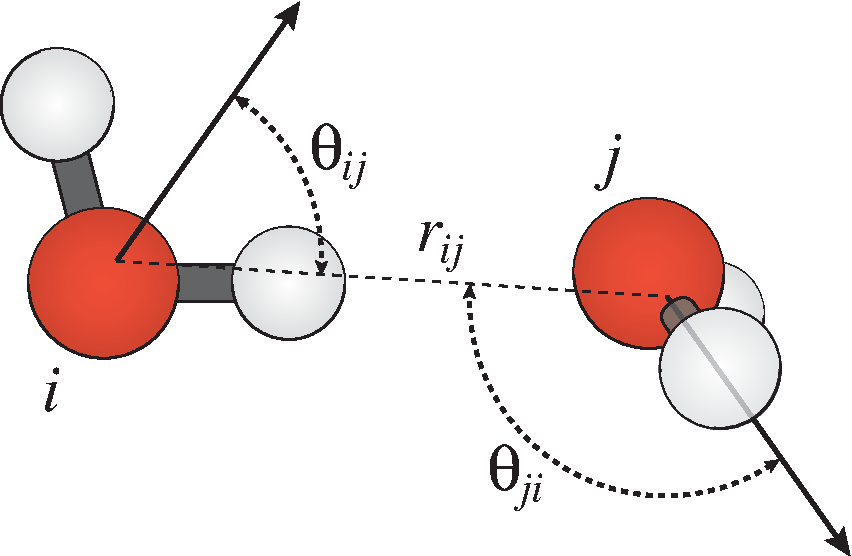
\includegraphics[width=\linewidth]{waterAngle.pdf}
\caption[Coordinate definition for the SSD/E water model]{Coordinates
for the interaction between two SSD/E water molecules.  $\theta_{ij}$
is the angle that $r_{ij}$ makes with the $\hat{z}$ vector in the
body-fixed frame for molecule $i$.  The $\hat{z}$ vector bisects the
HOH angle in each water molecule. } 
\label{fig:ssd}
\end{figure}

Since SSD/E is a single-point {\it dipolar} model, the force
calculations are simplified significantly relative to the standard
{\it charged} multi-point models. In the original Monte Carlo
simulations using this model, Ichiye {\it et al.} reported that using
SSD decreased computer time by a factor of 6-7 compared to other
models.\cite{liu96:new_model} What is most impressive is that these
savings did not come at the expense of accurate depiction of the
liquid state properties.  Indeed, SSD/E maintains reasonable agreement
with the Head-Gordon diffraction data for the structural features of
liquid water.\cite{hura00,liu96:new_model} Additionally, the dynamical
properties exhibited by SSD/E agree with experiment better than those
of more computationally expensive models (like TIP3P and
SPC/E).\cite{chandra99:ssd_md} The combination of speed and accurate
depiction of solvent properties makes SSD/E a very attractive model
for the simulation of large scale biochemical simulations.

Recent constant pressure simulations revealed issues in the original
SSD model that led to lower than expected densities at all target
pressures,\cite{Ichiye03,fennell04} so variants on the sticky
potential can be specified by using one of a number of substitute atom
types (see listing \ref{sch:StickyAtomTypes}).  A table of the
parameter values and the drawbacks and benefits of the different
density corrected SSD models can be found in
reference~\citenum{fennell04}.

\begin{code}[caption={[An example of a StickyAtomTypes block.] A
simple example of a StickyAtomTypes block.  Distances ($r_l$, $r_u$,
$r_{l}'$ and $r_{u}'$) are given in \AA\ and energies ($v_0, v_{0}'$)
are in units of kcal/mol. $w_0$ is unitless.},
label={sch:StickyAtomTypes}]
begin StickyAtomTypes
//name  w0      v0 (kcal/mol)   v0p     rl (Ang)  ru    rlp     rup
SSD_E   0.07715 3.90            3.90    2.40      3.80  2.75    3.35
SSD_RF  0.07715 3.90            3.90    2.40      3.80  2.75    3.35
SSD     0.07715 3.7284          3.7284  2.75      3.35  2.75    4.0
SSD1    0.07715 3.6613          3.6613  2.75      3.35  2.75    4.0
end StickyAtomTypes
\end{code}

\section{\label{section::ffMetals}Metallic Atom Types} 

OpenMD implements a number of related potentials that describe
bonding in transition metals. These potentials have an attractive
interaction which models ``Embedding'' a positively charged
pseudo-atom core in the electron density due to the free valance
``sea'' of electrons created by the surrounding atoms in the system.
A pairwise part of the potential (which is primarily repulsive)
describes the interaction of the positively charged metal core ions
with one another.  These potentials have the form:
\begin{equation}
V  =  \sum_{i} F_{i}\left[\rho_{i}\right] + \sum_{i} \sum_{j \neq i}
\phi_{ij}(\mathbf{r}_{ij})
\end{equation}
where $F_{i} $ is an embedding functional that approximates the energy
required to embed a positively-charged core ion $i$ into a linear
superposition of spherically averaged atomic electron densities given
by $\rho_{i}$,
\begin{equation}
\rho_{i}   =  \sum_{j \neq i} f_{j}(\mathbf{r}_{ij}),
\end{equation}
Since the density at site $i$ ($\rho_i$) must be computed before the
embedding functional can be evaluated, EAM and the related
transition metal potentials require two loops through the atom pairs
to compute the inter-atomic forces.

The pairwise portion of the potential, $\phi_{ij}$, is usually a
repulsive interaction between atoms $i$ and $j$.

\subsection{\label{section:ffEAM}The {\tt EAMAtomTypes} block}
The Embedded Atom Method (EAM) is one of the most widely-used
potentials for transition
metals.~\cite{Finnis84,Ercolessi88,Chen90,Qi99,Ercolessi02,Daw84,FBD86,johnson89,Lu97,Wadley:2001fk,Zhou:2001fj,Zhou:2004yq,Zhou:2005rt}
It has been widely adopted in the materials science community and a
good review of EAM and other formulations of metallic potentials
was given by Voter.\cite{Voter:95}

In the original formulation of EAM\cite{Daw84}, the pair
potential, $\phi_{ij}$ was an entirely repulsive term; however later
refinements to EAM allowed for more general forms for
$\phi$.\cite{Daw89} The effective cutoff distance, $r_{{\text cut}}$
is the distance at which the values of $f(r)$ and $\phi(r)$ drop to
zero for all atoms present in the simulation.  In practice, this
distance is fairly small, limiting the summations in the EAM
equation to the few dozen atoms surrounding atom $i$ for both the
density $\rho$ and pairwise $\phi$ interactions.

In computing forces for alloys, OpenMD uses mixing rules outlined by
Johnson~\cite{johnson89} to compute the heterogenous pair potential,
\begin{equation}
\label{eq:johnson}
\phi_{ab}(r)=\frac{1}{2}\left(
\frac{f_{b}(r)}{f_{a}(r)}\phi_{aa}(r)+
\frac{f_{a}(r)}{f_{b}(r)}\phi_{bb}(r)
\right).
\end{equation}
No mixing rule is needed for the densities, since the density at site
$i$ is simply the linear sum of density contributions of all the other
atoms.
The EAM force field illustrates an additional feature of
OpenMD.  Foiles, Baskes and Daw fit EAM potentials for Cu, Ag,
Au, Ni, Pd, Pt and alloys of these metals.\cite{FBD86} These fits are
included in OpenMD as the {\tt u3} variant of the EAM force
field.  Voter and Chen reparamaterized a set of EAM functions
which do a better job of predicting melting points.\cite{Voter:87}
These functions are included in OpenMD as the {\tt VC} variant of
the EAM force field.  An additional set of functions (the
``Universal 6'' functions) are included in OpenMD as the {\tt u6}
variant of EAM.  For example, to specify the Voter-Chen variant
of the EAM force field, the user would add the {\tt
forceFieldVariant = "VC";} line to the meta-data file.

The potential files used by the EAM force field are in the
standard {\tt funcfl} format, which is the format utilized by
a number of other codes (e.g. ParaDyn~\cite{Paradyn}, DYNAMO 86
  86).  It should be noted that the energy units in these files are
in eV, not $\mbox{kcal mol}^{-1}$ as in the rest of the OpenMD
force field files.

\begin{code}[caption={[An example of a EAMAtomTypes block.] A
simple example of a EAMAtomTypes block. Here the only data provided is
the name of a DYNAMO86 {\tt funcfl} file which contains the raw data for spline
interpolations for the density, functional, and pair potential.},
label={sch:EAMAtomTypes}]
begin EAMAtomTypes
Au      funcfl  Au.u3.funcfl
Ag      funcfl  Ag.u3.funcfl
Cu      funcfl  Cu.u3.funcfl
Ni      funcfl  Ni.u3.funcfl
Pd      funcfl  Pd.u3.funcfl
Pt      funcfl  Pt.u3.funcfl
end EAMAtomTypes
\end{code}

OpenMD also implements parameterized versions of the density,
embedding functional, and pair potentials that were developed by Zhou
\textit{et
  al.}\cite{Wadley:2001fk,Zhou:2001fj,Zhou:2004yq,Zhou:2005rt}
specifically for use in alloys and intermetallic compounds.  This
integrated EAM potential database has been reparameterized a number of
times,\cite{Wadley:2001fk,Zhou:2001fj,Zhou:2004yq} and has also been
re-fit for a charge transfer EAM including Oxygen
atoms.\cite{Zhou:2005rt} In general, the keywords to specify a
particular parameterization are \texttt{Zhou}
\cite{Wadley:2001fk,Zhou:2001fj}, \texttt{Zhou2004}
\cite{Zhou:2004yq}, \texttt{Zhou2005} and \texttt{Zhou2005Oxygen}
\cite{Zhou:2005rt}. Databases of these parameterized functions are
included in OpenMD as the {\tt Zhou2001}, {\tt Zhou2004}, and
{\tt Zhou2005} variants of the EAM force field.  To specify the
Zhou2004 variant of the EAM force field, the user would add the
{\tt forceFieldVariant = "Zhou2004";} line to the meta-data file.

\begin{code}[caption={[An example of a EAMAtomTypes block using
parameterized functions.] A
more complicated example of a EAMAtomTypes block (each line is truncated).}, 
label={sch:EAMAtomTypes2}]
begin EAMAtomTypes
Cu Zhou FCC 2.556162 1.554485 22.150141 7.669911 4.090619 0.327584 0.468735 ...
Ag Zhou2004 FCC 2.891814 1.106232 14.6041   14.604144 9.13201  4.870405 0.277758 ...
Al Zhou2005 FCC 2.86392 1.20378 17.51747 19.90041 6.61317 3.52702 0.31487 0.36555 ...
O  Zhou2005Oxygen  3.64857 1.39478 5.44072 2.11725 0.34900 0.57438 0.08007 0.37457 ...
end EAMAtomTypes
\end{code}

Readers interested in modifying these parameters should consult the
\texttt{EAM.Zhou*.frc} files in the OpenMD forceFields directory.

\subsection{\label{section:ffSC}The {\tt SuttonChenAtomTypes} block}

The Sutton-Chen (SC)~\cite{Chen90} potential has been used to
study a wide range of phenomena in metals.  Although it has the same
basic form as the EAM potential, the Sutton-Chen model requires
a simpler set of parameters,
\begin{equation}
\label{eq:SCP1}
U_{tot}=\sum _{i}\left[ \frac{1}{2}\sum _{j\neq
i}\epsilon_{ij}V^{pair}_{ij}(r_{ij})-c_{i}\epsilon_{ii}\sqrt{\rho_{i}}\right] ,
\end{equation}
 where $V^{pair}_{ij}$ and $\rho_{i}$ are given by 
\begin{equation}
\label{eq:SCP2}
V^{pair}_{ij}(r)=\left(
\frac{\alpha_{ij}}{r_{ij}}\right)^{n_{ij}} \hspace{1in} \rho_{i}=\sum_{j\neq i}\left(
\frac{\alpha_{ij}}{r_{ij}}\right) ^{m_{ij}}
\end{equation}

$V^{pair}_{ij}$ is a repulsive pairwise potential that accounts for
interactions of the pseudo-atom cores.  The $\sqrt{\rho_i}$ term in
Eq. (\ref{eq:SCP1}) is an attractive many-body potential that models
the interactions between the valence electrons and the cores of the
pseudo-atoms.  $\epsilon_{ij}$, $\epsilon_{ii}$, $c_i$ and
$\alpha_{ij}$ are parameters used to tune the potential for different
transition metals.

The SC potential form has also been parameterized by Qi {\it et
al.}\cite{Qi99} These parameters were obtained via empirical and {\it
ab initio} calculations to match structural features of the FCC
crystal.  Interested readers are encouraged to consult reference
\citenum{Qi99} for further details.

\begin{code}[caption={[An example of a SCAtomTypes block.] A
simple example of a SCAtomTypes block.  Distances ($\alpha$)
are given in \AA\ and energies ($\epsilon$) are (by convention) given in
units of eV.  These units must be specified in the {\tt Options} block
using the keyword {\tt MetallicEnergyUnitScaling}.  Without this {\tt
Options} keyword, the default units for $\epsilon$ are kcal/mol.  The
other parameters, $m$, $n$, and $c$ are unitless.},
label={sch:SCAtomTypes}]
begin SCAtomTypes
// Name  epsilon(eV)      c      m       n      alpha(angstroms)
Ni      0.0073767       84.745  5.0     10.0    3.5157 
Cu      0.0057921       84.843  5.0     10.0    3.6030
Rh      0.0024612       305.499 5.0     13.0    3.7984
Pd      0.0032864       148.205 6.0     12.0    3.8813
Ag      0.0039450       96.524  6.0     11.0    4.0691
Ir      0.0037674       224.815 6.0     13.0    3.8344  
Pt      0.0097894       71.336  7.0     11.0    3.9163
Au      0.0078052       53.581  8.0     11.0    4.0651
Au2     0.0078052       53.581  8.0     11.0    4.0651
end SCAtomTypes
\end{code}

\section{\label{section::ffShortRange}Short Range Interactions}
The internal structure of a molecule is usually specified in terms of
a set of ``bonded'' terms in the potential energy function for
molecule $I$,
\begin{align*}
 V^{I}_{\text{Internal}} =  &
 \sum_{r_{ij} \in I} V_{\text{bond}}(r_{ij})
 + \sum_{\theta_{ijk} \in I} V_{\text{bend}}(\theta_{ijk})
 + \sum_{\phi_{ijkl} \in I} V_{\text{torsion}}(\phi_{ijkl})
 + \sum_{\omega_{ijkl} \in I} V_{\text{inversion}}(\omega_{ijkl}) \\
 & + \sum_{i \in I} \sum_{(j>i+4) \in I} 
 \biggl[ V_{\text{dispersion}}(r_{ij}) +  V_{\text{electrostatic}}
 (\mathbf{r}_{ij},\boldsymbol{\Omega}_{i},\boldsymbol{\Omega}_{j})
 \biggr].
\label{eq:internalPotential}
\end{align*}
Here $V_{\text{bond}}, V_{\text{bend}},
V_{\text{torsion}},\mathrm{~and~} V_{\text{inversion}}$ represent the
bond, bend, torsion, and inversion potentials for all
topologically-connected sets of atoms within the molecule.  Bonds are
the primary way of specifying how the atoms are connected together to
form the molecule (i.e. they define the molecular topology).  The
other short-range interactions may be specified explicitly in the
molecule definition, or they may be deduced from bonding information.
For example, bends can be implicitly deduced from two bonds which
share an atom.  Torsions can be deduced from two bends that share a
bond.  Inversion potentials are utilized primarily to enforce
planarity around $sp^2$-hybridized sites, and these are specified with
central atoms and satellites (or an atom with bonds to exactly three
satellites). Non-bonded interactions are usually excluded for atom
pairs that are involved in the same bond, bend, or torsion, but all
other atom pairs are included in the standard non-bonded interactions.

Bond lengths, angles, and torsions (dihedrals) are ``natural''
coordinates to treat molecular motion, as it is usually in these
coordinates that most chemists understand the behavior of molecules.
The bond lengths and angles are often considered ``hard'' degrees of
freedom.  That is, we can't deform them very much without a
significant energetic penalty.  On the other hand, dihedral angles or
torsions are ``soft'' and typically undergo significant deformation
under normal conditions.

\subsection{\label{section:ffBond}The {\tt BondTypes} block}

Bonds are the primary way to specify how the atoms are connected
together to form the molecule.  In general, bonds exert strong
restoring forces to keep the molecule compact.  The bond energy
functions are relatively simple functions of the distance between two
atomic sites,
\begin{equation}
b = \left| \vec{r}_{ij} \right| = \sqrt{(x_j - x_i)^2 + (y_j - y_i)^2
  + (z_j - z_i)^2}.
\end{equation} 
All BondTypes must specify two AtomType names ($i$ and $j$) that
describe when that bond should be applied, as well as an equilibrium
bond length, $b_{ij}^0$, in units of \AA. The most common forms for
bonding potentials are {\tt Harmonic} bonds,
\begin{equation}
V_{\text{bond}}(b) = \frac{k_{ij}}{2} \left(b - 
  b_{ij}^0 \right)^2
\end{equation}
and {\tt Morse} bonds,
\begin{equation}
V_{\text{bond}}(b) = D_{ij} \left[ 1 - e^{-\beta_{ij} (b - b_{ij}^0)} \right]^2
\end{equation}

\begin{figure}[h]
\centering
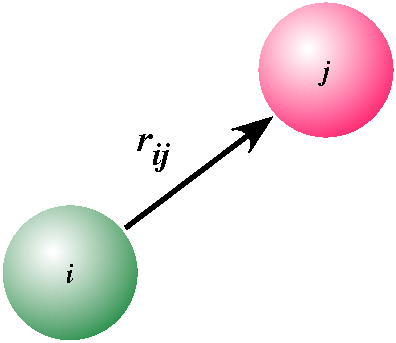
\includegraphics[width=2.5in]{bond.pdf}
\caption[Bond coordinates]{The coordinate describing a
a bond between atoms $i$ and $j$ is $|r_{ij}|$, the length of the
$\vec{r}_{ij}$ vector. } 
\label{fig:bond}
\end{figure}

OpenMD can also simulate some less common types of bond potentials,
including {\tt Fixed} bonds (which are constrained to be at a
specified bond length),
\begin{equation}
V_{\text{bond}}(b) = 0.
\end{equation}
{\tt Cubic} bonds include terms to model anharmonicity,
\begin{equation}
V_{\text{bond}}(b) =  K_3 (b -  b_{ij}^0)^3 + K_2 (b - b_{ij}^0)^2 + K_1 (b -  b_{ij}^0) + K_0,
\end{equation}
and {\tt Quartic} bonds, include another term in the Taylor
expansion around $b_{ij}^0$,
\begin{equation}
V_{\text{bond}}(b) = K_4 (b -  b_{ij}^0)^4 +  K_3 (b -  b_{ij}^0)^3 +
K_2 (b - b_{ij}^0)^2 + K_1 (b -  b_{ij}^0) + K_0,
\end{equation}
can also be simulated.  Note that the factor of $1/2$ that is included
in the {\tt Harmonic} bond type force constant is {\it not} present in
either the {\tt Cubic} or {\tt Quartic} bond types.

{\tt Polynomial} bonds which can have any number of terms,
\begin{equation}
V_{\text{bond}}(b) = \sum_n K_n (b -  b_{ij}^0)^n.
\end{equation}
can also be specified by giving a sequence of integer ($n$) and force
constant ($K_n$) pairs.

The order of terms in the BondTypes block is:
\begin{itemize}
\item {\tt AtomType} 1
\item {\tt AtomType} 2
\item {\tt BondType} (one of {\tt Harmonic}, {\tt Morse}, {\tt Fixed}, {\tt
        Cubic}, {\tt Quartic}, or {\tt Polynomial})
\item $b_{ij}^0$, the equilibrium bond length in \AA
\item any other parameters required by the {\tt BondType}
\end{itemize}

\begin{code}[caption={[An example of a BondTypes block.] A
simple example of a BondTypes block.  Distances ($b_0$)
are given in \AA\ and force constants are given in
units so that when multiplied by the correct power of distance they
return energies in kcal/mol.  For example $k$ for a Harmonic bond is
in units of kcal/mol/\AA$^2$.},
label={sch:BondTypes}]
begin BondTypes
//Atom1 Atom2   Harmonic        b0        k (kcal/mol/A^2)
CH2     CH2     Harmonic        1.526     260
//Atom1 Atom2   Morse           b0        D       beta (A^-1)
CN      NC      Morse           1.157437  212.95  2.5802
//Atom1 Atom2   Fixed           b0
CT      HC      Fixed           1.09
//Atom1 Atom2   Cubic           b0        K3      K2      K1      K0
//Atom1 Atom2   Quartic         b0        K4      K3      K2      K1      K0
//Atom1 Atom2   Polynomial      b0        n       Kn      [m      Km]
end BondTypes
\end{code}

There are advantages and disadvantages of all of the different types
of bonds, but specific simulation tasks may call for specific
behaviors.

\subsection{\label{section:ffBend}The {\tt BendTypes} block}
The equilibrium geometries and energy functions for bending motions in
a molecule are strongly dependent on the bonding environment of the
central atomic site.  For example, different types of hybridized
carbon centers require different bending angles and force constants to
describe the local geometry.

The bending potential energy functions used in most force fields are
often simple functions of the angle between two bonds,
\begin{equation}
\theta_{ijk} = \cos^{-1} \left(\frac{\vec{r}_{ji} \cdot
    \vec{r}_{jk}}{\left| \vec{r}_{ji} \right| \left| \vec{r}_{jk}
    \right|} \right)
\end{equation} 
Here atom $j$ is the central atom that is bonded to two partners $i$
and $k$.

\begin{figure}[h]
\centering
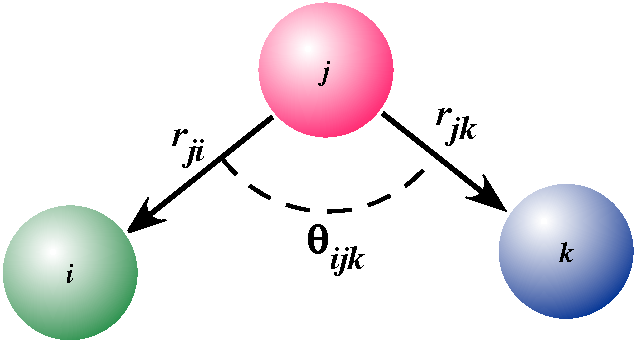
\includegraphics[width=3.5in]{bend.pdf}
\caption[Bend angle coordinates]{The coordinate describing a bend
  between atoms $i$, $j$, and $k$ is the angle $\theta_{ijk} =
  \cos^{-1} \left(\hat{r}_{ji} \cdot \hat{r}_{jk}\right)$ where $\hat{r}_{ji}$ is
  the unit vector between atoms $j$ and $i$. }
\label{fig:bend}
\end{figure}


All BendTypes must specify three AtomType names ($i$, $j$ and $k$)
that describe when that bend potential should be applied, as well as
an equilibrium bending angle, $\theta_{ijk}^0$, in units of
degrees. The most common forms for bending potentials are {\tt
  Harmonic} bends,
\begin{equation}
V_{\text{bend}}(\theta_{ijk}) = \frac{k_{ijk}}{2}( \theta_{ijk} - \theta_{ijk}^0
)^2, \label{eq:bendPot}
\end{equation}
where $k_{ijk}$ is the force constant which determines the strength of
the harmonic bend. {\tt UreyBradley} bends utilize an additional 1-3
bond-type interaction in addition to the harmonic bending potential:
\begin{equation}
V_{\text{bend}}(\vec{r}_i , \vec{r}_j, \vec{r}_k)
  =\frac{k_{ijk}}{2}( \theta_{ijk} - \theta_{ijk}^0)^2 
  + \frac{k_{ub}}{2}( r_{ik} - s_0 )^2. \label{eq:ubBend}
\end{equation}

A {\tt Cosine} bend is a variant on the harmonic bend which utilizes
the cosine of the angle instead of the angle itself,
\begin{equation}
V_{\text{bend}}(\theta_{ijk}) = \frac{k_{ijk}}{2}( \cos\theta_{ijk} -
\cos \theta_{ijk}^0 )^2. \label{eq:cosBend}
\end{equation}

OpenMD can also simulate some less common types of bend potentials,
including {\tt Cubic} bends, which include terms to model anharmonicity,
\begin{equation}
V_{\text{bend}}(\theta_{ijk}) =  K_3 (\theta_{ijk} -  \theta_{ijk}^0)^3 + K_2 (\theta_{ijk} -  \theta_{ijk}^0)^2 + K_1 (\theta_{ijk} -  \theta_{ijk}^0) + K_0,
\end{equation}
and {\tt Quartic} bends, which include another term in the Taylor
expansion around $\theta_{ijk}^0$,
\begin{equation}
  V_{\text{bend}}(\theta_{ijk}) = K_4 (\theta_{ijk} -  \theta_{ijk}^0)^4 +  K_3 (\theta_{ijk} -  \theta_{ijk}^0)^3 +
  K_2 (\theta_{ijk} -  \theta_{ijk}^0)^2 + K_1 (\theta_{ijk} -
  \theta_{ijk}^0) + K_0,
\end{equation}
can also be simulated.  Note that the factor of $1/2$ that is included
in the {\tt Harmonic} bend type force constant is {\it not} present in
either the {\tt Cubic} or {\tt Quartic} bend types.

{\tt Polynomial} bends which can have any number of terms,
\begin{equation}
V_{\text{bend}}(\theta_{ijk}) = \sum_n K_n (\theta_{ijk} -  \theta_{ijk}^0)^n.
\end{equation}
can also be specified by giving a sequence of integer ($n$) and force
constant ($K_n$) pairs.

The order of terms in the BendTypes block is:
\begin{itemize}
\item {\tt AtomType} 1
\item {\tt AtomType} 2 (this is the central atom)
\item {\tt AtomType} 3
\item {\tt BendType} (one of {\tt Harmonic}, {\tt UreyBradley}, {\tt
    Cosine}, {\tt Cubic}, {\tt Quartic}, or {\tt Polynomial})
\item $\theta_{ijk}^0$, the equilibrium bending angle in degrees.
\item any other parameters required by the {\tt BendType}
\end{itemize}

\begin{code}[caption={[An example of a BendTypes block.] A
simple example of a BendTypes block.  By convention, equilibrium angles
($\theta_0$) are given in degrees but force constants are given in
units so that when multiplied by the correct power of angle (in
radians) they return energies in kcal/mol.  For example $k$ for a 
Harmonic bend is in units of kcal/mol/radians$^2$.},
label={sch:BendTypes}]
begin BendTypes
//Atom1 Atom2   Atom3   Harmonic      theta0(deg) Ktheta(kcal/mol/radians^2)
CT      CT      CT      Harmonic      109.5        80.000000
CH2     CH      CH2     Harmonic      112.0       117.68
CH3     CH2     SH      Harmonic       96.0        67.220
//UreyBradley
//Atom1 Atom2   Atom3   UreyBradley   theta0      Ktheta  s0  Kub
//Cosine
//Atom1 Atom2   Atom3   Cosine        theta0      Ktheta(kcal/mol)
//Cubic
//Atom1 Atom2   Atom3   Cubic         theta0      K3      K2  K1   K0
//Quartic
//Atom1 Atom2   Atom3   Quartic       theta0      K4      K3  K2   K1   K0
//Polynomial
//Atom1 Atom2   Atom3   Polynomial    theta0      n       Kn  [m   Km]
end BendTypes
\end{code}

Note that the parameters for a particular bend type are the same for
any bending triplet of the same atomic types (in the same or reversed
order).  Changing the AtomType in the Atom2 position will change the
matched bend types in the force field.

\subsection{\label{section:ffTorsion}The {\tt TorsionTypes} block}
The torsion potential for rotation of groups around a central bond can
often be represented with various cosine functions.  For two
tetrahedral ($sp^3$) carbons connected by a single bond, the torsion
potential might be
\begin{equation*}
V_{\text{torsion}} = \frac{v}{2} \left[ 1 + \cos( 3 \phi ) \right]
\end{equation*}
where $v$ is the barrier for going from {\em staggered} $\rightarrow$
{\em eclipsed} conformations, while for $sp^2$ carbons connected by a
double bond, the potential might be
\begin{equation*}
V_{\text{torsion}} = \frac{w}{2} \left[ 1 - \cos( 2 \phi ) \right]
\end{equation*}
where $w$ is the barrier for going from  {\em cis} $\rightarrow$ {\em
  trans} conformations.

A general torsion potentials can be represented as a cosine series of
the form:
\begin{equation}
V_{\text{torsion}}(\phi_{ijkl}) = c_1[1 + \cos \phi_{ijkl}] 
	+ c_2[1 - \cos(2\phi_{ijkl})] 
 	+ c_3[1 + \cos(3\phi_{ijkl})],
\label{eq:origTorsionPot}
\end{equation}
where the angle $\phi_{ijkl}$ is defined 
\begin{equation}
\cos\phi_{ijkl} = (\hat{\mathbf{r}}_{ij} \times \hat{\mathbf{r}}_{jk}) \cdot
	(\hat{\mathbf{r}}_{jk} \times \hat{\mathbf{r}}_{kl}).
\label{eq:torsPhi}
\end{equation}
Here, $\hat{\mathbf{r}}_{\alpha\beta}$ are the set of unit bond
vectors between atoms $i$, $j$, $k$, and $l$.  Note that some force
fields define the zero of the $\phi_{ijkl}$ angle when atoms $i$ and
$l$ are in the {\em trans} configuration, while most define the zero
angle for when $i$ and $l$ are in the fully eclipsed orientation.  The
behavior of the torsion parser can be altered with the {\tt
  TorsionAngleConvention} keyword in the Options block.  The default
behavior is {\tt "180\_is\_trans"} while the opposite behavior can be
invoked by setting this keyword to {\tt "0\_is\_trans"}.

\begin{figure}[h]
\centering
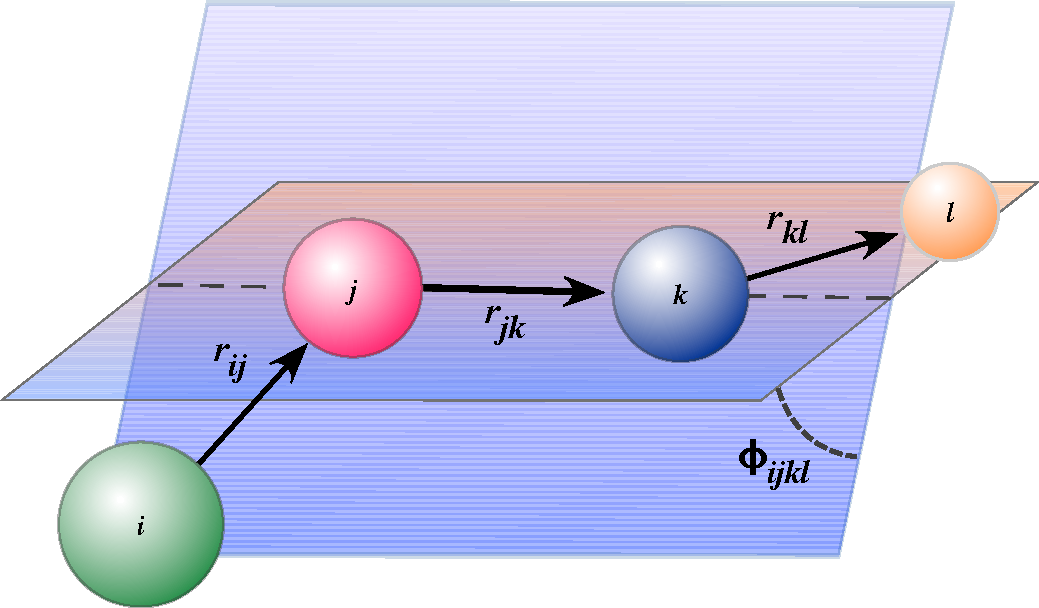
\includegraphics[width=4.5in]{torsion.pdf}
\caption[Torsion or dihedral angle coordinates]{The coordinate
  describing a torsion between atoms $i$, $j$, $k$, and $l$ is the
  dihedral angle $\phi_{ijkl}$ which measures the relative rotation of
  the two terminal atoms around the axis defined by the middle bond. }
\label{fig:torsion}
\end{figure}

For computational efficiency, OpenMD recasts torsion potential in the
method of CHARMM,\cite{Brooks83} in which the angle series is
converted to a power series of the form:
\begin{equation}
  V_{\text{torsion}}(\phi_{ijkl}) =  
  k_3 \cos^3 \phi_{ijkl} + k_2 \cos^2 \phi_{ijkl} + k_1 \cos \phi_{ijkl} + k_0,
\label{eq:torsionPot}
\end{equation}
where:
\begin{align*}
k_0 &= c_1 + 2 c_2 + c_3, \\
k_1 &= c_1 - 3c_3, \\
k_2 &= - 2 c_2, \\
k_3 &= 4 c_3.
\end{align*}
By recasting the potential as a power series, repeated trigonometric
evaluations are avoided during the calculation of the potential
energy.

Using this framework, OpenMD implements a variety of different
potential energy functions for torsions:
\begin{itemize}
\item {\tt Cubic}:
\begin{equation*}
  V_{\text{torsion}}(\phi) =  
  k_3 \cos^3 \phi + k_2 \cos^2 \phi + k_1 \cos \phi + k_0
\end{equation*}
\item {\tt Quartic}:
\begin{equation*}
  V_{\text{torsion}}(\phi) =  k_4 \cos^4 \phi + 
  k_3 \cos^3 \phi + k_2 \cos^2 \phi + k_1 \cos \phi + k_0
\end{equation*}
\item {\tt Polynomial}:
\begin{equation*}
V_{\text{torsion}}(\phi) =  \sum_n k_n \cos^n \phi 
\end{equation*}
\item {\tt Charmm}:
\begin{equation*}
V_{\text{torsion}}(\phi) = \sum_n K_n \left( 1 + cos(n
  \phi - \delta_n) \right)
\end{equation*}
\item {\tt Opls}:
\begin{equation*}
  V_{\text{torsion}}(\phi) =  \frac{1}{2} \left(v_1 (1 + \cos \phi)
    + v_2 (1 - \cos 2 \phi) +  v_3 (1 + \cos 3 \phi)  \right)
\end{equation*}
\item {\tt Trappe}:\cite{Siepmann1998}
\begin{equation*}
  V_{\text{torsion}}(\phi) =  c_0 + c_1 (1 + \cos \phi) + c_2 (1 - \cos 2 \phi)  +
  c_3 (1 + \cos 3 \phi)
\end{equation*}
\item {\tt Harmonic}:
\begin{equation*}
V_{\text{torsion}}(\phi) =  \frac{d_0}{2} \left(\phi - \phi^0\right)^2
\end{equation*}
\end{itemize}

Most torsion types don't require specific angle information in the
parameters since they are typically expressed in cosine polynomials.
{\tt Charmm} and {\tt Harmonic} torsions are a bit different.  {\tt
  Charmm} torsion types require a set of phase angles, $\delta_n$ that
are expressed in degrees, and associated periodicity numbers, $n$.
{\tt Harmonic} torsions have an equilibrium torsion angle, $\phi_0$
that is measured in degrees, while $d_0$ has units of
kcal/mol/degrees$^2$.  All other torsion parameters are measured in
units of kcal/mol.

\begin{code}[caption={[An example of a TorsionTypes block.] A
simple example of a TorsionTypes block.  Energy constants are given in
kcal / mol, and when required by the form, $\delta$ angles are given
in degrees.},
label={sch:TorsionTypes}]
begin TorsionTypes
//Cubic
//Atom1 Atom2   Atom3   Atom4   Cubic   k3       k2        k1      k0  
CH2     CH2     CH2     CH2     Cubic   5.9602   -0.2568   -3.802  2.1586
CH2     CH      CH      CH2     Cubic   3.3254   -0.4215   -1.686  1.1661
//Trappe
//Atom1 Atom2   Atom3   Atom4   Trappe  c0       c1        c2      c3
CH3     CH2     CH2     SH      Trappe  0.10507  -0.10342  0.03668 0.60874     
//Charmm
//Atom1 Atom2   Atom3   Atom4   Charmm  Kchi     n    delta  [Kchi n delta]
CT      CT      CT      C       Charmm  0.156    3    0.00
OH      CT      CT      OH      Charmm  0.144    3    0.00    1.175 2  0
HC      CT      CM      CM      Charmm  1.150    1    0.00    0.38  3 180
//Quartic
//Atom1 Atom2   Atom3   Atom4   Quartic          k4    k3    k2    k1    k0
//Polynomial
//Atom1 Atom2   Atom3   Atom4   Polynomial  n Kn [m  Km] 
S       CH2     CH2     C   Polynomial 0 2.218 1 2.905 2 -3.136 3 -0.7313 4 6.272 5 -7.528
end TorsionTypes
\end{code}

Note that the parameters for a particular torsion type are the same
for any torsional quartet of the same atomic types (in the same or
reversed order).

\subsection{\label{section:ffInversion}The {\tt InversionTypes} block}

Inversion potentials are often added to force fields to enforce
planarity around $sp^2$-hybridized carbons or to correct vibrational
frequencies for umbrella-like vibrational modes for central atoms
bonded to exactly three satellite groups.

In OpenMD's version of an inversion, the central atom is entered {\it
  first} in each line in the {\tt InversionTypes} block. Note that
this is quite different than how other codes treat Improper torsional
potentials to mimic inversion behavior.  In some other widely-used
simulation packages, the central atom is treated as atom 3 in a
standard torsion form:
\begin{itemize}
  \item OpenMD:  I - (J - K - L)  (e.g. I is $sp^2$ hybridized carbon)
  \item AMBER:   I - J - K - L   (e.g. K is $sp^2$ hybridized carbon)
\end{itemize}

The inversion angle itself is defined as:
\begin{equation}
\cos\omega_{i-jkl} = \left(\hat{\mathbf{r}}_{il} \times
  \hat{\mathbf{r}}_{ij}\right)\cdot\left( \hat{\mathbf{r}}_{il} \times
  \hat{\mathbf{r}}_{ik}\right)
\end{equation}
Here, $\hat{\mathbf{r}}_{\alpha\beta}$ are the set of unit bond
vectors between the central atoms $i$, and the satellite atoms $j$,
$k$, and $l$.  Note that other definitions of inversion angles are
possible, so users are encouraged to be particularly careful when
converting other force field files for use with OpenMD.

There are many common ways to create planarity or umbrella behavior in
a potential energy function, and OpenMD implements a number of the
more common functions:
\begin{itemize}
\item {\tt ImproperCosine}:
\begin{equation*}
V_{\text{torsion}}(\omega) = \sum_n \frac{K_n}{2} \left( 1 + cos(n
  \omega - \delta_n) \right),
\end{equation*}
\item {\tt AmberImproper}:
\begin{equation*}
  V_{\text{torsion}}(\omega) =  \frac{v}{2} (1 - \cos\left(2 \left(\omega - \omega_0\right)\right),
\end{equation*}
\item {\tt Harmonic}:
\begin{equation*}
V_{\text{torsion}}(\omega) =  \frac{d}{2} \left(\omega - \omega_0\right)^2.
\end{equation*}
\end{itemize}
\begin{code}[caption={[An example of an InversionTypes block.] A
simple example of a InversionTypes block.  Angles ($\delta_n$ and
$\omega_0$) angles are given in degrees, while energy parameters ($v,
K_n$) are given in kcal / mol.   The Harmonic Inversion type has a
force constant that must be given in kcal/mol/degrees$^2$.},
label={sch:InversionTypes}]
begin InversionTypes
//Harmonic
//Atom1 Atom2   Atom3   Atom4   Harmonic  d(kcal/mol/deg^2)  omega0
RCHar3  X       X       X       Harmonic  1.21876e-2         180.0
//AmberImproper
//Atom1 Atom2   Atom3   Atom4   AmberImproper   v(kcal/mol)
C       CT      N       O       AmberImproper   10.500000
CA      CA      CA      CT      AmberImproper   1.100000 
//ImproperCosine
//Atom1 Atom2   Atom3   Atom4   ImproperCosine  Kn  n  delta_n  [Kn n delta_n]
end InversionTypes
\end{code}

\section{\label{section::ffLongRange}Long Range Interactions}

Calculating the long-range (non-bonded) potential involves a sum over
all pairs of atoms (except for those atoms which are involved in a
bond, bend, or torsion with each other).  Many of these interactions
can be inferred from the AtomTypes,

\subsection{\label{section:ffNBinteraction}The {\tt NonBondedInteractions}
  block}

The user might want like to specify explicit or special interactions
that override the default non-bonded interactions that are inferred
from the AtomTypes.  To do this, OpenMD implements a
NonBondedInteractions block to allow the user to specify the following
(pair-wise) non-bonded interactions:

\begin{itemize}
\item {\tt LennardJones}:
\begin{equation*}
V_{\text{NB}}(r) = 4 \epsilon_{ij} \left(
  \left(\frac{\sigma_{ij}}{r} \right)^{12} -
  \left(\frac{\sigma_{ij}}{r} \right)^{6} \right),
\end{equation*}
\item {\tt ShiftedMorse}:
\begin{equation*}
 V_{\text{NB}}(r) = D_{ij} \left( e^{-2 \beta_{ij} (r -
     r_0)} - 2 e^{- \beta_{ij} (r -
     r_0)} \right),
\end{equation*}
\item {\tt RepulsiveMorse}:
\begin{equation*}
 V_{\text{NB}}(r) = D_{ij} \left( e^{-2 \beta_{ij} (r -
     r_0)} \right),
\end{equation*}
\item {\tt RepulsivePower}:
\begin{equation*}
  V_{\text{NB}}(r) = \epsilon_{ij}
  \left(\frac{\sigma_{ij}}{r} \right)^{n_{ij}}.
\end{equation*}
\item {\tt Mie}:
\begin{equation*}
  V_{\text{NB}}(r) =  \left(\frac{n}{n-m}\right)
  \left(\frac{n}{m}\right)^{m/(n-m)} \epsilon_{ij} \left[
  \left(\frac{\sigma_{ij}}{r} \right)^{n} -
  \left(\frac{\sigma_{ij}}{r} \right)^{m} \right].
\end{equation*}
\item {\tt Buckingham Traditional}:
\begin{equation*}
  V_{\text{NB}}(r) =  A \exp( -B r) - \frac{C}{r^6}.
\end{equation*}
\item {\tt Buckingham Modified}:
\begin{equation*}
  V_{\text{NB}}(r) = A \exp( -B r) - \frac{C}{r^6} + 4 \epsilon \left( \left( \frac{\sigma}{r} \right)^{30} - \left( \frac{\sigma}{r} \right)^6 \right).
\end{equation*}
\item {\tt EAMZhou} (pair potential only):
\begin{equation*}
  V_{\text{NB}}(r) = \frac{ A \exp\left[-\alpha (r/r_e -1)\right]}{1+(r/r_e - \kappa)^{20}} -  \frac{ B \exp\left[-\beta (r/r_e -1)\right]}{1+(r/r_e - \lambda)^{20}}
\end{equation*}
\item {\tt InversePowerSeries}:
\begin{equation*}
  V_{\text{NB}}(r) = \sum_{n} \frac{ c_n }{ r_{ij}^n}.
\end{equation*}

\end{itemize}

\begin{code}[caption={[An example of a NonBondedInteractions block.] A
simple example of a NonBondedInteractions block. Distances ($\sigma,
r_0$) are given in \AA, while energies ($\epsilon, D0$) are in
kcal/mol.  The Morse potentials have an additional parameter $\beta_0$
which is in units of \AA$^{-1}$.},
label={sch:NonBondedInteractionTypes}]
begin NonBondedInteractions

//Lennard-Jones
//Atom1 Atom2   LennardJones    sigma  epsilon
Au      CH3     LennardJones    3.54   0.2146
Au      CH2     LennardJones    3.54   0.1749 
Au      CH      LennardJones    3.54   0.1749 
Au      S       LennardJones    2.40   8.465

//Shifted Morse
//Atom1 Atom2   ShiftedMorse    r0     D0       beta0
Au      O_SPCE  ShiftedMorse    3.70   0.0424   0.769

//Repulsive Morse
//Atom1 Atom2   RepulsiveMorse  r0     D0       beta0
Au      H_SPCE  RepulsiveMorse  -1.00  0.00850  0.769

//Repulsive Power
//Atom1 Atom2   RepulsivePower   sigma    epsilon    n
Au      ON      RepulsivePower   3.47005  0.186208   11
Au      NO      RepulsivePower   3.53955  0.168629   11

//Mie potential
//Atom1 Atom2   Mie              sigma   epsilon  n  m
Ar      Au      Mie              3.41    0.234   12  3

//Buckingham Traditional      A (kcal/mol)  B(A-1)   C(kcal/mol/A^6)
Si O Buckingham Traditional   415176.39808  4.87318  3079.46096

//Buckingham Modified    A (kcal/mol)  B(A-1)  C(kcal/mol/A^6) sigma    epsilon
Si O Buckingham Modified 415179.721807 4.87318 3079.48551137   1.779239 0.02423780013

//Types       re        alpha   beta    A (eV)  B (eV)  kappa   lambda
Al Ni EAMZhou 2.71579   8.00443 4.75970 0.44254 0.68349 0.63279 0.81777
// note that EAM force fields usually have the MetallicEnergyUnitScaling 
// option set to 23.0605423 for energy units of A and B.

end NonBondedInteractions
\end{code}

\section{\label{section:electrostatics}Electrostatics}

Because nearly all force fields involve electrostatic interactions in
one form or another, OpenMD implements a number of different
electrostatic summation methods.  These methods are extended from the
damped and cutoff-neutralized Coulombic sum originally proposed by
Wolf, {\it et al.}\cite{Wolf99} One of these, the damped shifted force
method, shows a remarkable ability to reproduce the energetic and
dynamic characteristics exhibited by simulations employing lattice
summation techniques.  The basic idea is to construct well-behaved
real-space summation methods using two tricks:
\begin{enumerate}
\item shifting through the use of image charges, and 
\item damping the electrostatic interaction.
\end{enumerate} 
Starting with the original observation that the effective range of the
electrostatic interaction in condensed phases is considerably less
than $r^{-1}$, either the cutoff sphere neutralization or the
distance-dependent damping technique could be used as a foundation for
a new pairwise summation method.  Wolf \textit{et al.} made the
observation that charge neutralization within the cutoff sphere plays
a significant role in energy convergence; therefore we will begin our
analysis with the various shifted forms that maintain this charge
neutralization.  We can evaluate the methods of Wolf
\textit{et al.}  and Zahn \textit{et al.} by considering the standard
shifted potential,
\begin{equation}
V_\textrm{SP}(r) =      \begin{cases}
v(r)-v_\textrm{c} &\quad r\leqslant R_\textrm{c} \\ 0 &\quad r >
R_\textrm{c}  
\end{cases},
\label{eq:shiftingPotForm}
\end{equation}
and shifted force,
\begin{equation}
V_\textrm{SF}(r) =      \begin{cases}
v(r)-v_\textrm{c}-\left(\frac{d v(r)}{d r}\right)_{r=R_\textrm{c}}(r-R_\textrm{c
})
&\quad r\leqslant R_\textrm{c} \\ 0 &\quad r > R_\textrm{c} 
                                                \end{cases},
\label{eq:shiftingForm}
\end{equation}
functions where $v(r)$ is the unshifted form of the potential, and
$v_c$ is $v(R_\textrm{c})$.  The Shifted Force (SF) form ensures
that both the potential and the forces goes to zero at the cutoff
radius, while the Shifted Potential (SP) form only ensures the
potential is smooth at the cutoff radius
($R_\textrm{c}$).\cite{Allen87}

The forces associated with the shifted potential are simply the forces
of the unshifted potential itself (when inside the cutoff sphere),
\begin{equation}
F_{\textrm{SP}} = -\left( \frac{d v(r)}{dr} \right),
\end{equation}
and are zero outside.  Inside the cutoff sphere, the forces associated
with the shifted force form can be written,
\begin{equation}
F_{\textrm{SF}} = -\left( \frac{d v(r)}{dr} \right) + \left(\frac{d
v(r)}{dr} \right)_{r=R_\textrm{c}}.
\end{equation}
 
If the potential, $v(r)$, is taken to be the normal Coulomb potential,
\begin{equation}
v(r) = \frac{q_i q_j}{r},
\label{eq:Coulomb}
\end{equation}
then the Shifted Potential (SP) forms will give Wolf {\it et
al.}'s undamped prescription:
\begin{equation}
V_\textrm{SP}(r) =
q_iq_j\left(\frac{1}{r}-\frac{1}{R_\textrm{c}}\right) \quad
r\leqslant R_\textrm{c},
\label{eq:SPPot}
\end{equation}
with associated forces,
\begin{equation}
F_\textrm{SP}(r) = q_iq_j\left(\frac{1}{r^2}\right) \quad r\leqslant R_\textrm{c
}.
\label{eq:SPForces}
\end{equation}
These forces are identical to the forces of the standard Coulomb
interaction, and cutting these off at $R_c$ was addressed by Wolf
\textit{et al.} as undesirable.  They pointed out that the effect of
the image charges is neglected in the forces when this form is
used,\cite{Wolf99} thereby eliminating any benefit from the method in
molecular dynamics.  Additionally, there is a discontinuity in the
forces at the cutoff radius which results in energy drift during MD
simulations.

The shifted force (SF) form using the normal Coulomb potential
will give,
\begin{equation}
V_\textrm{SF}(r) = q_iq_j\left[\frac{1}{r}-\frac{1}{R_\textrm{c}}+\left(\frac{1}
{R_\textrm{c}^2}\right)(r-R_\textrm{c})\right] \quad r\leqslant R_\textrm{c}.
\label{eq:SFPot}
\end{equation}
with associated forces,
\begin{equation}
F_\textrm{SF}(r) =  q_iq_j\left(\frac{1}{r^2}-\frac{1}{R_\textrm{c}^2}\right) \quad r\leqslant R_\textrm{c}.
\label{eq:SFForces}
\end{equation}
This formulation has the benefits that there are no discontinuities at
the cutoff radius, while the neutralizing image charges are present in
both the energy and force expressions.  It would be simple to add the
self-neutralizing term back when computing the total energy of the
system, thereby maintaining the agreement with the Madelung energies.
A side effect of this treatment is the alteration in the shape of the
potential that comes from the derivative term.  Thus, a degree of
clarity about agreement with the empirical potential is lost in order
to gain functionality in dynamics simulations.

Wolf \textit{et al.} originally discussed the energetics of the
shifted Coulomb potential (Eq. \ref{eq:SPPot}) and found that it was
insufficient for accurate determination of the energy with reasonable
cutoff distances.  The calculated Madelung energies fluctuated around
the expected value as the cutoff radius was increased, but the
oscillations converged toward the correct value.\cite{Wolf99} A
damping function was incorporated to accelerate the convergence; and
though alternative forms for the damping function could be
used,\cite{Jones56,Heyes81} the complimentary error function was
chosen to mirror the effective screening used in the Ewald summation.
Incorporating this error function damping into the simple Coulomb
potential,
\begin{equation}
v(r) = \frac{\mathrm{erfc}\left(\alpha r\right)}{r},
\label{eq:dampCoulomb}
\end{equation}
the shifted potential (eq. (\ref{eq:SPPot})) becomes
\begin{equation}
V_{\textrm{DSP}}(r) = q_iq_j\left(\frac{\textrm{erfc}\left(\alpha r\right)}{r}-\frac{\textrm{erfc}\left(\alpha R_\textrm{c}\right)}{R_\textrm{c}}\right) \quad r
\leqslant R_\textrm{c},
\label{eq:DSPPot}
\end{equation}
with associated forces,
\begin{equation}
F_{\textrm{DSP}}(r) = q_iq_j\left(\frac{\textrm{erfc}\left(\alpha r\right)}{r^2}
+\frac{2\alpha}{\pi^{1/2}}\frac{\exp{\left(-\alpha^2r^2\right)}}{r}\right) \quad
 r\leqslant R_\textrm{c}.
\label{eq:DSPForces}
\end{equation}
Again, this damped shifted potential suffers from a
force-discontinuity at the cutoff radius, and the image charges play
no role in the forces.  To remedy these concerns, one may derive a
SF variant by including the derivative term in
eq. (\ref{eq:shiftingForm}),
\begin{equation}
\begin{split}
V_\mathrm{DSF}(r) = q_iq_j\Biggr{[} & \frac{\mathrm{erfc}\left(\alpha r \right)}{r} -\frac{\mathrm{erfc}\left(\alpha R_\mathrm{c} \right) }{R_\mathrm{c}} \\
 & \left. +\left(\frac{\mathrm{erfc}\left(\alpha
R_\mathrm{c}\right)}{R_\mathrm{c}^2}+\frac{2\alpha}{\pi^{1/2}}\frac{\exp\left(-\alpha^2R_\mathrm{c}^2\right)}{R_\mathrm{c}}\right)\left(r-R_\mathrm{c}\right)
\right] \quad r\leqslant R_\textrm{c} 
\label{eq:DSFPot}
\end{split}
\end{equation}
The derivative of the above potential will lead to the following forces,
\begin{equation}
\begin{split}
F_\mathrm{DSF}(r) =
q_iq_j\Biggr{[}&\left(\frac{\textrm{erfc}\left(\alpha r\right)}{r^2}+\frac{2\alpha}{\pi^{1/2}}\frac{\exp{\left(-\alpha^2r^2\right)}}{r}\right) \\ &\left.-\left(\frac{\textrm{erfc}\left(\alpha R_{\textrm{c}}\right)}{R_{\textrm{c}}^2}+\frac{2\alpha}{\pi^{1/2}}\frac{\exp{\left(-\alpha^2R_{\textrm{c}}^2
\right)}}{R_{\textrm{c}}}\right)\right] \quad r\leqslant R_\textrm{c}.
\label{eq:DSFForces}
\end{split}
\end{equation}
If the damping parameter $(\alpha)$ is set to zero, the undamped case,
eqs. (\ref{eq:SPPot} through \ref{eq:SFForces}) are correctly
recovered from eqs. (\ref{eq:DSPPot} through \ref{eq:DSFForces}).

It has been shown that the Damped Shifted Force method obtains nearly
identical behavior to the smooth particle mesh Ewald (SPME)
method on a number of commonly simulated systems.\cite{Fennell06}  For
this reason, the default electrostatic summation method utilized by
OpenMD is the DSF (Eq. \ref{eq:DSFPot}) with a damping parameter
($\alpha$) that is set algorithmically from the cutoff radius.

For interactions involving point dipoles and quadrupoles, the shifted potential and shifted force methods have been generalized for multipolar interactions.\cite{Lamichhane:2014yg,Lamichhane:2014eu,Lamichhane:2016uq} 
Setting  {\tt cutoffMethod = TAYLOR\_SHIFTED;} provides an additional option, but the default, {\tt cutoffMethod = SHIFTED\_FORCE;} also known as the \textbf{Gradient Shifted} approximation, should provide good behavior for most multipoles in common molecular dynamics simulations.  Readers interested in the differences between these two shifted methods should consult Refs. \citenum{Lamichhane:2014eu} and \citenum{Lamichhane:2016uq}.

\section{\label{section:cutoffGroups}Switching Functions}

Calculating the the long-range interactions for $N$ atoms involves
$N(N-1)/2$ evaluations of atomic distances if it is done in a brute
force manner.  To reduce the number of distance evaluations between
pairs of atoms, OpenMD allows the use of hard or switched
cutoffs with Verlet neighbor lists.\cite{Allen87} Neutral groups which
contain charges can exhibit pathological forces unless the cutoff is
applied to the neutral groups evenly instead of to the individual
atoms.\cite{leach01:mm} OpenMD allows users to specify cutoff
groups which may contain an arbitrary number of atoms in the molecule.
Atoms in a cutoff group are treated as a single unit for the
evaluation of the switching function:
\begin{equation}
V_{\mathrm{long-range}} = \sum_{a} \sum_{b>a} s(r_{ab}) \sum_{i \in a} \sum_{j \in b} V_{ij}(r_{ij}),
\end{equation}
where $r_{ab}$ is the distance between the centers of mass of the two
cutoff groups ($a$ and $b$).

The sums over $a$ and $b$ are over the cutoff groups that are present
in the simulation.  Atoms which are not explicitly defined as members
of a {\tt cutoffGroup} are treated as a group consisting of only one
atom.  The switching function, $s(r)$ is the standard cubic switching
function,
\begin{equation}
S(r) = 
	\begin{cases}
	1 & \text{if $r \le r_{\text{sw}}$},\\
	\frac{(r_{\text{cut}} + 2r - 3r_{\text{sw}})(r_{\text{cut}} - r)^2}
	{(r_{\text{cut}} - r_{\text{sw}})^3} 
	& \text{if $r_{\text{sw}} < r \le r_{\text{cut}}$}, \\
	0 & \text{if $r > r_{\text{cut}}$.}
	\end{cases}
\label{eq:dipoleSwitching}
\end{equation}
Here, $r_{\text{sw}}$ is the {\tt switchingRadius}, or the distance
beyond which interactions are reduced, and $r_{\text{cut}}$ is the
{\tt cutoffRadius}, or the distance at which interactions are
truncated.  

Users of OpenMD do not need to specify the {\tt cutoffRadius} or
{\tt switchingRadius}.   
If the {\tt cutoffRadius} was not explicitly set, OpenMD will attempt
to guess an appropriate choice.  If the system contains electrostatic
atoms, the default cutoff radius is 12 \AA.  In systems without
electrostatic (charge or multipolar) atoms, the atom types present in the simulation will be
polled for suggested cutoff values (e.g. $2.5 max(\left\{ \sigma
  \right\})$ for Lennard-Jones atoms.   The largest suggested value
that was found will be used.

By default, OpenMD uses shifted force potentials to force the
potential energy and forces to smoothly approach zero at the cutoff
radius.  If the user would like to use another cutoff method
they may do so by setting the {\tt cutoffMethod} parameter to:
\begin{itemize}
\item {\tt HARD}
\item {\tt SWITCHED}
\item {\tt SHIFTED\_FORCE} (default):
\item {\tt TAYLOR\_SHIFTED}
\item {\tt SHIFTED\_POTENTIAL}
\end{itemize}

The {\tt switchingRadius} is set to a default value of 95\% of the
{\tt cutoffRadius}.  In the special case of a simulation containing
{\it only} Lennard-Jones atoms, the default switching radius takes the
same value as the cutoff radius, and OpenMD will use a shifted
potential to remove discontinuities in the potential at the cutoff.
Both radii may be specified in the meta-data file.

\section{\label{section:pbc}Periodic Boundary Conditions} 

\newcommand{\roundme}{\operatorname{round}}

\textit{Periodic boundary conditions} are widely used to simulate bulk
properties with a relatively small number of particles. In this method
the simulation box is replicated throughout space to form an infinite
lattice.  During the simulation, when a particle moves in the primary
cell, its image in other cells move in exactly the same direction with
exactly the same orientation. Thus, as a particle leaves the primary
cell, one of its images will enter through the opposite face. If the
simulation box is large enough to avoid ``feeling'' the symmetries of
the periodic lattice, surface effects can be ignored. The available
periodic cells in OpenMD are cubic, orthorhombic and
parallelepiped.  OpenMD use a $3 \times 3$ matrix, $\mathsf{H}$,
to describe the shape and size of the simulation box. $\mathsf{H}$ is
defined:
\begin{equation}
\mathsf{H} = ( \mathbf{h}_x, \mathbf{h}_y, \mathbf{h}_z ),
\end{equation}
where $\mathbf{h}_{\alpha}$ is the column vector of the $\alpha$ axis of the
box.  During the course of the simulation both the size and shape of
the box can be changed to allow volume fluctuations when constraining
the pressure.

A real space vector, $\mathbf{r}$ can be transformed in to a box space
vector, $\mathbf{s}$, and back through the following transformations:
\begin{align}
\mathbf{s} &= \mathsf{H}^{-1} \mathbf{r}, \\
\mathbf{r} &= \mathsf{H} \mathbf{s}.
\end{align}
The vector $\mathbf{s}$ is now a vector expressed as the number of box
lengths in the $\mathbf{h}_x$, $\mathbf{h}_y$, and $\mathbf{h}_z$
directions. To find the minimum image of a vector $\mathbf{r}$,
OpenMD first converts it to its corresponding vector in box space, and
then casts each element to lie in the range $[-0.5,0.5]$:
\begin{equation}
s_{i}^{\prime}=s_{i}-\roundme(s_{i}),
\end{equation}
where $s_i$ is the $i$th element of $\mathbf{s}$, and
$\roundme(s_i)$ is given by
\begin{equation}
\roundme(x) =
	\begin{cases}
	\lfloor x+0.5 \rfloor & \text{if $x \ge 0$,} \\
	\lceil x-0.5 \rceil & \text{if $x < 0$.}
	\end{cases}
\end{equation}
Here $\lfloor x \rfloor$ is the floor operator, and gives the largest
integer value that is not greater than $x$, and $\lceil x \rceil$ is
the ceiling operator, and gives the smallest integer that is not less
than $x$. 

Finally, the minimum image coordinates $\mathbf{r}^{\prime}$ are
obtained by transforming back to real space,
\begin{equation}
\mathbf{r}^{\prime} = \mathsf{H} \mathbf{s}^{\prime}.%
\end{equation}
In this way, particles are allowed to diffuse freely in $\mathbf{r}$,
but their minimum images, or $\mathbf{r}^{\prime}$, are used to compute
the inter-atomic forces.

\chapter{\label{section:mechanics}Mechanics}

\section{\label{section:integrate}Integrating the Equations of Motion: the
DLM method}

The default method for integrating the equations of motion in 
OpenMD is a velocity-Verlet version of the symplectic splitting method
proposed by Dullweber, Leimkuhler and McLachlan
(DLM).\cite{Dullweber1997} When there are no directional atoms or
rigid bodies present in the simulation, this integrator becomes the
standard velocity-Verlet integrator which is known to sample the
microcanonical (NVE) ensemble.\cite{Frenkel1996}

Previous integration methods for orientational motion have problems
that are avoided in the DLM method.  Direct propagation of the Euler
angles has a known $1/\sin\theta$ divergence in the equations of
motion for $\phi$ and $\psi$,\cite{Allen87} leading to numerical
instabilities any time one of the directional atoms or rigid bodies
has an orientation near $\theta=0$ or $\theta=\pi$.  Quaternion-based
integration methods work well for propagating orientational motion;
however, energy conservation concerns arise when using the
microcanonical (NVE) ensemble.  An earlier implementation of
OpenMD utilized quaternions for propagation of rotational motion;
however, a detailed investigation showed that they resulted in a
steady drift in the total energy, something that has been observed by
Laird {\it et al.}\cite{Laird97}

The key difference in the integration method proposed by Dullweber
\emph{et al.} is that the entire $3 \times 3$ rotation matrix is
propagated from one time step to the next. In the past, this would not
have been feasible, since the rotation matrix for a single body has
nine elements compared with the more memory-efficient methods (using
three Euler angles or 4 quaternions).  Computer memory has become much
less costly in recent years, and this can be translated into
substantial benefits in energy conservation.

The basic equations of motion being integrated are derived from the
Hamiltonian for conservative systems containing rigid bodies,
\begin{equation}
H = \sum_{i} \left( \frac{1}{2} m_i \mathbf{v}_i^T \cdot \mathbf{v}_i +
\frac{1}{2} \mathbf{j}_i^T \cdot \overleftrightarrow{\mathsf{I}}_i^{-1} \cdot
\mathbf{j}_i \right) +
V\left(\left\{\mathbf{r}\right\}, \left\{\mathsf{A}\right\}\right),
\end{equation}
where $\mathbf{r}_i$ and $\mathbf{v}_i$ are the cartesian position vector
and velocity of the center of mass of particle $i$, and $\mathbf{j}_i$,
$\overleftrightarrow{\mathsf{I}}_i$ are the body-fixed angular
momentum and moment of inertia tensor respectively, and the
superscript $T$ denotes the transpose of the vector.  $\mathsf{A}_i$
is the $3 \times 3$ rotation matrix describing the instantaneous
orientation of the particle.  $V$ is the potential energy function
which may depend on both the positions $\left\{\mathbf{r}\right\}$ and
orientations $\left\{\mathsf{A}\right\}$ of all particles.  The
equations of motion for the particle centers of mass are derived from
Hamilton's equations and are quite simple,
\begin{eqnarray}
\dot{\mathbf{r}} & = & \mathbf{v}, \\
\dot{\mathbf{v}} & = & \frac{\mathbf{f}}{m},
\end{eqnarray}
where $\mathbf{f}$ is the instantaneous force on the center of mass
of the particle,
\begin{equation}
\mathbf{f} = - \frac{\partial}{\partial
\mathbf{r}} V(\left\{\mathbf{r}(t)\right\}, \left\{\mathsf{A}(t)\right\}).
\end{equation}

The equations of motion for the orientational degrees of freedom are
\begin{eqnarray}
\dot{\mathsf{A}} & = & \mathsf{A} \cdot
\mbox{ skew}\left(\overleftrightarrow{\mathsf{I}}^{-1} \cdot \mathbf{j}\right),\\
\dot{\mathbf{j}} & = & \mathbf{j} \times \left( \overleftrightarrow{\mathsf{I}}^{-1}
\cdot \mathbf{j} \right) - \mbox{ rot}\left(\mathsf{A}^{T} \cdot \frac{\partial
V}{\partial \mathsf{A}} \right).
\end{eqnarray}
In these equations of motion, the $\mbox{skew}$ matrix of a vector
$\mathbf{v} = \left( v_1, v_2, v_3 \right)$ is defined:
\begin{equation}
\mbox{skew}\left( \mathbf{v} \right) := \left( 
\begin{array}{ccc}
0 & v_3 & - v_2 \\
-v_3 & 0 & v_1 \\
v_2 & -v_1 & 0 
\end{array}
\right).
\end{equation}
The $\mbox{rot}$ notation refers to the mapping of the $3 \times 3$
rotation matrix to a vector of orientations by first computing the
skew-symmetric part $\left(\mathsf{A} - \mathsf{A}^{T}\right)$ and
then associating this with a length 3 vector by inverting the
$\mbox{skew}$ function above:
\begin{equation}
\mbox{rot}\left(\mathsf{A}\right) := \mbox{ skew}^{-1}\left(\mathsf{A}
- \mathsf{A}^{T} \right).
\end{equation}
Written this way, the $\mbox{rot}$ operation creates a set of
conjugate angle coordinates to the body-fixed angular momenta
represented by $\mathbf{j}$.  This equation of motion for angular momenta
is equivalent to the more familiar body-fixed forms,
\begin{eqnarray}
\dot{j_{x}} & = & \tau^b_x(t)  -
\left(\overleftrightarrow{\mathsf{I}}_{yy}^{-1} - \overleftrightarrow{\mathsf{I}}_{zz}^{-1} \right) j_y j_z, \\
\dot{j_{y}} & = & \tau^b_y(t) -
\left(\overleftrightarrow{\mathsf{I}}_{zz}^{-1} - \overleftrightarrow{\mathsf{I}}_{xx}^{-1} \right) j_z j_x,\\
\dot{j_{z}} & = & \tau^b_z(t) -
\left(\overleftrightarrow{\mathsf{I}}_{xx}^{-1} - \overleftrightarrow{\mathsf{I}}_{yy}^{-1} \right) j_x j_y, 
\end{eqnarray}
which utilize the body-fixed torques, $\mathbf{\tau}^b$. Torques are
most easily derived in the space-fixed frame, 
\begin{equation}
\mathbf{\tau}^b(t) = \mathsf{A}(t) \cdot \mathbf{\tau}^s(t),
\end{equation}
where the torques are either derived from the forces on the
constituent atoms of the rigid body, or for directional atoms,
directly from derivatives of the potential energy,
\begin{equation}
\mathbf{\tau}^s(t) = - \hat{\mathbf{u}}(t) \times \left( \frac{\partial}
{\partial \hat{\mathbf{u}}} V\left(\left\{ \mathbf{r}(t) \right\}, \left\{
\mathsf{A}(t) \right\}\right) \right).
\end{equation}
Here $\hat{\mathbf{u}}$ is a unit vector pointing along the principal axis
of the particle in the space-fixed frame.

The DLM method uses a Trotter factorization of the orientational
propagator.  This has three effects:
\begin{enumerate}
\item the integrator is area-preserving in phase space (i.e. it is
{\it symplectic}),
\item the integrator is time-{\it reversible}, making it suitable for Hybrid
Monte Carlo applications, and
\item the error for a single time step is of order $\mathcal{O}\left(h^4\right)$
for timesteps of length $h$.
\end{enumerate}

The integration of the equations of motion is carried out in a
velocity-Verlet style 2-part algorithm, where $h= \delta t$:

{\tt moveA:}
\begin{align*}
\mathbf{v}\left(t + h / 2\right)  &\leftarrow  \mathbf{v}(t) 
	+ \frac{h}{2} \left( \mathbf{f}(t) / m \right), \\
%
\mathbf{r}(t + h) &\leftarrow \mathbf{r}(t) 
	+ h  \mathbf{v}\left(t + h / 2 \right), \\
%
\mathbf{j}\left(t + h / 2 \right)  &\leftarrow \mathbf{j}(t) 
	+ \frac{h}{2} \mathbf{\tau}^b(t), \\
%
\mathsf{A}(t + h) &\leftarrow \mathrm{rotate}\left( h \mathbf{j}
	(t + h / 2) \cdot \overleftrightarrow{\mathsf{I}}^{-1} \right).
\end{align*}

In this context, the $\mathrm{rotate}$ function is the reversible product
of the three body-fixed rotations,
\begin{equation}
\mathrm{rotate}(\mathbf{a}) = \mathsf{G}_x(a_x / 2) \cdot
\mathsf{G}_y(a_y / 2) \cdot \mathsf{G}_z(a_z) \cdot \mathsf{G}_y(a_y /
2) \cdot \mathsf{G}_x(a_x /2),
\end{equation}
where each rotational propagator, $\mathsf{G}_\alpha(\theta)$, rotates
both the rotation matrix ($\mathsf{A}$) and the body-fixed angular
momentum ($\mathbf{j}$) by an angle $\theta$ around body-fixed axis
$\alpha$,
\begin{equation}
\mathsf{G}_\alpha( \theta ) = \left\{
\begin{array}{lcl}
\mathsf{A}(t) & \leftarrow & \mathsf{A}(0) \cdot \mathsf{R}_\alpha(\theta)^T, \\
\mathbf{j}(t) & \leftarrow & \mathsf{R}_\alpha(\theta) \cdot \mathbf{j}(0).
\end{array}
\right.
\end{equation}
$\mathsf{R}_\alpha$ is a quadratic approximation to
the single-axis rotation matrix.  For example, in the small-angle
limit, the rotation matrix around the body-fixed x-axis can be
approximated as
\begin{equation}
\mathsf{R}_x(\theta) \approx \left(
\begin{array}{ccc}
1 & 0 & 0 \\
0 & \frac{1-\theta^2 / 4}{1 + \theta^2 / 4}  & -\frac{\theta}{1+
\theta^2 / 4} \\
0 & \frac{\theta}{1+
\theta^2 / 4} & \frac{1-\theta^2 / 4}{1 + \theta^2 / 4}
\end{array}
\right).
\end{equation}
All other rotations follow in a straightforward manner.

After the first part of the propagation, the forces and body-fixed
torques are calculated at the new positions and orientations

{\tt doForces:}
\begin{align*}
\mathbf{f}(t + h) &\leftarrow  
	- \left(\frac{\partial V}{\partial \mathbf{r}}\right)_{\mathbf{r}(t + h)}, \\
%
\mathbf{\tau}^{s}(t + h) &\leftarrow \mathbf{u}(t + h)
	\times \frac{\partial V}{\partial \mathbf{u}}, \\
%
\mathbf{\tau}^{b}(t + h) &\leftarrow \mathsf{A}(t + h)
	\cdot \mathbf{\tau}^s(t + h).
\end{align*}

OpenMD automatically updates $\mathbf{u}$ when the rotation matrix
$\mathsf{A}$ is calculated in {\tt moveA}.  Once the forces and
torques have been obtained at the new time step, the velocities can be
advanced to the same time value.

{\tt moveB:}
\begin{align*}
\mathbf{v}\left(t + h \right)  &\leftarrow  \mathbf{v}\left(t + h / 2 \right) 
	+ \frac{h}{2} \left( \mathbf{f}(t + h) / m \right), \\
%
\mathbf{j}\left(t + h \right)  &\leftarrow \mathbf{j}\left(t + h / 2 \right) 
	+ \frac{h}{2} \mathbf{\tau}^b(t + h) .
\end{align*}

The matrix rotations used in the DLM method end up being more
costly computationally than the simpler arithmetic quaternion
propagation. With the same time step, a 1024-molecule water simulation
incurs an average 12\% increase in computation time using the DLM method in place of quaternions. This cost is more than justified
when comparing the energy conservation achieved by the two
methods. Figure ~\ref{quatdlm} provides a comparative analysis of the
DLM method versus the traditional quaternion scheme.

\begin{figure}
\centering
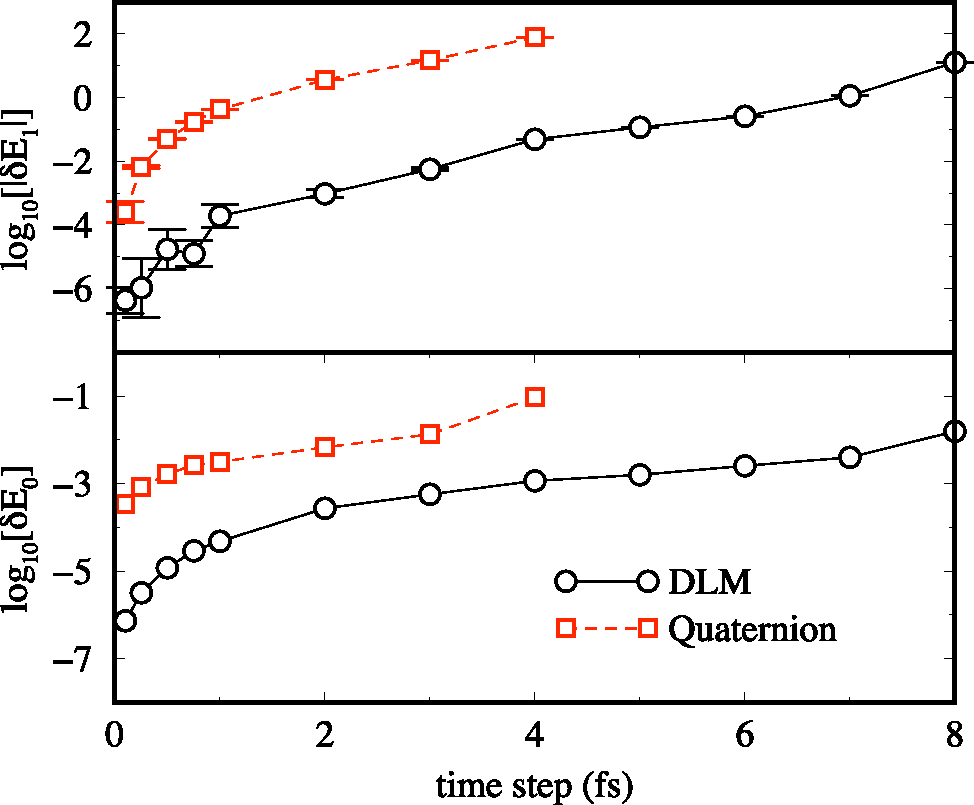
\includegraphics[width=\linewidth]{quatvsdlm.pdf}
\caption[Energy conservation analysis of the DLM and quaternion 
integration methods]{Analysis of the energy conservation of the DLM 
and quaternion integration methods.  $\delta \mathrm{E}_1$ is the
linear drift in energy over time and $\delta \mathrm{E}_0$ is the
standard deviation of energy fluctuations around this drift.  All
simulations were of a 1024-molecule simulation of SSD water at 298 K
starting from the same initial configuration. Note that the DLM
method provides more than an order of magnitude improvement in both
the energy drift and the size of the energy fluctuations when compared
with the quaternion method at any given time step.  At time steps
larger than 4 fs, the quaternion scheme resulted in rapidly rising
energies which eventually lead to simulation failure.  Using the DLM
method, time steps up to 8 fs can be taken before this behavior
is evident.}
\label{quatdlm}
\end{figure}

In Fig.~\ref{quatdlm}, $\delta \mbox{E}_1$ is a measure of the linear
energy drift in units of $\mbox{kcal mol}^{-1}$ per particle over a
nanosecond of simulation time, and $\delta \mbox{E}_0$ is the standard
deviation of the energy fluctuations in units of $\mbox{kcal
mol}^{-1}$ per particle. In the top plot, it is apparent that the
energy drift is reduced by a significant amount (2 to 3 orders of
magnitude improvement at all tested time steps) by chosing the DLM
method over the simple non-symplectic quaternion integration
method.  In addition to this improvement in energy drift, the
fluctuations in the total energy are also dampened by 1 to 2 orders of
magnitude by utilizing the DLM method.

Although the DLM method is more computationally expensive than
the traditional quaternion scheme for propagating a single time step,
consideration of the computational cost for a long simulation with a
particular level of energy conservation is in order.  A plot of energy
drift versus computational cost was generated
(Fig.~\ref{cpuCost}). This figure provides an estimate of the CPU time
required under the two integration schemes for 1 nanosecond of
simulation time for the model 1024-molecule system.  By chosing a
desired energy drift value it is possible to determine the CPU time
required for both methods. If a $\delta \mbox{E}_1$ of $1 \times
10^{-3} \mbox{kcal mol}^{-1}$ per particle is desired, a nanosecond of
simulation time will require ~19 hours of CPU time with the DLM
integrator, while the quaternion scheme will require ~154 hours of CPU
time. This demonstrates the computational advantage of the integration
scheme utilized in OpenMD.

\begin{figure}
\centering
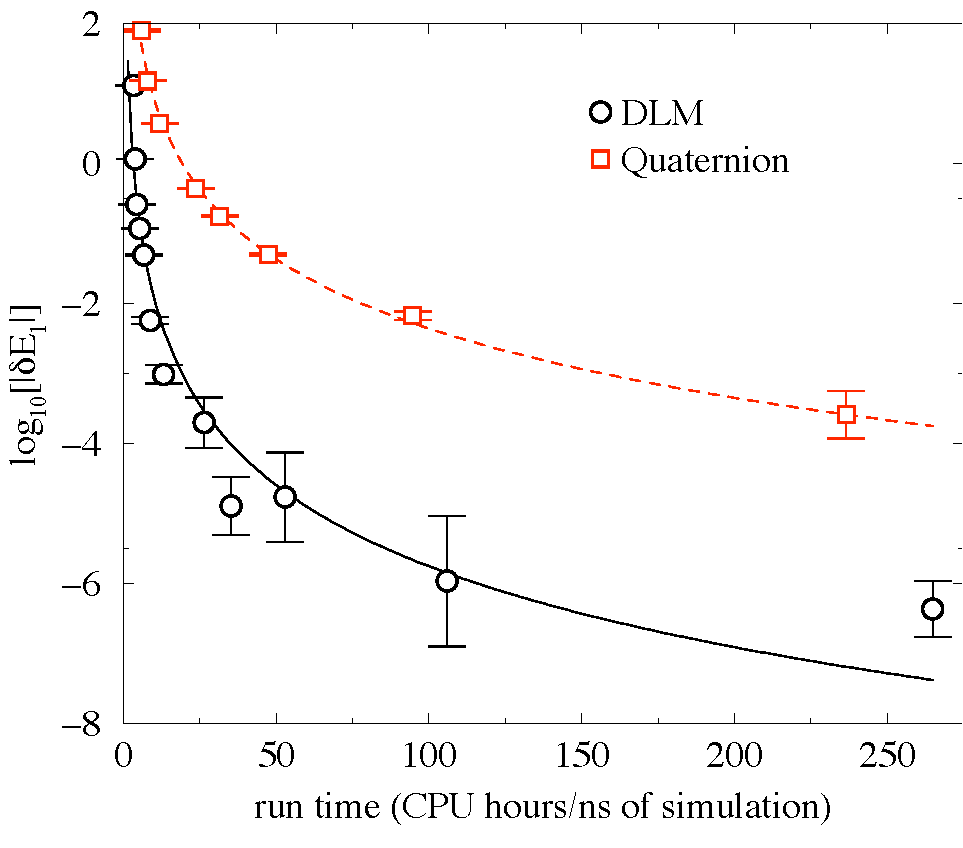
\includegraphics[width=\linewidth]{compCost.pdf}
\caption[Energy drift as a function of required simulation run 
time]{Energy drift as a function of required simulation run time.
$\delta \mathrm{E}_1$ is the linear drift in energy over time.
Simulations were performed on a single 2.5 GHz Pentium 4
processor. Simulation time comparisons can be made by tracing
horizontally from one curve to the other. For example, a simulation
that takes ~24 hours using the DLM method will take roughly 210
hours using the simple quaternion method if the same degree of energy
conservation is desired.}
\label{cpuCost}
\end{figure}

There is only one specific keyword relevant to the default integrator,
and that is the time step for integrating the equations of motion.

\begin{center}
\begin{tabular}{llll}
\textbf{variable} & \textbf{Meta-data keyword} & \textbf{units} &
                                                                  \textbf{default value} \\
$h$ & {\tt dt = 2.0;} & fs & none 
\end{tabular}
\end{center}

\section{\label{sec:extended}Extended Systems for other Ensembles}

OpenMD implements a number of extended system integrators for
sampling from other ensembles relevant to chemical physics.  The
integrator can be selected with the {\tt ensemble} keyword in the
meta-data file:

\begin{center}
\begin{tabular}{lll}
{\bf Integrator} & {\bf Ensemble} & {\bf Meta-data instruction} \\
NVE & microcanonical & {\tt ensemble = NVE; } \\
NVT & canonical & {\tt ensemble = NVT; } \\
NPTi & isobaric-isothermal & {\tt ensemble = NPTi;} \\
  &  (with isotropic volume changes) & \\
NPTf & isobaric-isothermal & {\tt ensemble = NPTf;} \\
  & (with changes to box shape) & \\
NPTxyz & approximate isobaric-isothermal & {\tt ensemble = NPTxyz;} \\
 &  (with separate barostats on each box dimension) & \\
N$\gamma$T & constant lateral surface tension & {\tt ensemble = NgammaT;} \\
 &  (must specify a surfaceTension) & \\
NP$\gamma$T & constant normal pressure and lateral surface tension & {\tt ensemble = NPrT;} \\
 &  (must specify a targetPressure and surfaceTension) & \\
LD & Langevin Dynamics & {\tt ensemble = LD;} \\
 &  (approximates the effects of an implicit solvent) & \\
 LangevinHull & Non-periodic Langevin Dynamics  & {\tt ensemble = LangevinHull;} \\
 & (Langevin Dynamics for molecules on convex hull;\\
 & Newtonian for interior molecules) & \\
\end{tabular}
\end{center}

These integrators allow the user to set target values for some
thermodynamic variables, they conserve others exactly, and allow some
conjugate property to float. For example, the {\tt NgammaT} integrator
has target values for pressure ($P$), temperature ($T$) and lateral
surface tension ($\gamma$).  It conserves particle number ($N$) and
the $z$-box dimension ($H_{zz}$), while allowing the energy ($E$), and
other box dimensions ($H_{xx}$, $H_{yy}$) to change.

\begin{longtable}{BAAA}
  \caption{Integrators implemented in OpenMD with their floating,
  target, and conserved Thermodynamic Quantities.} \\
  {\bf Integrator} & {\bf Floating Variables} & {\bf Target Variables} & {\bf Conserved Quantity}  \\ 
  \hline
\endhead
\hline
\endfoot
  NPA & E, T, H$_{zz}$ & P$_\mathrm{\hat{n}}$ & N, A$_{xy}$ \\
  NPAT & E, H$_{zz}$ & P$_\mathrm{\hat{n}}$, T & N,  A$_{xy}$ \\
  NPTf & E, $\overset\leftrightarrow{\mathrm{H}}$ & P, T& N, G \\
  NPTsz & E, H$_{zz}$, A$_{xy}$ & P, T & N \\
  NPTxyz & E, $\overset\leftrightarrow{\mathrm{H}}$ & P, T & N \\
  NPrT & E, $\overset\leftrightarrow{\mathrm{H}}$ & P$_\mathrm{\hat{n}}$, $\gamma$, T & N \\
  NgammaT & E, H$_{xx}$, H$_{yy}$ & P, T, $\gamma$ & N, $H_{zz}$\\
  NVT & E, P & T & N, V \\
  NVE & P, T & - & N, $\overset\leftrightarrow{\mathrm{H}}$, E \\
  LD & E & T & N, V \\
  LHull & E, V & P, T & N \\
\end{longtable}

The relatively well-known Nos\'e-Hoover thermostat\cite{Hoover85} is
implemented in OpenMD's NVT integrator.  This method couples an
extra degree of freedom (the thermostat) to the kinetic energy of the
system and it has been shown to sample the canonical distribution in
the system degrees of freedom while conserving a quantity that is, to
within a constant, the Helmholtz free energy.\cite{melchionna93}

NPT algorithms attempt to maintain constant pressure in the system by
coupling the volume of the system to a barostat.  OpenMD contains
three different constant pressure algorithms.  The first two, NPTi and
NPTf have been shown to conserve a quantity that is, to within a
constant, the Gibbs free energy.\cite{melchionna93} The Melchionna
modification to the Hoover barostat is implemented in both NPTi and
NPTf.  NPTi allows only isotropic changes in the simulation box, while
box {\it shape} variations are allowed in NPTf.  The NPTxyz integrator
has {\it not} been shown to sample from the isobaric-isothermal
ensemble.  It is useful, however, in that it maintains orthogonality
for the axes of the simulation box while attempting to equalize
pressure along the three perpendicular directions in the box.

Each of the extended system integrators requires additional keywords
to set target values for the thermodynamic state variables that are
being held constant.  Keywords are also required to set the
characteristic decay times for the dynamics of the extended
variables.

\begin{center}
\begin{tabular}{llll}
{\bf variable} & {\bf Meta-data instruction} & {\bf units} & {\bf
default value} \\  
$T_{\mathrm{target}}$ & {\tt targetTemperature = 300;} &  K & none \\
$P_{\mathrm{target}}$ & {\tt targetPressure = 1;} & atm & none \\
$\gamma$ & {\tt surfaceTension = 0.015;} & Newtons / meter & none \\
$\eta$ & {\tt viscosity = 0.0089;} & Poise & none \\
$\tau_T$ & {\tt tauThermostat = 1e3;} & fs & none \\
$\tau_B$ & {\tt tauBarostat = 5e3;} & fs  & none \\
         & {\tt resetTime = 200;} & fs & none \\
         & {\tt useInitialExtendedSystemState = true;} & logical &
true
\end{tabular}
\end{center}

Two additional keywords can be used to either clear the extended
system variables periodically ({\tt resetTime}), or to maintain the
state of the extended system variables between simulations ({\tt
useInitialExtendedSystemState}).  More details on these variables
and their use in the integrators follows below.

\section{\label{section:noseHooverThermo}Nos\'{e}-Hoover Thermostatting}

The Nos\'e-Hoover equations of motion are given by\cite{Hoover85}
\begin{eqnarray}
\dot{{\bf r}} & = & {\bf v}, \\
\dot{{\bf v}} & = & \frac{{\bf f}}{m} - \chi {\bf v} ,\\
\dot{\mathsf{A}} & = & \mathsf{A} \cdot
\mbox{ skew}\left(\overleftrightarrow{\mathsf{I}}^{-1} \cdot {\bf j}\right), \\
\dot{{\bf j}} & = & {\bf j} \times \left( \overleftrightarrow{\mathsf{I}}^{-1}
\cdot {\bf j} \right) - \mbox{ rot}\left(\mathsf{A}^{T} \cdot \frac{\partial
V}{\partial \mathsf{A}} \right) - \chi {\bf j}.
\label{eq:nosehoovereom}
\end{eqnarray}

$\chi$ is an ``extra'' variable included in the extended system, and
it is propagated using the first order equation of motion
\begin{equation}
\dot{\chi} = \frac{1}{\tau_{T}^2} \left( \frac{T}{T_{\mathrm{target}}} - 1 \right).
\label{eq:nosehooverext}
\end{equation}

The instantaneous temperature $T$ is proportional to the total kinetic
energy (both translational and orientational) and is given by
\begin{equation}
T = \frac{2 K}{f k_B}
\end{equation}
Here, $f$ is the total number of degrees of freedom in the system,
\begin{equation}
f = 3 N + 2 N_{\mathrm{linear}} + 3 N_{\mathrm{non-linear}} - N_{\mathrm{constraints}},
\end{equation}
and $K$ is the total kinetic energy,
\begin{equation}
K = \sum_{i=1}^{N} \frac{1}{2} m_i {\bf v}_i^T \cdot {\bf v}_i +
\sum_{i=1}^{N_{\mathrm{linear}}+N_{\mathrm{non-linear}}}  \frac{1}{2} {\bf j}_i^T \cdot
\overleftrightarrow{\mathsf{I}}_i^{-1} \cdot {\bf j}_i.
\end{equation}
$N_{\mathrm{linear}}$ is the number of linear rotors (i.e. with two
non-zero moments of inertia), and $N_{\mathrm{non-linear}}$ is the
number of non-linear rotors (i.e. with three non-zero moments of
inertia).  

In eq.(\ref{eq:nosehooverext}), $\tau_T$ is the time constant for
relaxation of the temperature to the target value.  To set values for
$\tau_T$ or $T_{\mathrm{target}}$ in a simulation, one would use the
{\tt tauThermostat} and {\tt targetTemperature} keywords in the
meta-data file.  The units for {\tt tauThermostat} are fs, and the
units for the {\tt targetTemperature} are degrees K.   The integration
of the equations of motion is carried out in a velocity-Verlet style 2
part algorithm:

{\tt moveA:}
\begin{align*}
T(t) &\leftarrow \left\{{\bf v}(t)\right\}, \left\{{\bf j}(t)\right\} ,\\
%
{\bf v}\left(t + h / 2\right)  &\leftarrow {\bf v}(t) 
	+ \frac{h}{2} \left( \frac{{\bf f}(t)}{m} - {\bf v}(t)
	\chi(t)\right), \\
%
{\bf r}(t + h) &\leftarrow {\bf r}(t) 
	+ h {\bf v}\left(t + h / 2 \right) ,\\
%
{\bf j}\left(t + h / 2 \right)  &\leftarrow {\bf j}(t) 
	+ \frac{h}{2} \left( {\bf \tau}^b(t) - {\bf j}(t)
	\chi(t) \right) ,\\
%
\mathsf{A}(t + h) &\leftarrow \mathrm{rotate}
	\left(h * {\bf j}(t + h / 2) 
	\overleftrightarrow{\mathsf{I}}^{-1} \right) ,\\
%
\chi\left(t + h / 2 \right) &\leftarrow \chi(t) 
	+ \frac{h}{2 \tau_T^2} \left( \frac{T(t)}
	{T_{\mathrm{target}}} - 1 \right) .
\end{align*}

Here $\mathrm{rotate}(h * {\bf j}
\overleftrightarrow{\mathsf{I}}^{-1})$ is the same symplectic Trotter
factorization of the three rotation operations that was discussed in
the section on the DLM integrator.  Note that this operation modifies
both the rotation matrix $\mathsf{A}$ and the angular momentum ${\bf
j}$.  {\tt moveA} propagates velocities by a half time step, and
positional degrees of freedom by a full time step.  The new positions
(and orientations) are then used to calculate a new set of forces and
torques in exactly the same way they are calculated in the {\tt
doForces} portion of the DLM integrator.

Once the forces and torques have been obtained at the new time step,
the temperature, velocities, and the extended system variable can be
advanced to the same time value.

{\tt moveB:}
\begin{align*}
T(t + h) &\leftarrow \left\{{\bf v}(t + h)\right\}, 
	\left\{{\bf j}(t + h)\right\}, \\
%
\chi\left(t + h \right) &\leftarrow \chi\left(t + h /
	2 \right) + \frac{h}{2 \tau_T^2} \left( \frac{T(t+h)}
	{T_{\mathrm{target}}} - 1 \right), \\
%
{\bf v}\left(t + h \right)  &\leftarrow {\bf v}\left(t 
	+ h / 2 \right) + \frac{h}{2} \left(
	\frac{{\bf f}(t + h)}{m} - {\bf v}(t + h)
	\chi(t h)\right) ,\\
%
{\bf j}\left(t + h \right) &\leftarrow {\bf j}\left(t
	+ h / 2 \right) + \frac{h}{2} 
	\left( {\bf \tau}^b(t + h) - {\bf j}(t + h) 
	\chi(t + h) \right) .
\end{align*}

Since ${\bf v}(t + h)$ and ${\bf j}(t + h)$ are required to calculate
$T(t + h)$ as well as $\chi(t + h)$, they indirectly depend on their
own values at time $t + h$.  {\tt moveB} is therefore done in an
iterative fashion until $\chi(t + h)$ becomes self-consistent.  The
relative tolerance for the self-consistency check defaults to a value
of $\mbox{10}^{-6}$, but OpenMD will terminate the iteration
after 4 loops even if the consistency check has not been satisfied.

The Nos\'e-Hoover algorithm is known to conserve a Hamiltonian for the
extended system that is, to within a constant, identical to the
Helmholtz free energy,\cite{melchionna93}
\begin{equation}
H_{\mathrm{NVT}} = V + K + f k_B T_{\mathrm{target}} \left(
\frac{\tau_{T}^2 \chi^2(t)}{2} + \int_{0}^{t} \chi(t^\prime) dt^\prime
\right).
\end{equation}
Poor choices of $h$ or $\tau_T$ can result in non-conservation
of $H_{\mathrm{NVT}}$, so the conserved quantity is maintained in the
last column of the {\tt .stat} file to allow checks on the quality of
the integration.

Bond constraints are applied at the end of both the {\tt moveA} and
{\tt moveB} portions of the algorithm.  Details on the constraint
algorithms are given in section \ref{section:rattle}.

\section{\label{sec:NPTi}Constant-pressure integration with 
isotropic box deformations (NPTi)}

To carry out isobaric-isothermal ensemble calculations, OpenMD
implements the Melchionna modifications to the Nos\'e-Hoover-Andersen
equations of motion.\cite{melchionna93} The equations of motion are
the same as NVT with the following exceptions:

\begin{eqnarray}
\dot{{\bf r}} & = & {\bf v} + \eta \left( {\bf r} - {\bf R}_0 \right), \\
\dot{{\bf v}} & = & \frac{{\bf f}}{m} - (\eta + \chi) {\bf v}, \\
\dot{\eta} & = & \frac{1}{\tau_{B}^2 f k_B T_{\mathrm{target}}} V \left( P -
P_{\mathrm{target}} \right), \\
\dot{\mathcal{V}} & = & 3 \mathcal{V} \eta .
\label{eq:melchionna1}
\end{eqnarray}

$\chi$ and $\eta$ are the ``extra'' degrees of freedom in the extended
system.  $\chi$ is a thermostat, and it has the same function as it
does in the Nos\'e-Hoover NVT integrator.  $\eta$ is a barostat which
controls changes to the volume of the simulation box.  ${\bf R}_0$ is
the location of the center of mass for the entire system, and
$\mathcal{V}$ is the volume of the simulation box.  At any time, the
volume can be calculated from the determinant of the matrix which
describes the box shape:
\begin{equation}
\mathcal{V} = \det(\mathsf{H}).
\end{equation}

The NPTi integrator requires an instantaneous pressure. This quantity
is calculated via the pressure tensor,
\begin{equation}
\overleftrightarrow{\mathsf{P}}(t) = \frac{1}{\mathcal{V}(t)} \left(
\sum_{i=1}^{N} m_i {\bf v}_i(t) \otimes {\bf v}_i(t) +
\overleftrightarrow{\mathsf{W}}(t) \right).
\end{equation}
The kinetic contribution to the pressure tensor utilizes the {\it
outer} product of the velocities, denoted by the $\otimes$ symbol.  The
virial tensor is calculated from another outer product of the
inter-atomic separation vectors (${\bf r}_{ij} = {\bf r}_j - {\bf
r}_i$) with the forces between the same two atoms,
\begin{equation}
\overleftrightarrow{\mathsf{W}}(t) = \sum_{i} \sum_{j>i} {\bf r}_{ij}(t)
\otimes {\bf f}_{ij}(t).
\end{equation}
In systems containing cutoff groups, the virial tensor is computed
between the centers-of-mass of the cutoff groups:
\begin{equation}
\overleftrightarrow{\mathsf{W}}(t) = \sum_{a} \sum_{b} {\bf r}_{ab}(t)
\otimes {\bf f}_{ab}(t).
\end{equation}
where ${\bf r}_{ab}$ is the distance between the centers of mass, and 
\begin{equation}
{\bf f}_{ab} = s(r_{ab}) \sum_{i \in a} \sum_{j \in b} {\bf f}_{ij} +
s^{\prime}(r_{ab}) \frac{{\bf r}_{ab}}{|r_{ab}|} \sum_{i \in a} \sum_{j
\in b} V_{ij}({\bf r}_{ij}).
\end{equation}

The instantaneous pressure is then simply obtained from the trace of
the pressure tensor,
\begin{equation}
P(t) = \frac{1}{3} \mathrm{Tr} \left( \overleftrightarrow{\mathsf{P}}(t)
\right).
\end{equation}

In eq.(\ref{eq:melchionna1}), $\tau_B$ is the time constant for
relaxation of the pressure to the target value.  To set values for
$\tau_B$ or $P_{\mathrm{target}}$ in a simulation, one would use the
{\tt tauBarostat} and {\tt targetPressure} keywords in the meta-data
file.  The units for {\tt tauBarostat} are fs, and the units for the
{\tt targetPressure} are atmospheres.  Like in the NVT integrator, the
integration of the equations of motion is carried out in a
velocity-Verlet style two part algorithm with only the following
differences:

{\tt moveA:}
\begin{align*}
P(t) &\leftarrow \left\{{\bf r}(t)\right\}, \left\{{\bf v}(t)\right\} ,\\
%
{\bf v}\left(t + h / 2\right)  &\leftarrow {\bf v}(t) 
	+ \frac{h}{2} \left( \frac{{\bf f}(t)}{m} - {\bf v}(t)
	\left(\chi(t) + \eta(t) \right) \right), \\
%
\eta(t + h / 2) &\leftarrow \eta(t) + \frac{h 
	\mathcal{V}(t)}{2 N k_B T(t) \tau_B^2} \left( P(t) 
	- P_{\mathrm{target}} \right), \\ 
%
{\bf r}(t + h) &\leftarrow {\bf r}(t) + h 
	\left\{ {\bf v}\left(t + h / 2 \right) 
	+ \eta(t + h / 2)\left[ {\bf r}(t + h) 
	- {\bf R}_0 \right] \right\} ,\\
%
\mathsf{H}(t + h) &\leftarrow e^{-h \eta(t + h / 2)} 
	\mathsf{H}(t).
\end{align*}

The propagation of positions to time $t + h$
depends on the positions at the same time.  OpenMD carries out
this step iteratively (with a limit of 5 passes through the iterative
loop).  Also, the simulation box $\mathsf{H}$ is scaled uniformly for
one full time step by an exponential factor that depends on the value
of $\eta$ at time $t +
h / 2$.  Reshaping the box uniformly also scales the volume of
the box by
\begin{equation}
\mathcal{V}(t + h) \leftarrow e^{ - 3 h \eta(t + h /2)} \times
\mathcal{V}(t).
\end{equation}

The {\tt doForces} step for the NPTi integrator is exactly the same as
in both the DLM and NVT integrators.  Once the forces and torques have
been obtained at the new time step, the velocities can be advanced to
the same time value.

{\tt moveB:}
\begin{align*}
P(t + h) &\leftarrow  \left\{{\bf r}(t + h)\right\},
	\left\{{\bf v}(t + h)\right\}, \\
%
\eta(t + h) &\leftarrow \eta(t + h / 2) +
	\frac{h \mathcal{V}(t + h)}{2 N k_B T(t + h) 
	\tau_B^2} \left( P(t + h) - P_{\mathrm{target}} \right), \\ 
%
{\bf v}\left(t + h \right)  &\leftarrow {\bf v}\left(t 
	+ h / 2 \right) + \frac{h}{2} \left(
	\frac{{\bf f}(t + h)}{m} - {\bf v}(t + h)
	(\chi(t + h) + \eta(t + h)) \right) ,\\
%
{\bf j}\left(t + h \right)  &\leftarrow {\bf j}\left(t 
	+ h / 2 \right) + \frac{h}{2} \left( {\bf
	\tau}^b(t + h) - {\bf j}(t + h)
	\chi(t + h) \right) .
\end{align*}

Once again, since ${\bf v}(t + h)$ and ${\bf j}(t + h)$ are required
to calculate $T(t + h)$, $P(t + h)$, $\chi(t + h)$, and $\eta(t +
h)$, they indirectly depend on their own values at time $t + h$.  {\tt
moveB} is therefore done in an iterative fashion until $\chi(t + h)$
and $\eta(t + h)$ become self-consistent.  The relative tolerance for
the self-consistency check defaults to a value of $\mbox{10}^{-6}$,
but OpenMD will terminate the iteration after 4 loops even if the
consistency check has not been satisfied.

The Melchionna modification of the Nos\'e-Hoover-Andersen algorithm is
known to conserve a Hamiltonian for the extended system that is, to
within a constant, identical to the Gibbs free energy,
\begin{equation}
H_{\mathrm{NPTi}} = V + K + f k_B T_{\mathrm{target}} \left(
\frac{\tau_{T}^2 \chi^2(t)}{2} + \int_{0}^{t} \chi(t^\prime) dt^\prime
\right) + P_{\mathrm{target}} \mathcal{V}(t).
\end{equation}
Poor choices of $\delta t$, $\tau_T$, or $\tau_B$ can result in
non-conservation of $H_{\mathrm{NPTi}}$, so the conserved quantity is
maintained in the last column of the {\tt .stat} file to allow checks
on the quality of the integration.  It is also known that this
algorithm samples the equilibrium distribution for the enthalpy
(including contributions for the thermostat and barostat), 
\begin{equation}
H_{\mathrm{NPTi}} = V + K + \frac{f k_B T_{\mathrm{target}}}{2} \left(
\chi^2 \tau_T^2 + \eta^2 \tau_B^2 \right) +  P_{\mathrm{target}}
\mathcal{V}(t). 
\end{equation}

Bond constraints are applied at the end of both the {\tt moveA} and
{\tt moveB} portions of the algorithm.  Details on the constraint
algorithms are given in section \ref{section:rattle}.

\section{\label{sec:NPTf}Constant-pressure integration with a
flexible box (NPTf)} 

There is a relatively simple generalization of the
Nos\'e-Hoover-Andersen method to include changes in the simulation box
{\it shape} as well as in the volume of the box.  This method utilizes
the full $3 \times 3$ pressure tensor and introduces a tensor of
extended variables ($\overleftrightarrow{\eta}$) to control changes to
the box shape.  The equations of motion for this method differ from
those of NPTi as follows:
\begin{eqnarray}
\dot{{\bf r}} & = & {\bf v} + \overleftrightarrow{\eta} \cdot \left( {\bf r} - {\bf R}_0 \right), \\
\dot{{\bf v}} & = & \frac{{\bf f}}{m} - (\overleftrightarrow{\eta} +
\chi \cdot \mathsf{1}) {\bf v}, \\
\dot{\overleftrightarrow{\eta}} & = & \frac{1}{\tau_{B}^2 f k_B
T_{\mathrm{target}}} V \left( \overleftrightarrow{\mathsf{P}} - P_{\mathrm{target}}\mathsf{1} \right) ,\\
\dot{\mathsf{H}} & = &  \overleftrightarrow{\eta} \cdot \mathsf{H} .
\label{eq:melchionna2}
\end{eqnarray}

Here, $\mathsf{1}$ is the unit matrix and $\overleftrightarrow{\mathsf{P}}$
is the pressure tensor.  Again, the volume, $\mathcal{V} = \det
\mathsf{H}$. 

The propagation of the equations of motion is nearly identical to the
NPTi integration:

{\tt moveA:}
\begin{align*}
\overleftrightarrow{\mathsf{P}}(t) &\leftarrow \left\{{\bf r}(t)\right\}, 
	\left\{{\bf v}(t)\right\} ,\\
%
{\bf v}\left(t + h / 2\right)  &\leftarrow {\bf v}(t) 
	+ \frac{h}{2} \left( \frac{{\bf f}(t)}{m} - 
	\left(\chi(t)\mathsf{1} + \overleftrightarrow{\eta}(t) \right) \cdot
	{\bf v}(t) \right), \\ 
%
\overleftrightarrow{\eta}(t + h / 2) &\leftarrow 
	\overleftrightarrow{\eta}(t) + \frac{h \mathcal{V}(t)}{2 N k_B
	T(t) \tau_B^2} \left( \overleftrightarrow{\mathsf{P}}(t) 
	- P_{\mathrm{target}}\mathsf{1} \right), \\ 
%
{\bf r}(t + h) &\leftarrow {\bf r}(t) + h \left\{ {\bf v}
	\left(t + h / 2 \right) + \overleftrightarrow{\eta}(t +
	h / 2) \cdot \left[ {\bf r}(t + h) 
	- {\bf R}_0 \right] \right\}, \\
%
\mathsf{H}(t + h) &\leftarrow \mathsf{H}(t) \cdot e^{-h
	\overleftrightarrow{\eta}(t + h / 2)} .
\end{align*}
OpenMD uses a power series expansion truncated at second order
for the exponential operation which scales the simulation box.

The {\tt moveB} portion of the algorithm is largely unchanged from the
NPTi integrator:

{\tt moveB:}
\begin{align*}
\overleftrightarrow{\mathsf{P}}(t + h) &\leftarrow \left\{{\bf r}
	(t + h)\right\}, \left\{{\bf v}(t 
	+ h)\right\}, \left\{{\bf f}(t + h)\right\} ,\\
%
\overleftrightarrow{\eta}(t + h) &\leftarrow 
	\overleftrightarrow{\eta}(t + h / 2) +
	\frac{h \mathcal{V}(t + h)}{2 N k_B T(t + h) 
	\tau_B^2} \left( \overleftrightarrow{P}(t + h) 
	- P_{\mathrm{target}}\mathsf{1} \right) ,\\ 
%
{\bf v}\left(t + h \right)  &\leftarrow {\bf v}\left(t 
	+ h / 2 \right) + \frac{h}{2} \left(
	\frac{{\bf f}(t + h)}{m} - 
	(\chi(t + h)\mathsf{1} + \overleftrightarrow{\eta}(t 
	+ h)) \right) \cdot {\bf v}(t + h), \\
\end{align*}

The iterative schemes for both {\tt moveA} and {\tt moveB} are
identical to those described for the NPTi integrator.

The NPTf integrator is known to conserve the following Hamiltonian:
\begin{equation}
H_{\mathrm{NPTf}} = V + K + f k_B T_{\mathrm{target}} \left(
\frac{\tau_{T}^2 \chi^2(t)}{2} + \int_{0}^{t} \chi(t^\prime) dt^\prime
\right) + P_{\mathrm{target}} \mathcal{V}(t) + \frac{f k_B
T_{\mathrm{target}}}{2}
\mathrm{Tr}\left[\overleftrightarrow{\eta}(t)\right]^2 \tau_B^2.
\end{equation}

This integrator must be used with care, particularly in liquid
simulations.  Liquids have very small restoring forces in the
off-diagonal directions, and the simulation box can very quickly form
elongated and sheared geometries which become smaller than the cutoff
radius.  The NPTf integrator finds most use in simulating crystals or
liquid crystals which assume non-orthorhombic geometries.

\section{\label{nptxyz}Constant pressure in 3 axes (NPTxyz)}

There is one additional extended system integrator which is somewhat
simpler than the NPTf method described above.  In this case, the three
axes have independent barostats which each attempt to preserve the
target pressure along the box walls perpendicular to that particular
axis.  The lengths of the box axes are allowed to fluctuate
independently, but the angle between the box axes does not change.
The equations of motion are identical to those described above, but
only the {\it diagonal} elements of $\overleftrightarrow{\eta}$ are
computed.  The off-diagonal elements are set to zero (even when the
pressure tensor has non-zero off-diagonal elements).

It should be noted that the NPTxyz integrator is {\it not} known to
preserve any Hamiltonian of interest to the chemical physics
community.  The integrator is extremely useful, however, in generating
initial conditions for other integration methods.  It {\it is} suitable
for use with liquid simulations, or in cases where there is
orientational anisotropy in the system (i.e. in lipid bilayer
simulations).

\section{Langevin Dynamics (LD)\label{LDRB}}

OpenMD implements a Langevin integrator in order to perform
molecular dynamics simulations in implicit solvent environments.  This
can result in substantial performance gains when the detailed dynamics
of the solvent is not important. Since OpenMD also handles rigid
bodies of arbitrary composition and shape, the Langevin integrator is
by necessity somewhat more complex than in other simulation packages.

Consider the Langevin equations of motion in generalized coordinates
\begin{equation}
{\bf M} \dot{{\bf V}}(t) = {\bf F}_{s}(t) +
{\bf F}_{f}(t)  + {\bf F}_{r}(t) 
\label{LDGeneralizedForm}
\end{equation}
where ${\bf M}$ is a $6 \times 6$ diagonal mass matrix (which
includes the mass of the rigid body as well as the moments of inertia
in the body-fixed frame) and ${\bf V}$ is a generalized velocity,
${\bf V} =
\left\{{\bf v},{\bf \omega}\right\}$. The right side of
Eq. \ref{LDGeneralizedForm} consists of three generalized forces: a
system force (${\bf F}_{s}$), a frictional or dissipative force (${\bf
F}_{f}$) and a stochastic force (${\bf F}_{r}$). While the evolution
of the system in Newtonian mechanics is typically done in the lab
frame, it is convenient to handle the dynamics of rigid bodies in
body-fixed frames. Thus the friction and random forces on each
substructure are calculated in a body-fixed frame and may converted
back to the lab frame using that substructure's rotation matrix (${\bf
Q}$):
\begin{equation}
{\bf F}_{f,r} = 
\left( \begin{array}{c}
{\bf f}_{f,r} \\
{\bf \tau}_{f,r}
\end{array} \right)
=
\left( \begin{array}{c}
{\bf Q}^{T} {\bf f}^{~b}_{f,r} \\
{\bf Q}^{T} {\bf \tau}^{~b}_{f,r}
\end{array} \right)
\end{equation}
The body-fixed friction force, ${\bf F}_{f}^{~b}$, is proportional to
the (body-fixed) velocity at the center of resistance
${\bf v}_{R}^{~b}$ and the angular velocity ${\bf \omega}$
\begin{equation}
{\bf F}_{f}^{~b}(t) = \left( \begin{array}{l}
 {\bf f}_{f}^{~b}(t) \\
 {\bf \tau}_{f}^{~b}(t) \\
 \end{array} \right) =  - \left( \begin{array}{*{20}c}
   \Xi_{R}^{tt} & \Xi_{R}^{rt} \\
   \Xi_{R}^{tr} & \Xi_{R}^{rr}    \\
\end{array} \right)\left( \begin{array}{l}
 {\bf v}_{R}^{~b}(t) \\
 {\bf \omega}(t) \\
 \end{array} \right),
\end{equation}
while the random force, ${\bf F}_{r}$, is a Gaussian stochastic
variable with zero mean and variance,
\begin{equation}
\left\langle {{\bf F}_{r}(t) ({\bf F}_{r}(t'))^T } \right\rangle  =
\left\langle {{\bf F}_{r}^{~b} (t) ({\bf F}_{r}^{~b} (t'))^T } \right\rangle  =
2 k_B T \Xi_R \delta(t - t'). \label{eq:randomForce}
\end{equation}
$\Xi_R$ is the $6\times6$ resistance tensor at the center of
resistance.  

For atoms and ellipsoids, there are good approximations for this
tensor that are based on Stokes' law.  For arbitrary rigid bodies, the
resistance tensor must be pre-computed before Langevin dynamics can be
used.  The OpenMD distribution contains a utitilty program called
Hydro that performs this computation.

Once this tensor is known for a given {\tt integrableObject},
obtaining a stochastic vector that has the properties in
Eq. (\ref{eq:randomForce}) can be done efficiently by carrying out a
one-time Cholesky decomposition to obtain the square root matrix of
the resistance tensor,
\begin{equation} 
\Xi_R = {\bf S} {\bf S}^{T},
\label{eq:Cholesky}
\end{equation} 
where ${\bf S}$ is a lower triangular matrix.\cite{Schlick2002} A
vector with the statistics required for the random force can then be
obtained by multiplying ${\bf S}$ onto a random 6-vector ${\bf Z}$ which
has elements chosen from a Gaussian distribution, such that:
\begin{equation}
\langle {\bf Z}_i \rangle = 0, \hspace{1in} \langle {\bf Z}_i \cdot
{\bf Z}_j \rangle = \frac{2 k_B T}{\delta t} \delta_{ij},
\end{equation}
where $\delta t$ is the timestep in use during the simulation. The
random force, ${\bf F}_{r}^{~b} = {\bf S} {\bf Z}$, can be shown to have the
correct properties required by Eq. (\ref{eq:randomForce}).

The equation of motion for the translational velocity of the center of
mass (${\bf v}$) can be written as
\begin{equation}
m \dot{{\bf v}} (t) =  {\bf f}_{s}(t) + {\bf f}_{f}(t) +
{\bf f}_{r}(t)
\end{equation}
Since the frictional and random forces are applied at the center of
resistance, which generally does not coincide with the center of mass,
extra torques are exerted at the center of mass. Thus, the net
body-fixed torque at the center of mass, $\tau^{~b}(t)$,
is given by
\begin{equation}
\tau^{~b} \leftarrow \tau_{s}^{~b} + \tau_{f}^{~b} + \tau_{r}^{~b} + {\bf r}_{MR} \times \left( {\bf f}_{f}^{~b} + {\bf f}_{r}^{~b} \right)
\end{equation}
where ${\bf r}_{MR}$ is the vector from the center of mass to the center of
resistance. Instead of integrating the angular velocity in lab-fixed
frame, we consider the equation of motion for the angular momentum
(${\bf j}$) in the body-fixed frame
\begin{equation}
\frac{\partial}{\partial t}{\bf j}(t) = \tau^{~b}(t)
\end{equation}
By embedding the friction and random forces into the the total force
and torque, OpenMD integrates the Langevin equations of motion
for a rigid body of arbitrary shape in a velocity-Verlet style 2-part
algorithm, where $h = \delta t$:

{\tt move A:}
\begin{align*}
{\bf v}\left(t + h / 2\right)  &\leftarrow  {\bf v}(t)
    + \frac{h}{2} \left( {\bf f}(t) / m \right), \\
%
{\bf r}(t + h) &\leftarrow {\bf r}(t)
    + h  {\bf v}\left(t + h / 2 \right), \\
%
{\bf j}\left(t + h / 2 \right)  &\leftarrow {\bf j}(t)
    + \frac{h}{2} {\bf \tau}^{~b}(t), \\
%
{\bf Q}(t + h) &\leftarrow \mathrm{rotate}\left( h {\bf j}
    (t + h / 2) \cdot \overleftrightarrow{\mathsf{I}}^{-1} \right).
\end{align*}
In this context, $\overleftrightarrow{\mathsf{I}}$ is the diagonal
moment of inertia tensor, and the $\mathrm{rotate}$ function is the
reversible product of the three body-fixed rotations,
\begin{equation}
\mathrm{rotate}({\bf a}) = \mathsf{G}_x(a_x / 2) \cdot
\mathsf{G}_y(a_y / 2) \cdot \mathsf{G}_z(a_z) \cdot \mathsf{G}_y(a_y
/ 2) \cdot \mathsf{G}_x(a_x /2),
\end{equation}
where each rotational propagator, $\mathsf{G}_\alpha(\theta)$,
rotates both the rotation matrix ($\mathbf{Q}$) and the body-fixed
angular momentum (${\bf j}$) by an angle $\theta$ around body-fixed
axis $\alpha$,
\begin{equation}
\mathsf{G}_\alpha( \theta ) = \left\{
\begin{array}{lcl}
\mathbf{Q}(t) & \leftarrow & \mathbf{Q}(0) \cdot \mathsf{R}_\alpha(\theta)^T, \\
{\bf j}(t) & \leftarrow & \mathsf{R}_\alpha(\theta) \cdot {\bf
j}(0).
\end{array}
\right.
\end{equation}
$\mathsf{R}_\alpha$ is a quadratic approximation to the single-axis
rotation matrix.  For example, in the small-angle limit, the
rotation matrix around the body-fixed x-axis can be approximated as
\begin{equation}
\mathsf{R}_x(\theta) \approx \left(
\begin{array}{ccc}
1 & 0 & 0 \\
0 & \frac{1-\theta^2 / 4}{1 + \theta^2 / 4}  & -\frac{\theta}{1+
\theta^2 / 4} \\
0 & \frac{\theta}{1+ \theta^2 / 4} & \frac{1-\theta^2 / 4}{1 +
\theta^2 / 4}
\end{array}
\right).
\end{equation}
All other rotations follow in a straightforward manner. After the
first part of the propagation, the forces and body-fixed torques are
calculated at the new positions and orientations.  The system forces
and torques are derivatives of the total potential energy function
($U$) with respect to the rigid body positions (${\bf r}$) and the
columns of the transposed rotation matrix ${\bf Q}^T = \left({\bf
u}_x, {\bf u}_y, {\bf u}_z \right)$:

{\tt Forces:}
\begin{align*}
{\bf f}_{s}(t + h) & \leftarrow
    - \left(\frac{\partial U}{\partial {\bf r}}\right)_{{\bf r}(t + h)} \\
%
{\bf \tau}_{s}(t + h) &\leftarrow {\bf u}(t + h)
    \times \frac{\partial U}{\partial {\bf u}} \\
%
{\bf v}^{b}_{R}(t+h) & \leftarrow \mathbf{Q}(t+h) \cdot \left({\bf v}(t+h) + {\bf \omega}(t+h) \times {\bf r}_{MR} \right) \\
%
{\bf f}_{R,f}^{b}(t+h) & \leftarrow - \Xi_{R}^{tt} \cdot
{\bf v}^{b}_{R}(t+h) - \Xi_{R}^{rt} \cdot {\bf \omega}(t+h) \\
%
{\bf \tau}_{R,f}^{b}(t+h) & \leftarrow - \Xi_{R}^{tr} \cdot
{\bf v}^{b}_{R}(t+h) - \Xi_{R}^{rr} \cdot {\bf \omega}(t+h) \\
%
Z & \leftarrow  {\tt GaussianNormal}(2 k_B T / h, 6) \\
{\bf F}_{R,r}^{b}(t+h) & \leftarrow {\bf S} \cdot Z \\
%
{\bf f}(t+h) & \leftarrow {\bf f}_{s}(t+h) + \mathbf{Q}^{T}(t+h)
\cdot \left({\bf f}_{R,f}^{~b} + {\bf f}_{R,r}^{~b} \right) \\
%
\tau(t+h) & \leftarrow \tau_{s}(t+h) + \mathbf{Q}^{T}(t+h) \cdot \left(\tau_{R,f}^{~b} + \tau_{R,r}^{~b} \right) + {\bf r}_{MR} \times \left({\bf f}_{f}(t+h) + {\bf f}_{r}(t+h) \right) \\
\tau^{~b}(t+h) & \leftarrow \mathbf{Q}(t+h) \cdot \tau(t+h) \\
\end{align*}
Frictional (and random) forces and torques must be computed at the
center of resistance, so there are additional steps required to find
the body-fixed velocity (${\bf v}_{R}^{~b}$) at this location.  Mapping
the frictional and random forces at the center of resistance back to
the center of mass also introduces an additional term in the torque
one obtains at the center of mass.

Once the forces and torques have been obtained at the new time step,
the velocities can be advanced to the same time value.

{\tt move B:}
\begin{align*}
{\bf v}\left(t + h \right)  &\leftarrow  {\bf v}\left(t + h / 2
\right)
    + \frac{h}{2} \left( {\bf f}(t + h) / m \right), \\
%
{\bf j}\left(t + h \right)  &\leftarrow {\bf j}\left(t + h / 2
\right)
    + \frac{h}{2} {\bf \tau}^{~b}(t + h) .
\end{align*}

The viscosity of the implicit solvent must be specified using the {\tt
viscosity} keyword in the meta-data file if the Langevin integrator is
selected. For simple particles (spheres and ellipsoids), no further
parameters are necessary.  Since there are no analytic solutions for
the resistance tensors for composite rigid bodies, the approximate
tensors for these objects must also be specified in order to use
Langevin dynamics.  The meta-data file must therefore point to another
file which contains the information about the hydrodynamic properties
of all complex rigid bodies being used during the simulation.  The
{\tt HydroPropFile} keyword is used to specify the name of this
file. A {\tt HydroPropFile} should be precalculated using the Hydro
program that is included in the OpenMD distribution.

\begin{longtable}[c]{ABG}
\caption{Meta-data Keywords: Required parameters for the Langevin integrator}
\\
{\bf keyword} & {\bf units} & {\bf use}  \\ \hline
\endhead
\hline
\endfoot
{\tt viscosity} & poise & Sets the value of viscosity of the implicit
solvent  \\ 
{\tt targetTemp} & K & Sets the target temperature of the system.
This parameter must be specified to use Langevin dynamics. \\ 
{\tt HydroPropFile} & string & Specifies the name of the resistance
tensor (usually a {\tt .hydro} file) which is precalculated by {\tt
Hydro}. This keyword is not necessary if the simulation contains only
simple bodies (spheres and ellipsoids). \\ 
\label{table:ldParameters}
\end{longtable}

\section{Constant Pressure without periodic boundary conditions (The LangevinHull)}

The Langevin Hull\cite{Vardeman2011} uses an external bath at a fixed constant pressure
($P$) and temperature ($T$) with an effective solvent viscosity
($\eta$).  This bath interacts only with the objects on the exterior
hull of the system.  Defining the hull of the atoms in a simulation is
done in a manner similar to the approach of Kohanoff, Caro and
Finnis.\cite{Kohanoff:2005qm} That is, any instantaneous configuration
of the atoms in the system is considered as a point cloud in three
dimensional space.  Delaunay triangulation is used to find all facets
between coplanar
neighbors.\cite{delaunay,springerlink:10.1007/BF00977785} In highly
symmetric point clouds, facets can contain many atoms, but in all but
the most symmetric of cases, the facets are simple triangles in
3-space which contain exactly three atoms.

The convex hull is the set of facets that have {\it no concave
  corners} at an atomic site.\cite{Barber96,EDELSBRUNNER:1994oq} This
eliminates all facets on the interior of the point cloud, leaving only
those exposed to the bath. Sites on the convex hull are dynamic; as
molecules re-enter the cluster, all interactions between atoms on that
molecule and the external bath are removed.  Since the edge is
determined dynamically as the simulation progresses, no {\it a priori}
geometry is defined. The pressure and temperature bath interacts only
with the atoms on the edge and not with atoms interior to the
simulation.

Atomic sites in the interior of the simulation move under standard
Newtonian dynamics,
\begin{equation}
m_i \dot{\mathbf v}_i(t)=-{\mathbf \nabla}_i U,
\label{eq:Newton}
\end{equation}
where $m_i$ is the mass of site $i$, ${\mathbf v}_i(t)$ is the
instantaneous velocity of site $i$ at time $t$, and $U$ is the total
potential energy.  For atoms on the exterior of the cluster
(i.e. those that occupy one of the vertices of the convex hull), the
equation of motion is modified with an external force, ${\mathbf
  F}_i^{\mathrm ext}$:
\begin{equation}
m_i \dot{\mathbf v}_i(t)=-{\mathbf \nabla}_i U + {\mathbf F}_i^{\mathrm ext}.
\end{equation}

The external bath interacts indirectly with the atomic sites through
the intermediary of the hull facets.  Since each vertex (or atom)
provides one corner of a triangular facet, the force on the facets are
divided equally to each vertex.  However, each vertex can participate
in multiple facets, so the resultant force is a sum over all facets
$f$ containing vertex $i$:
\begin{equation}
{\mathbf F}_{i}^{\mathrm ext} = \sum_{\begin{array}{c}\mathrm{facets\
    } f \\ \mathrm{containing\ } i\end{array}} \frac{1}{3}\  {\mathbf
  F}_f^{\mathrm ext}
\end{equation}

The external pressure bath applies a force to the facets of the convex
hull in direct proportion to the area of the facet, while the thermal
coupling depends on the solvent temperature, viscosity and the size
and shape of each facet. The thermal interactions are expressed as a
standard Langevin description of the forces,
\begin{equation}
\begin{array}{rclclcl}
{\mathbf F}_f^{\text{ext}} & = &  \text{external pressure} & + & \text{drag force} & + & \text{random force} \\
& = &  -\hat{n}_f P A_f  & - & \Xi_f(t) {\mathbf v}_f(t)  & + & {\mathbf R}_f(t)
\end{array}
\end{equation}
Here, $A_f$ and $\hat{n}_f$ are the area and (outward-facing) normal
vectors for facet $f$, respectively.  ${\mathbf v}_f(t)$ is the
velocity of the facet centroid,
\begin{equation}
{\mathbf v}_f(t) =  \frac{1}{3} \sum_{i=1}^{3} {\mathbf v}_i,
\end{equation}
and $\Xi_f(t)$ is an approximate ($3 \times 3$) resistance tensor that
depends on the geometry and surface area of facet $f$ and the
viscosity of the bath.  The resistance tensor is related to the
fluctuations of the random force, $\mathbf{R}(t)$, by the
fluctuation-dissipation theorem (see Eq. \ref{eq:randomForce}).

Once the resistance tensor is known for a given facet, a stochastic
vector that has the properties in Eq. (\ref{eq:randomForce}) can be
calculated efficiently by carrying out a Cholesky decomposition to
obtain the square root matrix of the resistance tensor (see
Eq. \ref{eq:Cholesky}).

Our treatment of the resistance tensor for the Langevin Hull facets is
approximate.  $\Xi_f$ for a rigid triangular plate would normally be
treated as a $6 \times 6$ tensor that includes translational and
rotational drag as well as translational-rotational coupling. The
computation of resistance tensors for rigid bodies has been detailed
elsewhere,\cite{JoseGarciadelaTorre02012000,Garcia-de-la-Torre:2001wd,GarciadelaTorreJ2002,Sun:2008fk}
but the standard approach involving bead approximations would be
prohibitively expensive if it were recomputed at each step in a
molecular dynamics simulation.

Instead, we are utilizing an approximate resistance tensor obtained by
first constructing the Oseen tensor for the interaction of the
centroid of the facet ($f$) with each of the subfacets $\ell=1,2,3$,
\begin{equation}
T_{\ell f}=\frac{A_\ell}{8\pi\eta R_{\ell f}}\left(I +
  \frac{\mathbf{R}_{\ell f}\mathbf{R}_{\ell f}^T}{R_{\ell f}^2}\right)
\end{equation}
Here, $A_\ell$ is the area of subfacet $\ell$ which is a triangle
containing two of the vertices of the facet along with the centroid.
$\mathbf{R}_{\ell f}$ is the vector between the centroid of facet $f$
and the centroid of sub-facet $\ell$, and $I$ is the ($3 \times 3$)
identity matrix.  $\eta$ is the viscosity of the external bath.

The tensors for each of the sub-facets are added together, and the
resulting matrix is inverted to give a $3 \times 3$ resistance tensor
for translations of the triangular facet,
\begin{equation}
\Xi_f(t) =\left[\sum_{i=1}^3 T_{if}\right]^{-1}.
\end{equation}
Note that this treatment ignores rotations (and
translational-rotational coupling) of the facet.  In compact systems,
the facets stay relatively fixed in orientation between
configurations, so this appears to be a reasonably good approximation.

At each
molecular dynamics time step, the following process is carried out:
\begin{enumerate}
\item The standard inter-atomic forces ($\nabla_iU$) are computed.
\item Delaunay triangulation is carried out using the current atomic
  configuration.
\item The convex hull is computed and facets are identified.
\item For each facet:
\begin{itemize}
\item[a.] The force from the pressure bath ($-\hat{n}_fPA_f$) is
  computed.
\item[b.] The resistance tensor ($\Xi_f(t)$) is computed using the
  viscosity ($\eta$) of the bath.
\item[c.] Facet drag ($-\Xi_f(t) \mathbf{v}_f(t)$) forces are
  computed.
\item[d.] Random forces ($\mathbf{R}_f(t)$) are computed using the
  resistance tensor and the temperature ($T$) of the bath.
\end{itemize}
\item The facet forces are divided equally among the vertex atoms.
\item Atomic positions and velocities are propagated.
\end{enumerate}
The Delaunay triangulation and computation of the convex hull are done
using calls to the qhull library,\cite{Qhull} and for this reason, if
qhull is not detected during the build, the Langevin Hull integrator
will not be available.  There is a minimal penalty for computing the
convex hull and resistance tensors at each step in the molecular
dynamics simulation (roughly 0.02 $\times$ cost of a single force
evaluation).

\begin{longtable}[c]{GBF}
\caption{Meta-data Keywords: Required parameters for the Langevin Hull integrator}
\\
{\bf keyword} & {\bf units} & {\bf use}  \\ \hline
\endhead
\hline
\endfoot
{\tt viscosity} & poise & Sets the value of viscosity of the implicit
solven . \\ 
{\tt targetTemp} & K & Sets the target temperature of the system.
This parameter must be specified to use Langevin Hull dynamics. \\ 
{\tt targetPressure} & atm & Sets the target pressure of the system.
This parameter must be specified to use Langevin Hull dynamics. \\ 
{\tt usePeriodicBoundaryConditions} & logical & Turns off periodic boundary conditions.
This parameter must be set to \tt false \\
\label{table:lhullParameters}
\end{longtable}


\section{\label{sec:constraints}Constraint Methods}

\subsection{\label{section:rattle}The RATTLE Method for Bond 
	Constraints}

In order to satisfy the constraints of fixed bond lengths within
OpenMD, we have implemented the RATTLE algorithm of
Andersen.\cite{andersen83} RATTLE is a velocity-Verlet
formulation of the SHAKE method\cite{ryckaert77} for iteratively
solving the Lagrange multipliers which maintain the holonomic
constraints.  Both methods are covered in depth in the
literature,\cite{leach01:mm,Allen87} and a detailed description of
this method would be redundant.

\subsection{\label{section:zcons}The Z-Constraint Method}

A force auto-correlation method based on the fluctuation-dissipation
theorem was developed by Roux and Karplus to investigate the dynamics
of ions inside ion channels.\cite{Roux91} The time-dependent friction
coefficient can be calculated from the deviation of the instantaneous
force from its mean value:
\begin{equation}
\xi(z,t)=\langle\delta F(z,t)\delta F(z,0)\rangle/k_{B}T,
\end{equation}
where%
\begin{equation}
\delta F(z,t)=F(z,t)-\langle F(z,t)\rangle.
\end{equation}

If the time-dependent friction decays rapidly, the static friction
coefficient can be approximated by
\begin{equation}
\xi_{\text{static}}(z)=\int_{0}^{\infty}\langle\delta F(z,t)\delta F(z,0)\rangle dt.
\end{equation}

This allows the diffusion constant to then be calculated through the
Einstein relation:\cite{Marrink94}
\begin{equation}
D(z)=\frac{k_{B}T}{\xi_{\text{static}}(z)}=\frac{(k_{B}T)^{2}}{\int_{0}^{\infty
}\langle\delta F(z,t)\delta F(z,0)\rangle dt}.%
\end{equation}

The Z-Constraint method, which fixes the $z$ coordinates of a few
``tagged'' molecules with respect to the center of the mass of the
system is a technique that was proposed to obtain the forces required
for the force auto-correlation calculation.\cite{Marrink94} However,
simply resetting the coordinate will move the center of the mass of
the whole system. To avoid this problem, we have developed a new
method that is utilized in OpenMD. Instead of resetting the
coordinates, we reset the forces of $z$-constrained molecules and
subtract the total constraint forces from the rest of the system after
the force calculation at each time step.

After the force calculation, the total force on molecule $\alpha$ is:
\begin{equation}
G_{\alpha} = \sum_i F_{\alpha i},
\label{eq:zc1}
\end{equation}
where $F_{\alpha i}$ is the force in the $z$ direction on atom $i$ in
$z$-constrained molecule $\alpha$. The forces on the atoms in the
$z$-constrained molecule are then adjusted to remove the total force
on molecule $\alpha$:
\begin{equation}
F_{\alpha i} = F_{\alpha i} - 
	\frac{m_{\alpha i} G_{\alpha}}{\sum_i m_{\alpha i}}.
\end{equation}
Here, $m_{\alpha i}$ is the mass of atom $i$ in the $z$-constrained
molecule.  After the forces have been adjusted, the velocities must
also be modified to subtract out molecule $\alpha$'s center-of-mass
velocity in the $z$ direction.
\begin{equation}
v_{\alpha i} = v_{\alpha i} -
	\frac{\sum_i m_{\alpha i} v_{\alpha i}}{\sum_i m_{\alpha i}},
\end{equation}
where $v_{\alpha i}$ is the velocity of atom $i$ in the $z$ direction.
Lastly, all of the accumulated constraint forces must be subtracted
from the rest of the unconstrained system to keep the system center of
mass of the entire system from drifting.
\begin{equation}
F_{\beta i} = F_{\beta i} - \frac{m_{\beta i} \sum_{\alpha} G_{\alpha}}
	{\sum_{\beta}\sum_i m_{\beta i}},
\end{equation}
where $\beta$ denotes all {\it unconstrained} molecules in the
system. Similarly, the velocities of the unconstrained molecules must
also be scaled:
\begin{equation}
v_{\beta i} = v_{\beta i} + \sum_{\alpha} \frac{\sum_i m_{\alpha i}
v_{\alpha i}}{\sum_i m_{\alpha i}}.
\end{equation}

This method will pin down the centers-of-mass of all of the
$z$-constrained molecules, and will also keep the entire system fixed
at the original system center-of-mass location.

At the very beginning of the simulation, the molecules may not be at
their desired positions. To steer a $z$-constrained molecule to its
specified position, a simple harmonic potential is used:
\begin{equation}
U(t)=\frac{1}{2}k_{\text{Harmonic}}(z(t)-z_{\text{cons}})^{2},%
\end{equation}
where $k_{\text{Harmonic}}$ is an harmonic force constant, $z(t)$ is
the current $z$ coordinate of the center of mass of the constrained
molecule, and $z_{\text{cons}}$ is the desired constraint
position. The harmonic force operating on the $z$-constrained molecule
at time $t$ can be calculated by
\begin{equation}
F_{z_{\text{Harmonic}}}(t)=-\frac{\partial U(t)}{\partial z(t)}=
	-k_{\text{Harmonic}}(z(t)-z_{\text{cons}}).
\end{equation}

The user may also specify the use of a constant velocity method
(steered molecular dynamics) to move the molecules to their desired
initial positions. Based on concepts from atomic force microscopy,
SMD has been used to study many processes which occur via rare
events on the time scale of a few hundreds of picoseconds.  For
example,SMD has been used to observe the dissociation of
Streptavidin-biotin Complex.\cite{smd}  

To use of the $z$-constraint method in an OpenMD simulation, the
molecules must be specified using the {\tt nZconstraints} keyword in
the meta-data file.  The other parameters for modifying the behavior
of the $z$-constraint method are listed in table~\ref{table:zconParams}.

\begin{longtable}[c]{ABCD}
\caption{Meta-data Keywords: Z-Constraint Parameters}
\\
{\bf keyword} & {\bf units} & {\bf use} & {\bf remarks}  \\ \hline
\endhead
\hline
\endfoot
{\tt zconsTime} & fs & Sets the frequency at which the {\tt .fz} file
is written &  \\ 
{\tt zconsForcePolicy} & string & The strategy for subtracting
the $z$-constraint force from the {\it unconstrained} molecules & Possible
strategies are {\tt BYMASS} and {\tt BYNUMBER}. The default
strategy is {\tt BYMASS}\\ 
{\tt zconsGap} & $\mbox{\AA}$ & Sets the distance between two adjacent
constraint positions&Used mainly to move molecules through a
simulation to estimate potentials of mean force. \\ 
{\tt zconsFixtime} & fs & Sets the length of time the $z$-constraint
molecule is held fixed & {\tt zconsFixtime} must be set if {\tt
zconsGap} is set\\ 
{\tt zconsUsingSMD} & logical & Flag for using Steered Molecular
Dynamics to move the molecules to the correct constrained positions  &
Harmonic Forces are used by default
\label{table:zconParams}
\end{longtable}

\chapter{\label{chapter:restraints}Restraints}
Restraints are external potential energy functions that are added to a
system to keep particular molecules or collections of particles close
to a reference structure.  A \textbf{Molecular} restraint is a
collective force applied to all atoms in a molecule, while an
\textbf{Object} restraint is a simple harmonic spring connecting the
position of a StuntDouble (or its orientation) close to a fixed
reference geometry.

Restraints require the specification of a reference geometry in the
{\tt Restraint\_file} parameter.  These files are standard OpenMD {\tt
  md} or {\tt eor} files which must have the same component
specification and StuntDouble indices as the simulation itself.

Restraint potentials in OpenMD are harmonic,
\begin{equation}
V_\mathrm{trans} = \frac{k_\mathrm{trans}}{2} \left( \mathbf{i} - \mathbf{r}
\right)^2
\end{equation}
where $k_\mathrm{trans}$ is a spring constant for translational
motion, $\mathbf{i}$ is the instantaneous position of the object, and
$\mathbf{r}$ is the position of the same object in the reference
structure.  Alternatively, one might restrain the orientations of an object,
\begin{equation}
V_\mathrm{swing} = \frac{k_\mathrm{swing}}{2} \left( \theta - \theta_0 \right)^2
\end{equation}
where $k_\mathrm{swing}$ is the force constant for swing motion of the
long axis of a molecule, $\theta$ is the instantaneous swing angle
relative to the reference structure, and $\theta_0$ is an optional
angle that the user can specify that is also measured relative to the
orientation of the reference structure.

\begin{code}[caption={[Specifying restraints for all objects matching a
    selection] Sample keywords defining object restraints (here the
    object is the first rigid body associated with SPCE molecules},label={sch:restObj}] 
restraint{
  restraintType = "object";
  objectSelection = "select SPCE_RB_0";
  displacementSpringConstant = 4.3;
  twistSpringConstant = 750;
  swingXSpringConstant = 700;
  swingYSpringConstant = 700;
  print = "false";
}

useRestraints = "true";
Restraint_file = "idealStructure.in";
\end{code}

When the restraint is added to an entire molecule, the forces and
torques must be applied atom-by-atom. Translational restraints are
simple to apply, but torques for angular restraints require some
care. 

Defining the rotation angles for an instantaneous geometry of a
molecule relative to a reference structure is a difficult problem
because there are multiple combinations of three-angle rotations can
lead to the same structure. To tackle this problem, OpenMD combines
two methods, singular value decomposition (SVD) and twist-swing
decomposition.

The core of the difficulty is in identifying the rotation matrix
($\mathsf{A}$) that relates the instantaneous geometry to the
reference structure.  Because molecules generally are not rigid, the
internal dynamics makes this computationally demanding. Fortunately a
method that is widely used for protein alignment provides a reasonable
characterization of this rotation matrix.

The molecule is represented as a $N \times 3$ matrix of coordinates.
The difference between the instantaneous and reference conformations
is encoded in the transformation between two of these matrices.  The
transformation consists of a ``best fit'' translation vector and
rotation matrix such that after translation and rotation, the two
configurations will have the highest degree of overlap with each
other.  I.e., the translation vector and rotation matrix minimize the
root mean-square distance (RMSD) between the two structures,
\begin{equation}
  \mathrm{RMSD} = \sqrt{\frac{1}{N} \sum_n \left(i_n - r_n\right)^2 },
\end{equation}
where $\left\{i_n\right\}$ and $\left\{r_n\right\}$ are the sets of
coordinates for the instantaneous and reference structures, and $N$ is
the total number of atoms in the molecule.  A singular value
decomposition (SVD) is carried out in order to minimize the RMSD.
This operation provides the best-fitting translation vector $\vec{v}$
and rotation matrix $\mathsf{A}$ that align the instantaneous and
reference structures.

Twist-swing decomposition, a technique that has been widely used in
computer animation of articulated figures, is then employed to
calculate the relative rotational angles between the instantaneous and
reference structures.  This decomposition regards the motion as a
``twist'' about one axis followed by a ``swing'' about another axis,
where the second axis is perpendicular to the
first.\cite{Kallmann:2008fk,Shoemake:1994uq} This model of rotation
provides a convenient way to define a unique relative rotational
angle.  A simple example helps clarify: Suppose a cylinder moves from
original position $\mathbf{O}$ to end position $\mathbf{E}$ (Figure
\ref{fig:twistSwing}).  Although there are many paths that can
accomplish this movement, the simplest path is to rotate the reference
configuration by $\theta$ (i.e. the swing angle) in the plane
$\mathbf{O} \times \mathbf{E}$ (the cross product of the two
orientation vectors).  Then the reference structure is rotated by
$\phi$ (the twist angle) around the central axis.

\begin{figure}
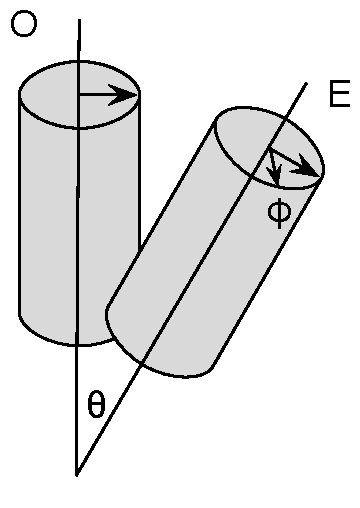
\includegraphics[width=3.5in]{twistSwing}
\caption[The twist-swing decomposition used in orientational
restraints] {The twist-swing decomposition defines relative rotational
  angles using the simplest path to rotate the reference
  configuration.  The reference is rotated by a ``swing'' angle
  $\theta$ in the plane of $\mathbf{O} \times \mathbf{E}$, then
  rotated by a ``twist'' angle $\phi$ around the swing axis.}
\label{fig:twistSwing}
\end{figure}

This illustrates the basic idea of the twist-swing decomposition,
which is a general operation that can be performed on the best-fitting
relative rotation matrix ($\mathsf{A}$) between the instantaneous and
reference structures.  For objects that are not cylindrically
symmetric, there are two swing angles (one in X and one in Y) in
addition to the twist angle.

\begin{code}[caption={[Specifying Restraints for a Molecule] Sample
    keywords defining a molecular restraint and the associated force constants},label={sch:restMol}] 
restraint{
  restraintType = "Molecular";
  molIndex = 0;
  twistSpringConstant = 0.25;
  swingXSpringConstant = 0.02;
  restrainedSwingXAngle = -90.0;
  swingYSpringConstant = 0.02;
  print = "true";
}

useRestraints = "true";
Restraint_file = "prism_ref.inc";
\end{code}

To specify a molecular restraint, it is necessary to give an exact
index of this molecule in the {\tt molIndex} parameter.  In the
example in schem \ref{sch:restMol}, the restrained SwingX angle is -90
degrees offset from the reference structure, so the molecule will be
restrained in a different orientation from the reference geometry.

\begin{longtable}[c]{ABCD}
\caption{Meta-data Keywords: Restraint Parameters}
\\
{\bf keyword} & {\bf units} & {\bf use} & {\bf remarks}  \\ \hline
\endhead
\hline
\endfoot
{\tt restraintType} & string & What kind of restraint is this? &
choose either {\tt Object} or {\tt Molecular} \\
{\tt molIndex} & integer & Which molecule to restrain & \\
{\tt objectSelection} & string & Selection script for Object
restraints & \\
{\tt displacementSpringConstant} &  & & \\
 &  kcal/mol/\AA$^2$ & $k_\mathrm{trans}$ & \\
{\tt twistSpringConstant} & kcal/mol/rad$^2$ & $k_\mathrm{twist}$ & \\
{\tt swingXSpringConstant} & kcal/mol/rad$^2$ & $k_\mathrm{swingX}$ & \\
{\tt swingYSpringConstant} & kcal/mol/rad$^2$ & $k_\mathrm{swingY}$ & \\
{\tt restrainedTwistAngle} & degrees & $\omega_0$ (optional) &
defaults to 0\\
{\tt restrainedSwingXAngle} & degrees & $\theta_0^x$ (optional) & defaults to 0 \\
{\tt restrainedSwingYAngle} & degrees & $\theta_0^y$ (optional) & defaults to 0\\
{\tt print} & logical & whether or not to print restraint value and energy  &
defaults to {\tt true}
\label{table:restraintParams}
\end{longtable}

The various parameters for a {\tt restraint} are shown in table
\ref{table:restraintParams}. Because restraints have a large number of
parameters, these must be enclosed in a {\it separate} {\tt
  restraint\{...\}} block.

\chapter{\label{chapter:perturbations}Perturbations}
OpenMD allows the user to specify two external perturbations that
interact with the electrostatic properties of the atoms.

\section{\label{sec:UniformField}Uniform Fields} 
To apply a uniform
(vector) electric field to the system, the user adds the {\tt
  uniformField} parameter to the MetaData section of the .omd file.

\begin{code}[caption={Specifying a uniform electric field.},label={sch:uniformField}]
   uniformField = (a, b, c);  
\end{code}

The values of $a$, $b$, and $c$ are in units of V~/~\AA.  The
electrostatic potential corresponding to this uniform field is
\begin{equation}
\phi(\mathbf{r})  = - a x - b y - c z
\end{equation}
which grows unbounded and is not periodic.  For these reasons, care
should be taken in using a uniform field with point charges.
The field itself is 
\begin{equation}
\mathbf{E} = \left( \begin{array}{c} a \\ b \\ c \end{array} \right).
\end{equation}
The uniform field applies a force on charged atoms, $ \mathbf{F} = C
\mathbf{E}$.  For dipolar atoms, the uniform field applies both a
potential, $ U = - \mathbf{D} \cdot \mathbf{E}$ and a torque, $
\mathbf{\tau} = \mathbf{D} \times \mathbf{E}$ that depends on the
instantaneous dipole ($\mathbf{D}$) of that atom.

\section{\label{sec:UniformGradient}Uniform Field Gradients} 
To apply a uniform electric field gradient to the system, the user
adds three parameters to the MetaData section

\begin{code}[caption={Specifying a uniform electric field gradient.},label={sch:uniformFieldGradient}]
    uniformGradientStrength = g;
    uniformGradientDirection1 = (a1, a2, a3)
    uniformGradientDirection2 = (b1, b2, b3);
\end{code}

The two direction vectors, $\mathbf{a}$ and $\mathbf{b}$ are unit
vectors, and the value of $g$ is in units of
V~/~\AA\textsuperscript{2}. The electrostatic potential corresponding
to this uniform gradient is
\begin{align}
\phi(\mathbf{r})  = - \frac{g}{2} \Big[&
    \left(a_1 b_1 - \frac{\cos\psi}{3}\right) x^2
    + (a_1 b_2 + a_2 b_1) x y + (a_1 b_3 + a_3 b_1) x z \\
    & + (a_2 b_1 + a_1 b_2) y x 
    + \left(a_2 b_2 - \frac{\cos\psi}{3}\right) y^2
    + (a_2 b_3 + a_3 b_2) y z \\
    & \left. + (a_3 b_1 + a_1 b_3) z x 
    + (a_3 b_2 + a_2 b_3) z y
    + \left(a_3 b_3 - \frac{\cos\psi}{3}\right) z^2 \right]. \\
\end{align}
where $\cos \psi = \mathbf{a} \cdot \mathbf{b}$.  Note that this
potential grows unbounded and is not periodic.  For these reasons,
care should be taken in using a Uniform Gradient with point
charges. The corresponding field for this potential is:
\begin{equation}
\mathbf{E} = \frac{g}{2} \left( \begin{array}{c} 
    2\left(a_1 b_1 - \frac{\cos\psi}{3}\right) x +  (a_1 b_2 + a_2 b_1) y 
    + (a_1 b_3 + a_3 b_1) z  \\
    (a_2 b_1 + a_1 b_2)  x + 2 \left(a_2 b_2 - \frac{\cos\psi}{3}\right) y 
    + (a_2 b_3 + a_3 b_2) z \\
    (a_3 b_1 + a_1 b_3) x +  (a_3 b_2 + a_2 b_3) y 
    + 2 \left(a_3 b_3 - \frac{\cos\psi}{3}\right) z \end{array}
\right).
\end{equation}
The field also grows unbounded and is not periodic.  For these reasons,
care should be taken in using a Uniform Gradient with point dipoles.

The corresponding field gradient,
\begin{equation}
\nabla \mathbf{E} = \frac{g}{2} \left( \begin{array}{ccc}  
    2\left(a_1 b_1 - \frac{\cos\psi}{3}\right)  &  
    (a_1 b_2 + a_2 b_1) & (a_1 b_3 + a_3 b_1) \\
    (a_2 b_1 + a_1 b_2)  & 2 \left(a_2 b_2 - \frac{\cos\psi}{3}\right) & 
    (a_2 b_3 + a_3 b_2) \\
    (a_3 b_1 + a_1 b_3) & (a_3 b_2 + a_2 b_3) & 
    2 \left(a_3 b_3 - \frac{\cos\psi}{3}\right) \end{array} \right)
\end{equation}
is uniform everywhere. The uniform field gradient applies a force on
charged atoms, $\mathbf{F} = C~\mathbf{E}(\mathbf{r})$.  For dipolar
atoms, the gradient applies a potential, $U = -\mathbf{D} \cdot
\mathbf{E}(\mathbf{r})$, force, $\mathbf{F} = \mathbf{D} \cdot
\nabla \mathbf{E}$, and torque, $ \mathbf{\tau} = \mathbf{D} \times
\mathbf{E}(\mathbf{r})$.  For quadrupolar atoms, the uniform field
gradient exerts a potential, $U = - \mathsf{Q}:\nabla \mathbf{E}$, and
a torque $ \mathbf{F} = 2 \mathsf{Q} \times \nabla \mathbf{E}$.

Here, the $:$ indicates a tensor contraction (double dot product) of
two matrices, and the $\times$ for the quadrupole indicates a vector
(cross) product of two matrices, defined as
\begin{equation}
\left[\mathsf{A} \times \mathsf{B}\right]_\alpha = \sum_\beta
\left[\mathsf{A}_{\alpha+1,\beta} \mathsf{B}_{\alpha+2,\beta}
  -\mathsf{A}_{\alpha+2,\beta} \mathsf{B}_{\alpha+1,\beta} 
\right]
\label{eq:matrixCross}
\end{equation}
where $\alpha+1$ and $\alpha+2$ are regarded as cyclic
permuations of the matrix indices.

\section{\label{sec:Light}Light} 
To add a time-dependent oscillating electromagnetic field representing
light, the user may specify a \texttt{light} block in the MetaData
section,

\begin{code}[caption={Specifying a light field using intensity,
wavelength, and propagation direction.},label={sch:light1}]
    light{
      useLight = true;
      intensity = c;
      wavelength = l;
      propagationDirection = (0, 0, 1);
      polarization = "+";
    }
\end{code}

\noindent where the \texttt{propagationDirection} vector is a unit
vector, the \texttt{intensity} is in units of $\mathrm{W~cm^{-2}}$,
and \texttt{wavelength} is in nm. Alternatively, the user
can specify

\begin{code}[caption={Specifying a light field using intensity,
frequency, and propagation direction.},label={sch:light2}]
    light{
      useLight = true;
      intensity = c;
      frequency = w;
      propagationDirection = (0, 0, 1);
      polarization = "+";
    }
\end{code}

\noindent with \texttt{frequency} measured in Hz, or alternatively:

\begin{code}[caption={Specifying a light field using intensity
and wave vector.},label={sch:light3}]
    light{
      useLight = true;
      intensity = c;
      waveVector = (kx, ky, kz);
      polarization = "+";
    }
\end{code}

\noindent with the components of the \texttt{waveVector} specified in $\angstrom^{-1}$.
In all cases, options for \texttt{polarization} include \texttt{"x"},
\texttt{"y"}, \texttt{"+"}, or \texttt{"-"}.  

The field produced by the light block is computed in the reference
frame of the light's direction of propagation,
\begin{equation}
\mathbf{E}_k = \operatorname{Re} \left[ \mathbf{J} \cdot  e^{i \mathbf{k}\cdot \mathbf{r}^\prime -
      \omega t} \right]
  \end{equation}
  where $\mathbf{J}$ is the Jones vector corresponding to the
  polarization of the light, and
  $\mathbf{r}^\prime = \mathsf{A}\cdot \mathbf{r}$ is the position of
  each site in the reference frame of the wave vector, and
  $\mathsf{A}$ is the rotation matrix for the coordinate
  transformation between the lab frame and the propagation
  direction. The electric field is then rotated back into the lab frame,
  \begin{equation}
    \mathbf{E} = \mathsf{A}^{-1} \cdot \mathbf{E}_k,\end{equation}
  and a magnetic
  field is also computed,
  \begin{equation}
    \mathbf{B} = \frac{\mathbf{E} \times
      \hat{\mathbf{k}}}{c}.\end{equation}
  Individual atomic sites with charges and/or dipoles
  interact with both the electric and magnetic fields, although the
  electric field component is typically much larger.

\chapter{\label{section:thermInt}Thermodynamic Integration}

Thermodynamic integration is an established technique that has been
used extensively in the calculation of free energies for condensed
phases of
materials.\cite{Frenkel84,Hermens88,Meijer90,Baez95a,Vlot99}.  This
method uses a sequence of simulations during which the system of
interest is converted into a reference system for which the free
energy is known analytically ($A_0$).  The difference in potential
energy between the reference system and the system of interest
($\Delta V$) is then integrated in order to determine the free energy
difference between the two states:
\begin{equation}
 A = A_0 + \int_0^1 \left\langle \Delta V \right\rangle_\lambda
d\lambda.
\label{eq:thermInt}
\end{equation}
Here, $\lambda$ is the parameter that governs the transformation
between the reference system and the system of interest.  For
crystalline phases, an harmonically-restrained (Einstein) crystal is
chosen as the reference state, while for liquid phases, the ideal gas
is taken as the reference state.  

In an Einstein crystal, the molecules are restrained at their ideal
lattice locations and orientations. Using harmonic restraints, as
applied by B\`{a}ez and Clancy, the total potential for this reference
crystal ($V_\mathrm{EC}$) is the sum of all the harmonic restraints,
\begin{equation}
V_\mathrm{EC} = \sum_{i} \left[ \frac{K_\mathrm{v}}{2} (r_i - r_i^\circ)^2 +
\frac{K_\theta}{2} (\theta_i - \theta_i^\circ)^2 +
\frac{K_\omega}{2}(\omega_i - \omega_i^\circ)^2 \right],
\end{equation}
where $K_\mathrm{v}$, $K_\mathrm{\theta}$, and $K_\mathrm{\omega}$ are
the spring constants restraining translational motion and deflection
of (swing) and rotation around (twist) the principle axis of the
molecule respectively.  The values of $\theta$ range from $0$ to
$\pi$, while $\omega$ ranges from $-\pi$ to $\pi$.

The partition function for a molecular crystal restrained in this
fashion can be evaluated analytically, and the Helmholtz Free Energy
({\it A}) is given by
\begin{eqnarray}
\frac{A}{N} = \frac{E_m}{N}\ -\ kT\ln \left (\frac{kT}{h\nu}\right )^3&-&kT\ln \left
[\pi^\frac{1}{2}\left (\frac{8\pi^2I_\mathrm{A}kT}{h^2}\right
)^\frac{1}{2}\left (\frac{8\pi^2I_\mathrm{B}kT}{h^2}\right
)^\frac{1}{2}\left (\frac{8\pi^2I_\mathrm{C}kT}{h^2}\right
)^\frac{1}{2}\right ] \nonumber \\ &-& kT\ln \left [\frac{kT}{2(\pi
K_\omega K_\theta)^{\frac{1}{2}}}\exp\left
(-\frac{kT}{2K_\theta}\right)\int_0^{\left (\frac{kT}{2K_\theta}\right
)^\frac{1}{2}}\exp(t^2)\mathrm{d}t\right ],
\label{ecFreeEnergy}
\end{eqnarray}
where $2\pi\nu = (K_\mathrm{v}/m)^{1/2}$, and $E_m$ is the minimum
potential energy of the ideal crystal.\cite{Baez95a} 

OpenMD can perform the simulations that aid the user in
constructing the thermodynamic path from the molecular system to one
of the reference systems.  To do this, the user sets the value of
$\lambda$ (between 0 \& 1) in the meta-data file.  If the system of
interest is crystalline, OpenMD must be able to find the  {\it
reference} configuration of the system in a file called {\tt
idealCrystal.in} in the directory from which the simulation was run.
This file is a standard {\tt .dump} file, but all information about
velocities and angular momenta are discarded when the file is read. 

The configuration found in the {\tt idealCrystal.in} file is used for 
the reference positions and molecular orientations of the Einstein
crystal.  To complete the specification of the Einstein crystal, a set
of force constants must also be specified; one for displacments of the
molecular centers of mass, and two for displacements from the ideal
orientations of the molecules.  

\begin{code}[caption={[Specifying Restraints for Thermodynamic
    Integration to an Einstein Crystal]Sample keywords defining restraints
    and their force constants for use in Thermodynamic
    Integration to an Einstein Crystal},label={sch:tiSolid}] 
useThermodynamicIntegration = "true";
thermodynamicIntegrationLambda = 0.0;
thermodynamicIntegrationK = 1.0;

restraint{
 restraintType = "object";
 objectSelection = "select SSD_E";
 displacementSpringConstant = 4.3;
 twistSpringConstant = 750;
 swingXSpringConstant = 700;
 swingYSpringConstant = 700;
 print = "false";
}

useRestraints = "true";
Restraint_file = "idealCrystal.in";
\end{code}

To construct a thermodynamic integration path, the user would run a
sequence of $N$ simulations, each with a different value of $\lambda$
between $0$ and $1$.  When {\tt useThermodynamicIntegration} is set to
{\tt true} in the meta-data file and restraints are present, two
additional energy columns are reported in the {\tt .stat} file for the
simulation.  The first, {\tt vRaw}, is the unperturbed energy for the
configuration, and the second, {\tt vHarm}, is the energy of the
harmonic (Einstein) system in an identical configuration. The total
potential energy of the configuration is a linear combination of {\tt
  vRaw} and {\tt vHarm} weighted by the value of $\lambda$.

From a running average of the difference between {\tt vRaw} and {\tt
vHarm}, the user can obtain the integrand in Eq. (\ref{eq:thermInt})
for fixed value of $\lambda$.  

For {\it liquid} thermodynamic integrations, the reference system is
the ideal gas (with a potential exactly equal to 0), so the {\tt
.stat} file contains only the standard columns. The potential energy
column contains the potential of the {\it unperturbed} system (and not
the $\lambda$-weighted potential.  This allows the user to use the 
potential energy directly as the $\Delta V$ in the integrand of
Eq. (\ref{eq:thermInt}). 

\begin{code}[caption={[Specifying Restraints for Thermodynamic
    Integration to an Ideal Gas]Sample keywords for use in Thermodynamic
    Integration to an Ideal Gas},label={sch:tiLiquid}] 
useThermodynamicIntegration = "true";
thermodynamicIntegrationLambda = 1.0;
thermodynamicIntegrationK = 1.0;
\end{code}

Meta-data parameters concerning thermodynamic integrations are given in
Table~\ref{table:thermIntParams}

\begin{longtable}[c]{ABCD}
\caption{Meta-data Keywords: Thermodynamic Integration Parameters}
\\
{\bf keyword} & {\bf units} & {\bf use} & {\bf remarks}  \\ \hline
\endhead
\hline
\endfoot
{\tt useThermodynamicIntegration} & & &  \\
 & logical & perform thermodynamic integration? & default is {\tt false} \\
{\tt thermodynamicIntegrationLambda} & & & \\
 & double & transformation
parameter & Sets how far along the thermodynamic integration path the
simulation will be. \\
{\tt thermodynamicIntegrationK} & & & \\
 & double & & power of $\lambda$
governing shape of integration pathway \\
\label{table:thermIntParams}
\end{longtable}

\chapter{\label{section:rnemd}Reverse Non-Equilibrium Molecular Dynamics (RNEMD)}

There are many ways to compute transport properties from molecular
dynamics simulations.  Equilibrium Molecular Dynamics (EMD)
simulations can be used by computing relevant time correlation
functions and assuming linear response theory holds.  For some transport properties (notably thermal conductivity), EMD approaches
are subject to noise and poor convergence of the relevant
correlation functions. Traditional Non-equilibrium Molecular Dynamics
(NEMD) methods impose a gradient (e.g. thermal or momentum) on a
simulation.  However, the resulting flux is often difficult to
measure. Furthermore, problems arise for NEMD simulations of
heterogeneous systems, such as phase-phase boundaries or interfaces,
where the type of gradient to enforce at the boundary between
materials is unclear.

{\it Reverse} Non-Equilibrium Molecular Dynamics (RNEMD) methods adopt
a different approach in that an unphysical {\it flux} is imposed
between different regions or ``slabs'' of the simulation box.  The
response of the system is to develop a temperature or momentum {\it
  gradient} between the two regions. Since the amount of the applied
flux is known exactly, and the measurement of gradient is generally
less complicated, imposed-flux methods typically take shorter
simulation times to obtain converged results for transport properties.

\begin{figure}
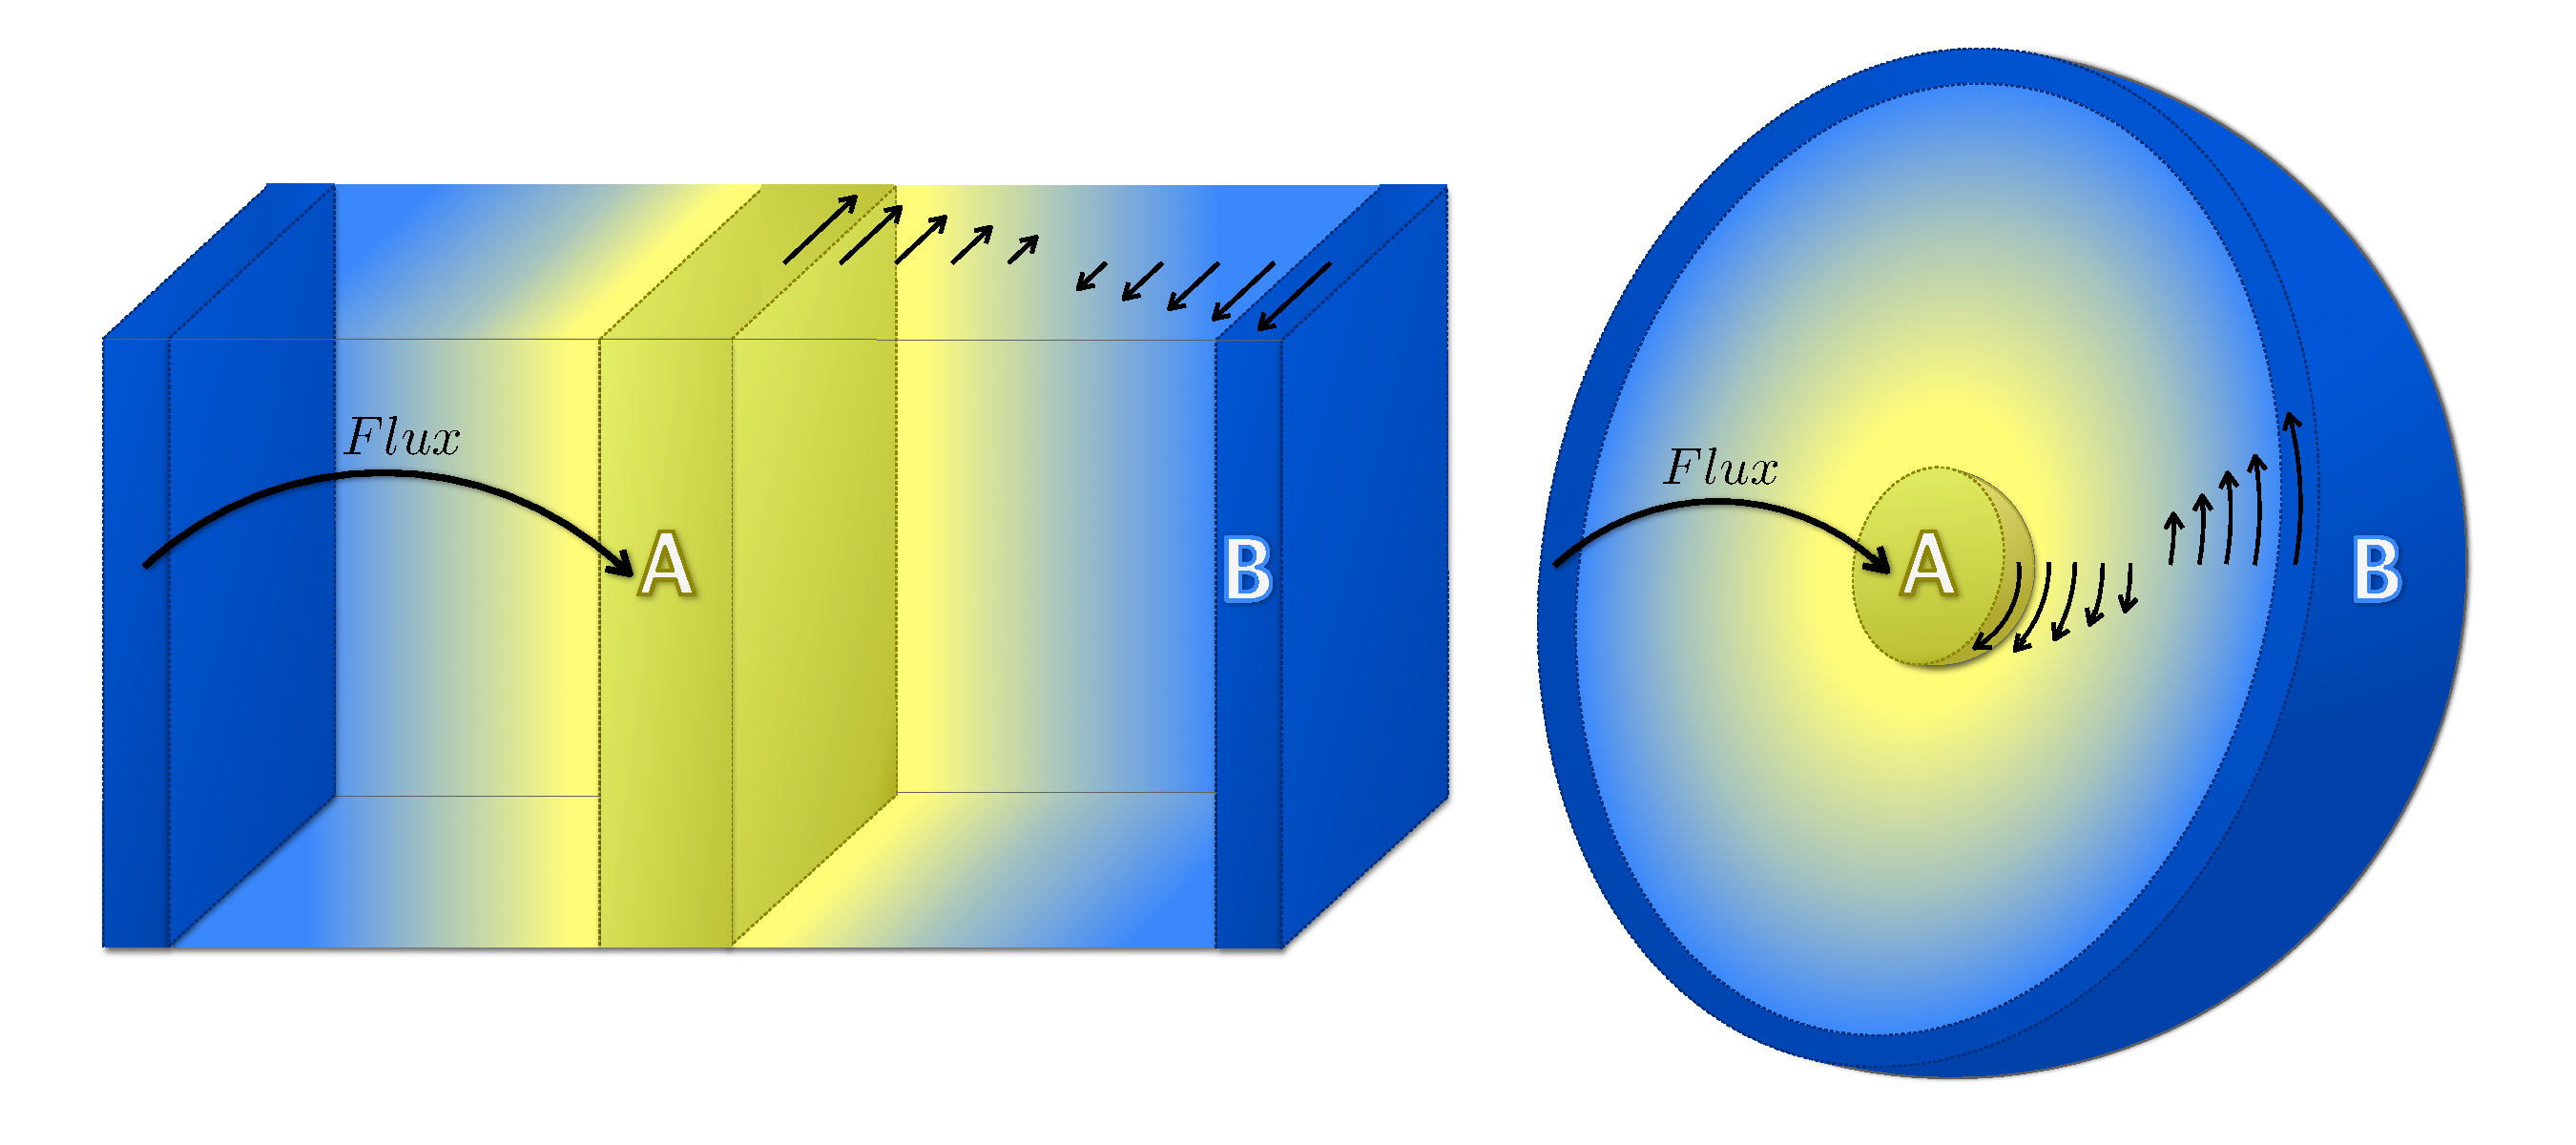
\includegraphics[width=\linewidth]{VSS2}
\caption[Illustration of energy exchange in the VSS RNEMD method]{The
  (VSS) RNEMD approach imposes unphysical transfer of momentum and
  kinetic energy between two regions in a simulation. The system
  responds to this imposed flux by generating velocity and temperature
  gradients. The gradients can then be used to compute transport
  properties (e.g. shear viscosity and thermal conductivity). In
  periodic boundary conditions, linear momentum is exchanged along one
  axis, but for non-periodic (concentric) exchanges, angular momentum
  is exchanged between concentric spheres.}
\label{rnemdDemo}
\end{figure}

\section{\label{section:algo}Algorithms for carrying out RNEMD simulations}
\subsection{\label{subsection:swapping}The swapping algorithm}
The original ``swapping'' approaches by M\"{u}ller-Plathe {\it et
  al.}\cite{ISI:000080382700030,MullerPlathe:1997xw} can be understood
as a sequence of imaginary elastic collisions between particles in
opposite slabs.  In each collision, the entire momentum vectors of
both particles may be exchanged to generate a thermal
flux. Alternatively, a single component of the momentum vectors may be
exchanged to generate a shear flux.  This algorithm turns out to be
quite useful in many simulations. However, the M\"{u}ller-Plathe
swapping approach perturbs the system away from ideal
Maxwell-Boltzmann distributions, and this may leads to undesirable
side-effects when the applied flux becomes large.\cite{Maginn:2010}
This limits the applicability of the swapping algorithm, so in OpenMD,
we have implemented three additional algorithms for RNEMD in addition to the
original swapping approach.

\subsection{\label{subsection:nivs}Non-Isotropic Velocity Scaling (NIVS)}
Instead of having momentum exchange between {\it individual particles}
in each slab, the NIVS algorithm applies velocity scaling to all of
the selected particles in both slabs.\cite{kuang:164101} A combination of linear
momentum, kinetic energy, and flux constraint equations governs the
amount of velocity scaling performed at each step. Interested readers
should consult ref. \citenum{kuang:164101} for further details on the
methodology.

NIVS has been shown to be very effective at producing thermal
gradients and for computing thermal conductivities, particularly for
heterogeneous interfaces.  Although the NIVS algorithm can also be
applied to impose a directional momentum flux, thermal anisotropy was
observed in relatively high flux simulations, and the method is not
suitable for imposing a shear flux or for computing shear viscosities.

\subsection{\label{subsection:vss}Velocity Shearing and Scaling (VSS)}
The third RNEMD algorithm implemented in OpenMD utilizes a series of
simultaneous velocity shearing and scaling exchanges between the two
slabs.\cite{2012MolPh.110..691K}  This method results in a set of simpler equations to satisfy
the conservation constraints while creating a desired flux between the
two slabs.

The VSS approach is versatile in that it may be used to implement both
thermal and shear transport either separately or simultaneously.
Perturbations of velocities away from the ideal Maxwell-Boltzmann
distributions are minimal, and thermal anisotropy is kept to a
minimum.  This ability to generate simultaneous thermal and shear
fluxes has been utilized to map out the shear viscosity of SPC/E water
over a wide range of temperatures (90~K) just with a single simulation.
VSS-RNEMD also allows the directional momentum flux to have
arbitary directions, which could aid in the study of anisotropic solid
surfaces in contact with liquid environments.

\subsection{\label{subsection:spf}Scaled Particle Flux (SPF)}
A final method for carrying out reverse non-equilibrium molecular
dynamics involves migrating particles of a particular type from one
region to another. To create a particle flux, a randomly selected
molecule (of a specific type) is chosen to be migrated from the source
region and into the sink region. This non-physical movement takes
place over a sequence of time steps with a full particle exchange
between source and sink occurring over an exchange period,
$\tau_\mathrm{exch}$. A progress variable, $\lambda$, is introduced to
represent the fraction of a particle which has been transferred
between the two regions at a given time. As $\lambda$ increases from 0
(representing a particle fully present in the source region) to 1
(which represents a particle fully present in the sink region), the
particle coexists in both regions, moving with forces that are
determined from a linear combination of forces with the particle in
both regions, 
\begin{eqnarray}
    U(\mathbf{r}, \lambda) & = \left[1-s(\lambda)\right] ~ U_\mathrm{source}(\mathbf{r}) + s(\lambda)~U_\mathrm{sink}(\mathbf{r}) \\ \label{eq:scalingU}
    \mathbf{F}(\mathbf{r}, \lambda) & = \left[1-s(\lambda)\right] ~ \mathbf{F}_\mathrm{source}(\mathbf{r}) + s(\lambda)~\mathbf{F}_\mathrm{sink}(\mathbf{r})
    \label{eq:scalingF}
\end{eqnarray}
Here, $s(\lambda)$ is a function that moves smoothly from $0
\rightarrow 1$ as $\lambda$ traverses the same
range. $U_\mathrm{source}$ is the potential energy with the particle
fully present in the source region, and $U_\mathrm{sink}$ is the
potential with it fully present in the sink
region. $\mathbf{F}_\mathrm{source}$  and $\mathbf{F}_\mathrm{sink}$
are the corresponding $3N$-vectors of atomic forces. A schematic of
the simulation cell showing the various steps in the method is shown
in Fig. \ref{fig:SPF}.   

\begin{figure}[H]
    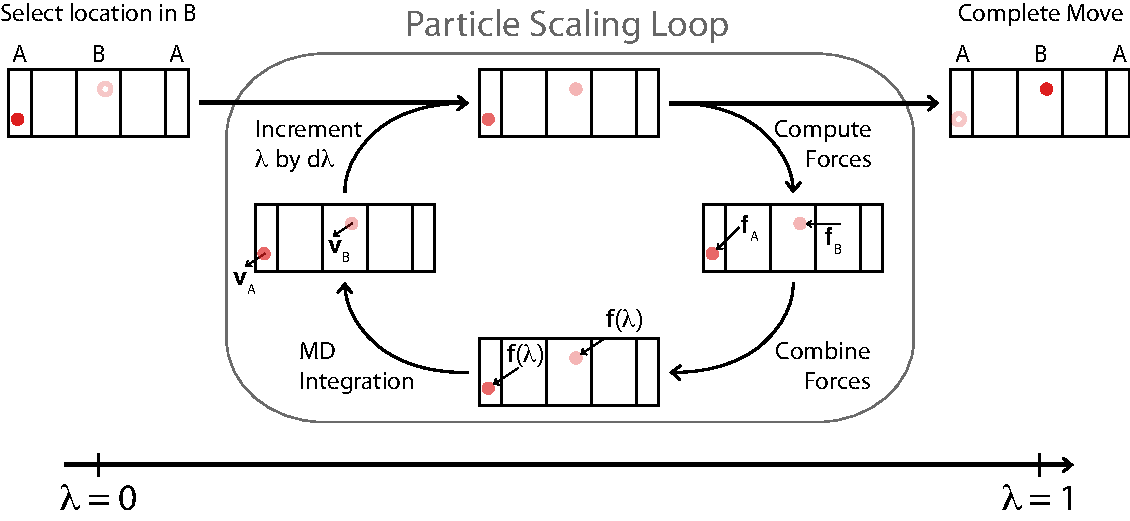
\includegraphics[width=\linewidth]{SPF.pdf}
    \caption[Schematic showing the main steps in the Scaled Particle Flux RNEMD method]{Schematic showing the main steps in the Scaled Particle Flux RNEMD method. A particle in the source bin (A) and a random location in the sink (B) are selected. In the particle scaling loop, all atomic forces using both placements of the particle are computed ($\mathbf{f}_\mathrm{A}$ and $\mathbf{f}_\mathrm{B}$). Forces are combined using the scaling function, $\mathbf{f}(\lambda) = (1-s(\lambda))~\mathbf{f}_\mathrm{A} + s(\lambda)~ \mathbf{f}_\mathrm{B}$, and the system is propagated using standard MD integration with the combined forces. After a successful step, the particle progress variable, $\lambda$ is incremented by $d\lambda$.} 
    \label{fig:SPF} 
\end{figure}

\section{\label{section:nonperiodic}RNEMD in non-periodic geometries}
The original periodic VSS approach uses a series of simultaneous
velocity shearing and scaling exchanges between the two rectangular
slabs in periodic boundary conditions.\cite{2012MolPh.110..691K} This
method imposes constraints which conserve energy and linear momentum 
while simultaneously creating a desired flux between the two
slabs. These constraints ensure that all configurations are sampled
from the same microcanonical (NVE) ensemble.

OpenMD now extends the VSS method for use in {\it non-periodic}
simulations,\cite{Stocker:2014qq} in which the ``slabs'' have been
generalized to two separated regions of space. These regions could be
defined as concentric spheres (as in Figure \ref{rnemdDemo}), or
one of the regions can be defined in terms of a dynamically changing
``hull'' comprising the surface atoms of the cluster. This latter
definition is identical to the hull used in the Langevin Hull
algorithm.\cite{Vardeman2011} For the non-periodic variant of
VSS-RNEMD, the constraints fix both the total energy and total {\it
  angular} momentum of the system while simultaneously imposing a
thermal and {\it angular} momentum flux between the two regions.  This
variant on VSS is particularly useful for simulating heat flow in
nanoparticle / ligand / solvent systems.

For non-periodic simulation cells, it is useful to have exchanges
between concentric regions. To do so, the user must to specify the
radii defining the two exchange regions. There are two parameters for
doing this, {\tt sphereAradius} and {\tt sphereBradius}.  More
complicated regions can also be specified using the selection syntax
described in section \ref{section:syntax}.

\section{\label{section:usingRNEMD}Using OpenMD to perform a RNEMD simulation}
\subsection{\label{section:rnemdParams} What the user needs to specify}

To carry out a RNEMD simulation, a user must specify a number of
parameters in the OpenMD (.omd) file.  Because the RNEMD methods have
a large number of parameters, these must be enclosed in a {\it
  separate} {\tt RNEMD\{...\}} block.  The most important parameters
to specify are the {\tt useRNEMD}, {\tt fluxType} and flux
parameters. Most other parameters (summarized in table
\ref{table:rnemd}) have reasonable default values.  {\tt fluxType}
sets up the kind of exchange that will be carried out between the two
slabs (either Kinetic Energy ({\tt KE}), momentum ({\tt Px, Py, Pz,
  Pvector}) or particle ({\tt Particle}), or some combination of
these).  The flux is specified with the use of four possible
parameters: {\tt kineticFlux} for kinetic energy exchange, as well as
{\tt momentumFlux} or {\tt momentumFluxVector} for simulations with
directional exchange, and {\tt particleFlux} for SPF simulations.  For
concentric exchange, {\tt momentumFlux} and {\tt momentumFluxVector}
are replaced with {\tt angularMomentumFlux} or {\tt
  angularMomentumFluxVector}.

\begin{longtable}[c]{JKLM}
\caption{Meta-data Keywords: Parameters for RNEMD simulations}\\
\multicolumn{4}{c}{The following keywords must be enclosed inside a {\tt RNEMD\{...\}} block.}
\\ \hline
{\bf keyword} & {\bf units} & {\bf use} & {\bf remarks}  \\ \hline
\endhead
\hline
\endfoot
{\tt useRNEMD} & logical & perform RNEMD? & default is ``false'' \\
{\tt objectSelection} & string & see section \ref{section:syntax}
for selection syntax & default is ``select all'' \\
{\tt outputSelection} & string & see section  \ref{section:syntax}
for selection syntax & default is ``select all'' \\
{\tt method} & string & exchange method & one of the following:
{\tt Swap, NIVS, VSS} or {\tt SPF}  (default is {\tt VSS}) \\
{\tt fluxType} & string & defines what is being exchanged between regions & one
of the following: {\tt KE, Px, Py, Pz, Pvector, Lx, Ly, Lz, Lvector, CurrentDensity, Particle, Particle+KE, KE+Px, KE+Py, KE+Pvector, KE+Lx, KE+Ly, KE+Lz, KE+Lvector} \\
{\tt kineticFlux} & kcal mol$^{-1}$ \AA$^{-2}$ fs$^{-1}$ & specify the kinetic energy flux &  \\
{\tt momentumFlux} & amu \AA$^{-1}$ fs$^{-2}$ & specify the momentum flux & \\
{\tt particleFlux} & \AA$^{-2}$ fs$^{-1}$ & specify the particle flux & for SPF method only \\  
{\tt currentDensity} & e \AA$^{-2}$ fs$^{-1}$ & specify the current density & for Charged-SPF method only \\  
{\tt momentumFluxVector} & amu \AA$^{-1}$ fs$^{-2}$ & specify the momentum flux when
{\tt Pvector} is part of the exchange & Vector3d input\\
{\tt angularMomentumFlux} & amu fs$^{-2}$ & specify the angular momentum flux  & for concentric exchange \\
{\tt angularMomentumFluxVector} & & & \\  
  & amu fs$^{-2}$ & specify the angular momentum flux when
{\tt Lvector} is part of the concentric exchange & Vector3d input\\  
{\tt exchangeTime} & fs & how often to perform the exchange & default is 100 fs\\ 
{\tt slabWidth} & $\mbox{\AA}$ & width of the two exchange slabs & default is $\mathsf{H}_{zz} / 10.0$ \\
{\tt slabAcenter} & $\mbox{\AA}$ & center of the end slab & default is 0 \\
{\tt slabBcenter} & $\mbox{\AA}$ & center of the middle slab & default is $\mathsf{H}_{zz} / 2$ \\
{\tt sphereAradius} & $\mbox{\AA}$ & radius of the inner sphere for concentric exchange&  \\
{\tt sphereBradius} & $\mbox{\AA}$ & radius of the outer sphere for concentric exchange&  \\
{\tt selectionA} & string & region A defined with a selection & see section \ref{section:syntax} for selection syntax  \\
{\tt selectionB} & string & region B region defined with a selection & see section \ref{section:syntax} for selection syntax  \\
{\tt dividingArea} & $\mbox{\AA}^2$ & when regions are defined with selections, allows user to specify the dividing area for flux calculations &  \\
{\tt privilegedAxis} & string & in periodic boundaries, perform exchanges along this axis & one
of the following: {\tt x, y, z}, default is {\tt z} \\
{\tt outputFileName} & string & file name for output histograms & default is the same prefix as the
{\tt .omd} file, but with the {\tt .rnemd} extension \\
{\tt outputBins} & int & number of bins in the output histogram & default is 20 \\
{\tt outputBinWidth} & $\mbox{\AA}$ & for concentric exchange, this defines the width of output shells & default is 2 \AA \\
{\tt outputFields} & string & columns to print in the {\tt .rnemd}
file where each column is separated by a pipe ($\mid$) symbol. & Allowed column names are: {\tt z, r, temperature, velocity, angularvelocity, density, activity, electricfield, electrostaticpotential} \\
{\tt spfScalingPower} & int & sets value of $k$ in $s(\lambda) = \lambda^k$
                              (see Eq. \eqref{eq:scalingF}) & default is 3 \\
{\tt spfUniformKineticScaling} &  &  & \\
 & logical & For SPF only, scales velocities in regions A and B identically & default is ``false''
\label{table:rnemd}
\end{longtable}

\subsection{\label{section:rnemdResults} Processing the results} 
OpenMD will generate a {\tt .rnemd} file with the same prefix as the
original {\tt .omd} file.  This file contains a running average of
properties of interest computed within a set of bins that divide the
simulation cell along the $z$-axis (in periodic simulation cells) or
along the radial coordinate, $r$, in concentric exchanges.  The first
column of the {\tt .rnemd} file is the $z$ (or $r$) coordinate of the
center of each bin, while following columns may contain the average
temperature, velocity, density, or activities (concentrations) within
each bin. The output format in the {\tt .rnemd} file can be altered
with the {\tt outputFields}, {\tt outputBins}, {\tt outputBinWidth}, and {\tt
  outputFileName} parameters.  A report at the top of the {\tt .rnemd}
file contains the current exchange totals as well as the average flux
applied during the simulation.  Using the slope of the temperature, velocity, or
concentration gradients obtained from the {\tt .rnemd} file along with the
applied flux, the user can very simply arrive at estimates of thermal
conductivities ($\lambda$),
\begin{equation}
J_z = -\lambda \frac{\partial T}{\partial z},
\end{equation}
and shear viscosities ($\eta$),
\begin{equation}
j_z(p_x) = -\eta \frac{\partial \langle v_x \rangle}{\partial z}.
\end{equation}
or Fick diffusion coefficients ($D$)
\begin{equation}
   x_2 \mathbf{J}_1 = - D \nabla c_1. \label{eq:spfDiffusion}
\end{equation}
Here, the quantities on the left hand side are the actual flux values
(in the header of the {\tt .rnemd} file), while the slopes are
obtained from linear fits to the gradients observed in the {\tt
  .rnemd} file.  Note that $\mathbf{J}_1$ is the externally-applied
particle flux in one component of a binary mixture and $x_2$ is the
mole fraction of the other component.

More complicated simulations (including interfaces) require more
care. Temperature jumps across an interface ($\Delta T$) can be used to
compute the interfacial thermal conductance,
\begin{equation}
  G=\left(\frac{J_z}{\Delta T}\right)
  \label{eq:periodicg}
\end{equation}
For non-periodic (concentric) geometries, it is often better to use
the radial \textit{heat rate}, $q_r$ and to compute interfacial
thermal conductance from the total Kapitza resistance across a
finite-width interfacial region,
\begin{equation}
  \frac{1}{G} = R_\mathrm{total} = \frac{1}{q_r} \sum_i \left(T_{i+i} -
    T_i\right) 4 \pi r_i^2 
\end{equation}
Users interested in interfacial conductance are encouraged to consult
references
\citenum{kuang:AuThl,Stocker:2016kx,Bhattarai:2020lp,Shavalier:2022kn},
and \citenum{Shavalier:2023rm} for other approaches to computing
$G$. Users interested in {\it friction coefficients} at heterogeneous
interfaces may also find references
\citenum{2012MolPh.110..691K,Louden:2017tc}, and
\citenum{Louden:2018le} useful.

\newpage


\subsubsection{\label{section:slipLength}slipLength}
{\tt slipLength} is a built in analysis script which can compute
the slip-length of a solid-liquid interface under shear. The script assumes
the solid is placed in the middle of the box, with equal amounts of
liquid on either side. {\tt slipLength}
reads in the generated {\tt .rnemd} file described above, and returns to
the command line the computed slip-length in Angstroms. There are a few
parameters required to find a good fit of the velocity profile, these are
described in the following table. Also, in order to avoid effects of the
RNEMD exchange bins, the script allows the user to specify the number
of bins to be removed {\tt --toDelete} from the beginning and end of
the simulation box.

\begin{longtable}[c]{|EFG|}
\caption{slipLength Command-line Options}
\\ \hline
{\bf option} & {\bf verbose option} & {\bf behavior} \\ \hline
\endhead
\hline
\endfoot
  -h& {\tt -{}-help}               & Print help and exit\\
  -i& {\tt -{}-input}              & use specified OpenMD (.rnemd) file \\
  -o& {\tt -{}-output}             & specified output file name \\
  -z1& {\tt -{}-lowerGibbsZ}       & the location of the lower Gibbs dividing surface \\
  -z2& {\tt -{}-upperGibbsZ}       & the location of the upper Gibbs dividing surface \\
  -l& {\tt -{}-lowerZVal}          & the initial estimate of the lower interface location (default z1) \\
  -u& {\tt -{}-upperZVal}          & the initial estimate of the upper interface location (default z2) \\
  -w& {\tt -{}-intWidth}           & the width of the interface in Angstroms \\
  -Vs& {\tt -{}-solidVel}          & the initial estimate of the velocity of the solid \\
  -Vl& {\tt -{}-liquidVel}         & the initial estimate of the velocity of the liquid \\
  -m& {\tt -{}-liquidSlope}        & the initial estimate of the slope of the velocity profile in the liquid \\
  -d& {\tt -{}-toDelete}           & the number of data points to be deleted from the beginning and end of the
  velocity profile (default=0) \\
\end{longtable}


\chapter{\label{section:minimizer}Energy Minimization}

Energy minimization is used to identify local configurations that are stable
points on the potential energy surface. There is a vast literature on
energy minimization algorithms have been developed to search for the
global energy minimum as well as to find local structures which are
stable fixed points on the surface.  We have included two simple
minimization algorithms: steepest descent, (SD) and conjugate
gradient (CG) to help users find reasonable local minima from
their initial configurations. Since OpenMD handles atoms and
rigid bodies which have orientational coordinates as well as
translational coordinates, there is some subtlety to the choice of
parameters for minimization algorithms.

Given a coordinate set $x_{k}$ and a search direction $d_{k}$, a line
search algorithm is performed along $d_{k}$ to produce
$x_{k+1}=x_{k}+$ $\lambda _{k}d_{k}$. In the steepest descent (SD) algorithm,
\begin{equation}
d_{k}=-\nabla V(x_{k}).
\end{equation}
The gradient and the direction of next step are always orthogonal.
This may cause oscillatory behavior in narrow valleys.  To overcome
this problem, the Fletcher-Reeves variant~\cite{FletcherReeves} of the
conjugate gradient (CG) algorithm is used to generate $d_{k+1}$
via simple recursion:
\begin{equation}
d_{k+1}  =-\nabla V(x_{k+1})+\gamma_{k}d_{k}
\end{equation}
where
\begin{equation}
\gamma_{k}  =\frac{\nabla V(x_{k+1})^{T}\nabla V(x_{k+1})}{\nabla
V(x_{k})^{T}\nabla V(x_{k})}.
\end{equation}

The Polak-Ribiere variant~\cite{PolakRibiere} of the conjugate
gradient ($\gamma_{k}$) is defined as%
\begin{equation}
\gamma_{k}=\frac{[\nabla V(x_{k+1})-\nabla V(x)]^{T}\nabla V(x_{k+1})}{\nabla
V(x_{k})^{T}\nabla V(x_{k})}%
\end{equation}
It is widely agreed that the Polak-Ribiere variant gives better
convergence than the Fletcher-Reeves variant, so the conjugate
gradient approach implemented in OpenMD is the Polak-Ribiere
variant.

The conjugate gradient method assumes that the conformation is close
enough to a local minimum that the potential energy surface is very
nearly quadratic.  When the initial structure is far from the minimum,
the steepest descent method can be superior to the conjugate gradient
method. Hence, the steepest descent method is often used for the first
10-100 steps of minimization. Another useful feature of minimization
methods in OpenMD is that a modified SHAKE algorithm can
be applied during the minimization to constraint the bond lengths if
this is required by the force field. Meta-data parameters concerning
the minimizer are given in Table~\ref{table:minimizeParams} Because
the minimizer methods have a large number of parameters, these must be
enclosed in a {\it separate} {\tt minimizer\{...\}} block.

\begin{longtable}[c]{ABCD}
\caption{Meta-data Keywords: Parameters for minimization runs}\\
\multicolumn{4}{c}{The following keywords must be enclosed inside a {\tt minimizer\{...\}} block.}
\\ \hline
{\bf keyword} & {\bf units} & {\bf use} & {\bf remarks}  \\ \hline
\endhead
\hline
  \endfoot
  {\tt useMinimizer} & logical &  turns on or off the minimization routines
                                        & default is {\tt false} \\ 
  {\tt method} & string &  selects the minimization method to be used
                                        & either {\tt CG} (conjugate gradient), {\tt SD} (steepest
                                          descent, the default method), or {\tt BFGS} (Broyden-Fletcher-Goldfarb-Shanno) \\ 
  {\tt maxIterations} & steps & Sets the maximum number of iterations
                                for the energy minimization & The default value is 1000\\
  {\tt maxStationaryStateIteration} & &  &  \\
  & steps & sets the maximimum number of steps to take that don't result in a change of configuration  & The default value is 100 \\
  {\tt rootEpsilon} & $\mbox{kcal mol}^{-1}$  & Sets the tolerance
                                                for stopping the minimziation. & The default value is $10^{-5}$\\
  {\tt functionEpsilon} & $\mbox{kcal mol}^{-1}$ &Sets the energy tolerance
                                                for stopping the minimziation. & The default value
                                                                           is  $10^{-5}$\\ 
  {\tt gradientNormEpsilon} & $\mbox{kcal mol}^{-1}\mbox{\AA}^{-1}$  &Sets the gradient tolerance
                                                for stopping the minimziation. & The default 
                                                                                                                   value is $10^{-5}$\\ 
\label{table:minimizeParams}
\end{longtable}

\chapter{\label{section:anal}Analysis of Physical Properties}

OpenMD includes a few utility programs which compute properties
from the dump files that are generated during a molecular dynamics
simulation.  These programs are:

\begin{description}
\item[{\bf Dump2XYZ}] Converts an OpenMD dump file into a file
suitable for viewing in a molecular dynamics viewer like Jmol or VMD
\item[{\bf StaticProps}] Computes static properties like the pair
distribution function, $g(r)$.
\item[{\bf SequentialProps}] Computes a time history of static
  properties from a dump file.
\item[{\bf DynamicProps}] Computes time correlation functions like the
velocity autocorrelation function, $\langle v(t) \cdot v(0)\rangle$,
or the mean square displacement $\langle |r(t) - r(0)|^{2} \rangle$.
\end{description}

These programs often need to operate on a subset of the data contained
within a dump file.  For example, if you want only the {\it oxygen-oxygen}
pair distribution from a water simulation, or if you want to make a
movie including only the water molecules within a 6 angstrom radius of
lipid head groups, you need a way to specify your selection to these
utility programs.  OpenMD has a selection syntax which allows you to
specify the selection in a compact form in order to generate only the
data you want.  For example a common use of the StaticProps command
would be:

{\tt StaticProps -i tp4.dump -{}-gofr  -{}-sele1="select O*"  -{}-sele2="select O*"}

This command computes the oxygen-oxygen pair distribution function,
$g_{OO}(r)$, from a file named {\tt tp4.dump}.  In order to understand
this selection syntax and to make full use of the selection
capabilities of the analysis programs, it is necessary to understand a
few of the core concepts that are used to perform simulations. 

\section{\label{section:concepts}Concepts}

OpenMD manipulates both traditional atoms as well as some objects that
{\it behave like atoms}.  These objects can be rigid collections of
atoms or atoms which have orientational degrees of freedom.  Here is a
diagram of the class heirarchy:

\begin{figure}
\centering
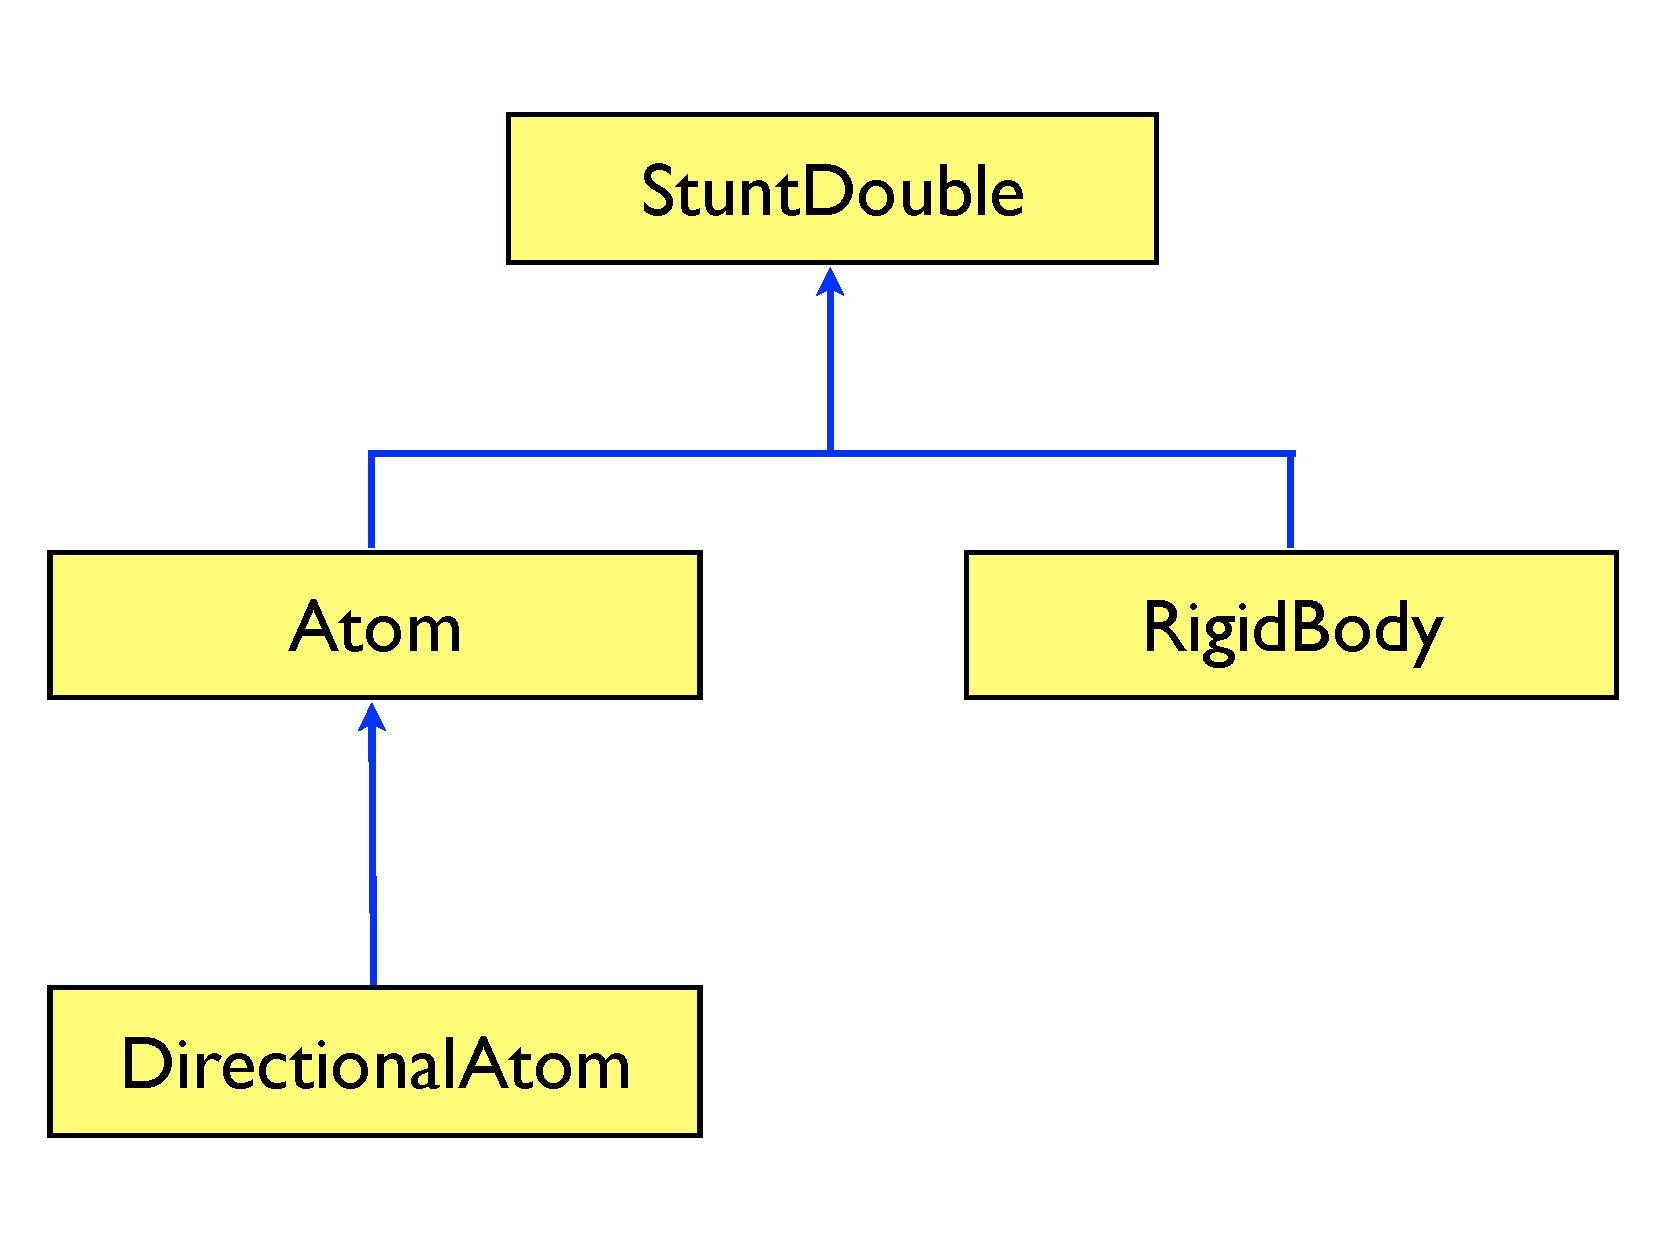
\includegraphics[width=3in]{heirarchy.pdf}
\caption[Class heirarchy for StuntDoubles in OpenMD]{ \\ The
class heirarchy of StuntDoubles in OpenMD. The selection
syntax allows the user to select any of the objects that are descended
from a StuntDouble.}
\label{fig:heirarchy}
\end{figure}

\begin{itemize}
\item A {\bf StuntDouble} is {\it any} object that can be manipulated by the
integrators and minimizers. 
\item An {\bf Atom} is a fundamental point-particle that can be moved around during a simulation.
\item A {\bf DirectionalAtom} is an atom which has {\it orientational} as well as translational degrees of freedom.
\item A {\bf RigidBody} is a collection of {\bf Atom}s or {\bf
DirectionalAtom}s which behaves as a single unit.
\end{itemize} 

Every Molecule, Atom and DirectionalAtom in OpenMD have their
own names which are specified in the {\tt .omd} file. In contrast,
other groupings of atoms are denoted by their membership and index
inside a particular molecule.  For example, RigidBodies are denoted
[MoleculeName]\_RB\_[index] (the contents inside the brackets depend
on the specifics of the simulation). The names of rigid bodies are
generated automatically. For example, the name of the first rigid body
in a DMPC molecule is DMPC\_RB\_0.  Similarly, bonds can be denoted
as: [MoleculeName]\_Bond\_[index], bends as
[MoleculeName]\_Bend\_[index], torsions as
[MoleculeName]\_Torsion\_[index], and inversions as
[MoleculeName]\_Inversion\_[index].  These selection names will select
all of the atoms involved in that group, as well as the grouping
itself.  

\section{\label{section:syntax}Syntax of the Select Command}

The most general form of the select command is: {\tt select {\it expression}}

This expression represents an arbitrary set of StuntDoubles (Atoms or
RigidBodies) in OpenMD. Expressions are composed of either name
expressions, index expressions, predefined sets, user-defined
expressions, comparison operators, within expressions, or logical
combinations of the above expression types. Expressions can be
combined using parentheses and the Boolean operators.

\subsection{\label{section:logical}Logical expressions}

The logical operators allow complex queries to be constructed out of
simpler ones using the standard boolean connectives {\bf and}, {\bf
or}, {\bf not}. Parentheses can be used to alter the precedence of the
operators.

\begin{center}
\begin{tabular}{|ll|}
\hline
{\bf logical operator} & {\bf equivalent operators}  \\  
\hline
and & ``\&'', ``\&\&'' \\
or & ``$|$'', ``$||$'', ``,'' \\
not & ``!''  \\
\hline
\end{tabular}
\end{center}

\subsection{\label{section:name}Name expressions}

\begin{center}
\begin{tabular}{|llp{3in}|}
\hline
{\bf type of expression} & {\bf examples} & {\bf translation of
examples} \\
\hline
expression without ``.'' & {\tt select DMPC} & select all StuntDoubles
belonging to all DMPC molecules \\
 & {\tt select C*} & select all atoms which have atom types beginning with C
\\
 & {\tt select DMPC\_RB\_*} & select all RigidBodies in DMPC molecules (but
only select the rigid bodies, and not the atoms belonging to them). \\
\hline
expression has one ``.'' & {\tt select TIP3P.O\_TIP3P} & select the O\_TIP3P
atoms belonging to TIP3P molecules \\
 & {\tt select DMPC\_RB\_O.PO4} & select the PO4 atoms belonging to
the first 
RigidBody in each DMPC molecule \\
 & {\tt select DMPC.20} & select the twentieth StuntDouble in each DMPC
molecule \\
\hline
expression has two ``.''s & {\tt select DMPC.DMPC\_RB\_?.*} &
select all atoms 
belonging to all rigid bodies within all DMPC molecules \\
\hline
\end{tabular}
\end{center}

\subsection{\label{section:index}Index expressions}

\begin{center}
\begin{tabular}{|lp{4in}|}
\hline
{\bf examples} & {\bf translation of examples} \\
\hline
{\tt select 20} & select all of the StuntDoubles belonging to Molecule 20 \\
{\tt select 20 to 30} & select all of the StuntDoubles belonging to
molecules which have global indices between 20 (inclusive) and 30
(exclusive) \\
\hline
\end{tabular}
\end{center}

\subsection{\label{section:predefined}Predefined sets}

\begin{center}
\begin{tabular}{|ll|}
\hline
{\bf keyword} & {\bf description} \\
\hline
{\tt all} & select all StuntDoubles \\
{\tt none} & select none of the StuntDoubles \\
\hline
\end{tabular}
\end{center}

\subsection{\label{section:userdefined}User-defined expressions}

Users can define arbitrary terms to represent groups of StuntDoubles,
and then use the define terms in select commands. The general form for
the define command is: {\bf define {\it term expression}}

Once defined, the user can specify such terms in boolean expressions

{\tt define SSDWATER SSD or SSD1 or SSDRF}

{\tt select SSDWATER}

\subsection{\label{section:comparison}Comparison expressions}

StuntDoubles can be selected by using comparision operators on their
properties. The general form for the comparison command is: a property
name, followed by a comparision operator and then a number. 

\begin{center}
\begin{tabular}{|l|l|}
\hline
{\bf properties} & {\tt mass, charge, x, y, z, r, wrappedx, wrappedy, wrappedz} \\
{\bf comparison operators} & {\tt <, >, =, >=, <=, !=} \\
\hline
\end{tabular}
\end{center}

For example, the phrase {\tt select mass > 16.0 and charge < -2 }
would select StuntDoubles which have mass greater than 16.0 and charges
less than -2.
 
\subsection{\label{section:within}Within expressions}

The ``within'' keyword allows the user to select all StuntDoubles
within the specified distance (in Angstroms) from a selection,
including the selected atom itself. The general form for within
selection is: {\tt select within(distance, expression)}
 
For example, the phrase {\tt select within(2.5, PO4 or NC4)} would
select all StuntDoubles which are within 2.5 angstroms of PO4 or NC4
atoms.

\section{\label{section:tools}Tools which use the selection command}

\subsection{\label{section:Dump2XYZ}Dump2XYZ}

Dump2XYZ can transform an OpenMD dump file into a xyz file which can
be opened by other molecular dynamics viewers such as Jmol and
VMD. The options available for Dump2XYZ are as follows:


\begin{longtable}[c]{|EFG|}
\caption{Dump2XYZ Command-line Options}
\\ \hline
{\bf option} & {\bf verbose option} & {\bf behavior} \\ \hline
\endhead
\hline
\endfoot
{\tt -h } & {\tt -{}-help} &                        Print help and exit \\
{\tt -V } & {\tt -{}-version} &                     Print version and exit \\
{\tt -i } & {\tt -{}-input=filename}  &             input dump file \\
{\tt -o } & {\tt -{}-output=filename} &             output file name \\
{\tt -n } & {\tt -{}-frame=INT}   &                 print every n frame  (default=`1') \\
{\tt -w } & {\tt -{}-water}       &                 skip the the waters  (default=off) \\
{\tt -m } & {\tt -{}-periodicBox} &                 map to the periodic box  (default=off)\\
{\tt -z } & {\tt -{}-zconstraint}  &                replace the atom types of zconstraint molecules  (default=off) \\
{\tt -r } & {\tt -{}-rigidbody}  &                  add a pseudo COM atom to rigidbody  (default=off) \\
{\tt -t } & {\tt -{}-watertype} &                   replace the atom type of water model (default=on) \\
{\tt -b } & {\tt -{}-basetype}  &                   using base atom type
  (default=off) \\
{\tt -v} & {\tt -{}-velocities}             & Print velocities in xyz file  (default=off)\\
{\tt -f} & {\tt -{}-forces}                 & Print forces xyz file  (default=off)\\
{\tt -u} & {\tt -{}-vectors}                & Print vectors (dipoles, etc) in xyz file  
                                  (default=off)\\
{\tt -c} & {\tt -{}-charges}                & Print charges in xyz file  (default=off)\\
{\tt -e} & {\tt -{}-efield}                 & Print electric field vector in xyz file  
                                  (default=off)\\
     & {\tt -{}-repeatX=INT}  &                 The number of images to repeat in the x direction  (default=`0') \\
     & {\tt -{}-repeatY=INT} &                 The number of images to repeat in the y direction  (default=`0') \\
     &  {\tt -{}-repeatZ=INT}  &                The number of images to repeat in the z direction  (default=`0') \\
{\tt -s } & {\tt -{}-selection=selection script} & By specifying {\tt -{}-selection}=``selection command'' with Dump2XYZ, the user can select an arbitrary set of StuntDoubles to be
converted. \\ 
     & {\tt -{}-originsele} & By specifying {\tt -{}-originsele}=``selection command'' with Dump2XYZ, the user can re-center the origin of the system around a specific StuntDouble \\ 
     & {\tt -{}-refsele} &  In order to rotate the system, {\tt -{}-originsele} and {\tt -{}-refsele} must be given to define the new coordinate set. A StuntDouble which contains a dipole (the direction of the dipole is always (0, 0, 1) in body frame) is specified by {\tt -{}-originsele}. The new x-z plane is defined by the direction of the dipole and the StuntDouble is specified by {\tt -{}-refsele}.
\end{longtable}


\subsection{\label{section:StaticProps}StaticProps}

{\tt StaticProps} can compute properties which are averaged over some
or all of the configurations that are contained within a dump file.
The most common example of a static property that can be computed is
the pair distribution function between atoms of type $A$ and other
atoms of type $B$, $g_{AB}(r)$.  StaticProps can also be used to
compute the density distributions of other molecules in a reference
frame {\it fixed to the body-fixed reference frame} of a selected atom
or rigid body.

There are five seperate radial distribution functions availiable in
OpenMD. Since every radial distrbution function invlove the calculation
between pairs of bodies, {\tt -{}-sele1} and {\tt -{}-sele2} must be specified to tell
StaticProps which bodies to include in the calculation.

\begin{description}
\item[{\tt -{}-gofr}] Computes the pair distribution function,
\begin{equation*}
g_{AB}(r) = \frac{1}{\rho_B}\frac{1}{N_A} \left\langle \sum_{i \in A}
\sum_{j \in B} \delta(r - r_{ij}) \right\rangle
\end{equation*}
\item[{\tt -{}-r\_theta}] Computes the angle-dependent pair distribution
function. The angle is defined by the intermolecular vector $\vec{r}$ and
$z$-axis of DirectionalAtom A,
\begin{equation*}
g_{AB}(r, \cos \theta) = \frac{1}{\rho_B}\frac{1}{N_A} \left\langle \sum_{i \in A}
\sum_{j \in B} \delta(r - r_{ij}) \delta(\cos \theta_{ij} - \cos \theta)\right\rangle
\end{equation*}
\item[{\tt -{}-r\_omega}] Computes the angle-dependent pair distribution
function. The angle is defined by the $z$-axes of the two
DirectionalAtoms A and B. 
\begin{equation*}
g_{AB}(r, \cos \omega) = \frac{1}{\rho_B}\frac{1}{N_A} \left\langle \sum_{i \in A}
\sum_{j \in B} \delta(r - r_{ij}) \delta(\cos \omega_{ij} - \cos \omega)\right\rangle
\end{equation*}
\item[{\tt -{}-theta\_omega}] Computes the pair distribution in the angular
space $\theta, \omega$ defined by the two angles mentioned above.
\begin{equation*}
g_{AB}(\cos\theta, \cos \omega) = \frac{1}{\rho_B}\frac{1}{N_A} \left\langle \sum_{i \in A}
\sum_{j \in B} \delta(\cos \theta_{ij} - \cos \theta)
\delta(\cos \omega_{ij} - \cos \omega)\right\rangle
\end{equation*}
\item[{\tt -{}-gxyz}] Calculates the density distribution of particles of type
B in the body frame of particle A. Therefore, {\tt -{}-originsele} and
{\tt -{}-refsele} must be given to define A's internal coordinate set as
the reference frame for the calculation.
\end{description}

The vectors (and angles) associated with these angular pair
distribution functions are most easily seen in the figure below:

\begin{figure} [H]
\centering
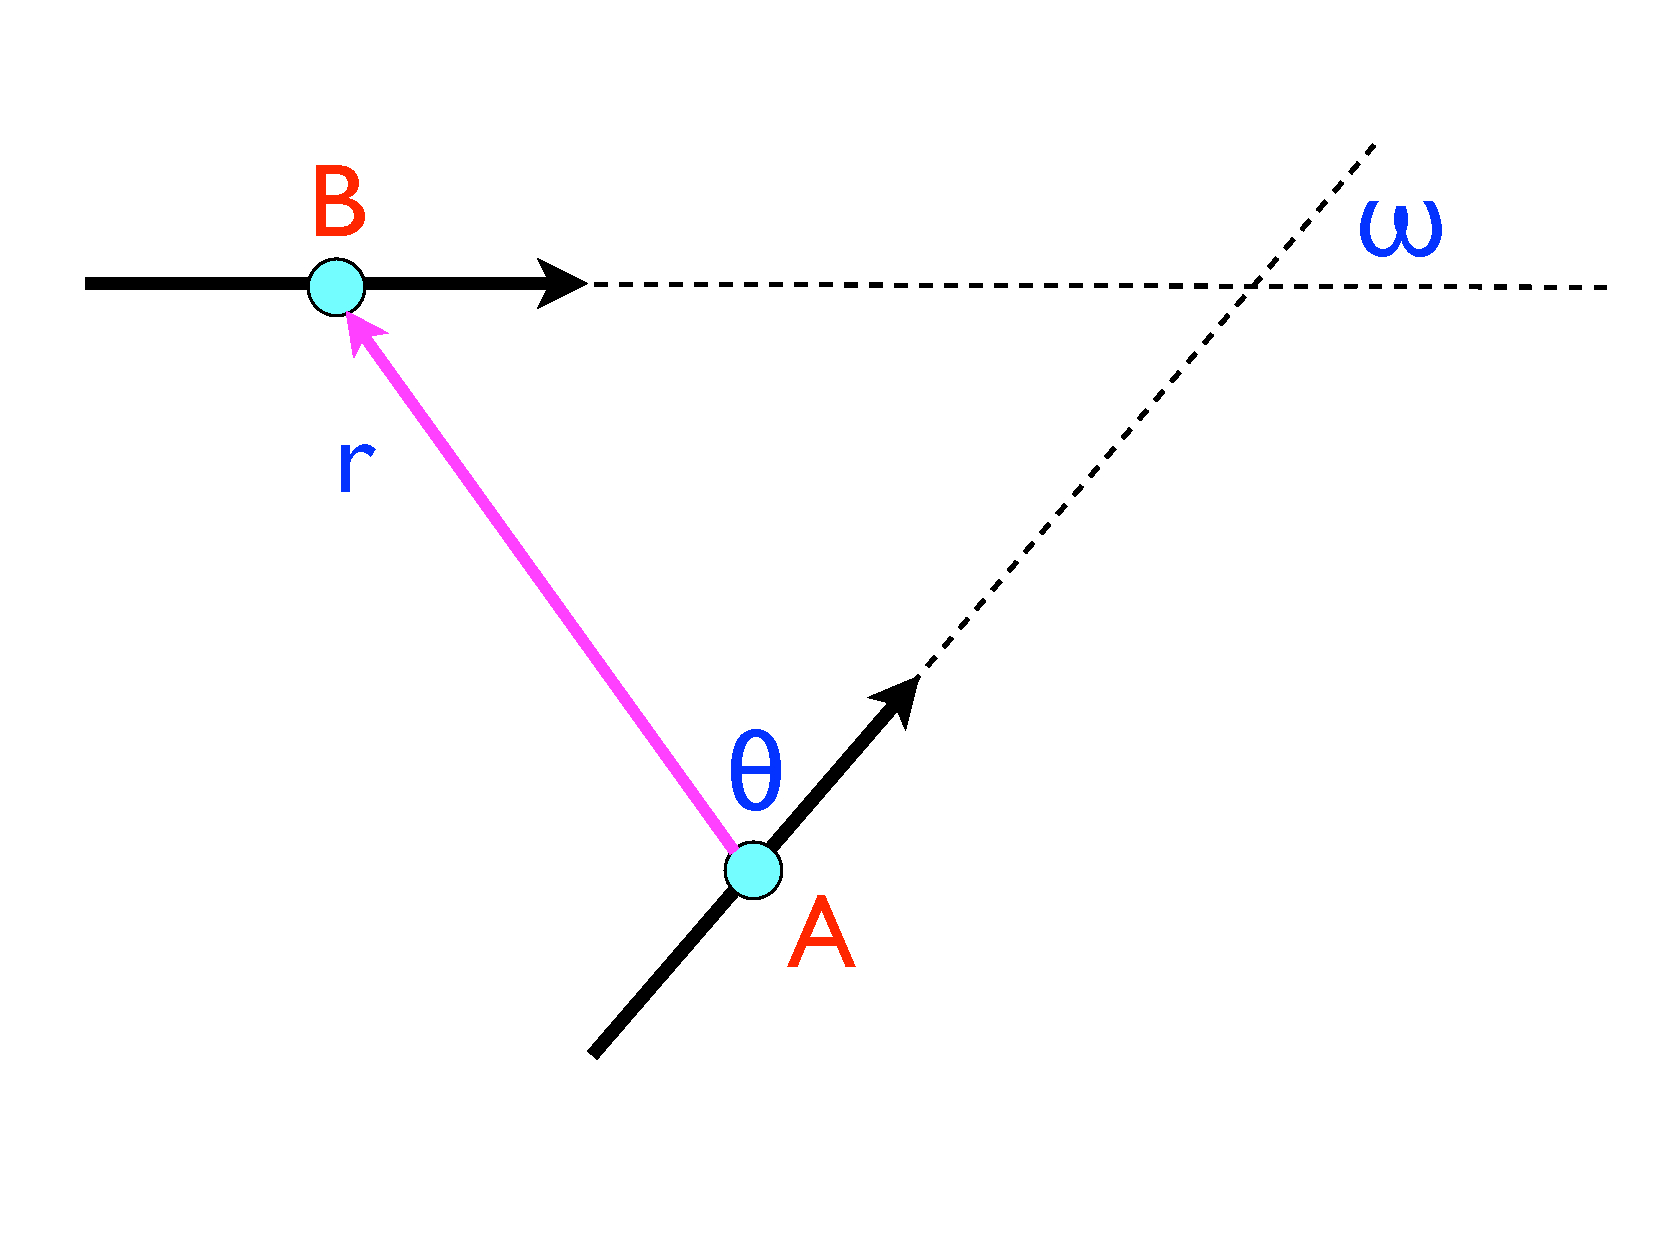
\includegraphics[width=3in]{definition.pdf}
\caption[Definitions of the angles between directional objects]{ \\ Any
two directional objects (DirectionalAtoms and RigidBodies) have a set
of two angles ($\theta$, and $\omega$) between the z-axes of their
body-fixed frames.} 
\label{fig:gofr}
\end{figure}

The options available for {\tt StaticProps} are as follows:
\begin{longtable}[c]{|EFG|}
\caption{StaticProps Command-line Options}
\\ \hline
{\bf option} & {\bf verbose option} & {\bf behavior} \\ \hline
\endhead
\hline
\endfoot
{\tt -h} & {\tt -{}-help}                    &  Print help and exit \\
{\tt -V} & {\tt -{}-version}                 &  Print version and exit \\
{\tt -i} & {\tt -{}-input=filename}          &  input dump file \\
{\tt -o} & {\tt -{}-output=filename}         &  output file name \\
{\tt -n} & {\tt -{}-step=INT}                &  process every n frame
                                          (default=`1') \\
{\tt -b} & {\tt -{}-nbins=INT}               &  number of bins (general
                                          purpose)  (default=`100') \\
{\tt -x} & {\tt -{}-nbins\_x=INT}            & number of bins in x axis  (default=`100')\\
{\tt -y} & {\tt -{}-nbins\_y=INT}            & number of bins in y axis  (default=`100')\\
    & {\tt -{}-nbins\_z=INT}            & number of bins in z axis  (default=`100')\\
{\tt -r} & {\tt -{}-nrbins=INT}              &  number of bins for distance  (default=`100') \\
{\tt -a} & {\tt -{}-nanglebins=INT}          &  number of bins for
                                          cos(angle)  (default= `50')  \\
{\tt -c} & {\tt -{}-rcut=DOUBLE}            & cutoff radius (rcut)\\
    & {\tt -{}-OOcut=DOUBLE}           & Oxygen-Oxygen cutoff radius (angstroms)
                                  (default=`3.5')\\
    & {\tt -{}-thetacut=DOUBLE}        & HOO cutoff angle (degrees)  (default=`30')\\
    & {\tt -{}-OHcut=DOUBLE}        & Oxygen-Hydrogen cutoff radius (angstroms)
                                  (default=`2.45')\\
    & {\tt -{}-dz=DOUBLE}              & slab width (dz)\\

{\tt -l} & {\tt -{}-length=DOUBLE}           &  maximum length (Defaults to 1/2 smallest length of first frame) \\
    & {\tt -{}-zlength=DOUBLE}           &  maximum length (Defaults
                                           to 1/2 smallest length of
                                           first frame) \\
{\tt -z} & {\tt -{}-zoffset=DOUBLE}         & Where to set the zero for the
                                         {\tt slab\_density}
                                  calculation  (default=`0') \\
    & {\tt -{}-sele1=selection script}   & select the first StuntDouble set \\
    & {\tt -{}-sele2=selection script}   & select the second StuntDouble set \\
    & {\tt -{}-sele3=selection script}   & select the third StuntDouble set \\
    & {\tt -{}-refsele=selection script} & select reference (can only
    be used with {\tt -{}-gxyz}) \\
    & {\tt -{}-comsele=selection script}
                               & select stunt doubles for center-of-mass 
                                  reference point\\
    & {\tt -{}-seleoffset=INT}        & global index offset for a second object (used 
                                  to define a vector between sites in molecule)\\
    & {\tt -{}-seleoffset2=INT}        & global index offset for a third object (used 
                                  to define a vector between sites in molecule)\\

    & {\tt -{}-molname=STRING}           & molecule name \\
    & {\tt -{}-begin=INT}                & begin internal index \\
    & {\tt -{}-end=INT}                  & end internal index \\
    & {\tt -{}-radius=DOUBLE}            & nanoparticle radius\\
{\tt -v} & {\tt -{}-voxelSize=DOUBLE}      & voxel size (angstroms) \\
    &  {\tt -{}-gaussWidth=DOUBLE}    &   Gaussian width (angstroms)\\
    & {\tt -{}-privilegedAxis={x,y,z}} & Which axis should
                                                  statistics be
                                                  accumulated along,
                                                  default=z \\
    & {\tt -{}-privilegedAxis2={x,y,z}} & Which axis is special
                                            for spatial analysis,
                                            default=x \\
    & {\tt -{}-momentum={P,J}}         &  Type of momentum
                                          distribution (default=P,
                                           Linear Momentum) \\
      & {\tt -{}-component={x,y,x}}    & Which component of momentum is
                                        sampled for the momemtum
                                         distribution, default=z \\
      & {\tt -{}-dipoleX=DOUBLE}         & X-component of the dipole with respect to body
                                  frame\\
      & {\tt -{}-dipoleY=DOUBLE}         & Y-component of the dipole with respect to body
                                  frame\\
      & {\tt -{}-dipoleZ=DOUBLE}         & Z-component of the dipole with respect to body
                                  frame\\
      & {\tt -{}-v\_radius=DOUBLE}        & VanderWaals radiius for fictious atoms used in
                                  model e.g. M site in TIP4P-FQ water model\\
      & {\tt -{}-gen\_xyz}                & generates xyz file  (default=off)\\
      & {\tt -{}-atom\_name=selection script}
                                & name of atom for with average charge to be
                                  generated\\                                     
\hline
\multicolumn{3}{|l|}{One option from the following group of options is required:} \\
\hline
    & {\tt -{}-bo}          & bond order parameter ({\tt -{}-rcut}
                              must be specified) \\
    & {\tt -{}-ior}        & icosahedral bond order parameter as a function
                                  of radius ({\tt -{}-rcut} must be specified)\\
    & {\tt -{}-for}        & FCC bond order parameter as a function of
                                  radius ({\tt -{}-rcut} must be specified)\\
    & {\tt -{}-bad}         & $N(\theta)$ bond angle density within ({\tt -{}-rcut} must be specified) \\
    & {\tt -{}-count}       & count of molecules matching selection
    criteria (and associated statistics) \\
 {\tt -g} &  {\tt -{}-gofr}                    &  $g(r)$ \\
    &  {\tt -{}-gofz}                    &  $g(z)$ \\
    &  {\tt -{}-r\_theta}                &  $g(r, \cos(\theta))$ \\
    &  {\tt -{}-r\_omega}                &  $g(r, \cos(\omega))$ \\
    &  {\tt -{}-r\_z}                    &  $g(r, z)$ \\
    &  {\tt -{}-theta\_omega}            &  $g(\cos(\theta),
                                           \cos(\omega))$ \\
    &  {\tt -{}-r\_theta\_omega}         &  $g(r, \cos(\theta), \cos(\omega))$ \\
    &  {\tt -{}-gxyz}                    &  $g(x, y, z)$ \\
    &  {\tt -{}-twodgofr}                & 2D $g(r)$ (Slab width {\tt
                                           -{}-dz} must be
                                           specified)\\
    &  {\tt -{}-kirkwood\_buff}          & Kirkwood-Buff integrals ({\tt -{}-sele1} and {\tt -{}-sele2}
                                  must both be specified)\\
{\tt -p} &  {\tt -{}-p2}                      &  $P_2$ order parameter
                                           ({\tt -{}-sele1} must be
                                           specified, {\tt -{}-sele2}
                                           is optional) \\
    &  {\tt -{}-p2r}                   & $P_2$ order parameter using r
                                         as director axis \\
    &  {\tt -{}-rp2}                     &  Ripple order parameter ({\tt -{}-sele1} and {\tt -{}-sele2} must be specified) \\
    &  {\tt -{}-scd}                     &  $S_{CD}$ order parameter(either {\tt -{}-sele1}, {\tt -{}-sele2}, {\tt -{}-sele3} are specified or {\tt -{}-molname}, {\tt -{}-begin}, {\tt -{}-end} are specified) \\
 {\tt -d} &  {\tt -{}-density}                 &  density plot \\
    &  {\tt -{}-slab\_density}           &  slab density, $\rho(z)$ \\
    &  {\tt -{}-pipe\_density}           &  slab density,
                                           $\rho(\mathrm{axis1}, \mathrm{axis2})$\\
    &  {\tt -{}-p\_angle}                & $p(\cos(\theta))$ ($\theta$
    is the angle between molecular axis and radial vector from origin\\
    &  {\tt -{}-hxy}                     & Calculates the undulation  spectrum, $h(x,y)$, of an interface \\
    &  {\tt -{}-rho\_r}                  & $\rho(r)$\\
    &  {\tt -{}-angle\_r}                & $\theta(r)$ (spatially resolves the
    angle between the molecular axis and the radial vector from the
    origin)\\
    &  {\tt -{}-hullvol}                 & hull volume of nanoparticle\\
    &  {\tt -{}-rodlength}               & length of nanorod\\
{\tt -Q} &  {\tt -{}-tet\_param}              & tetrahedrality order parameter ($Q$)\\
    &  {\tt -{}-tet\_param\_z}           & spatially-resolved
                                           tetrahedrality order
                                           parameter $Q(z)$ \\
    & {\tt -{}-tet\_param\_dens} & spatially-resolved tetrahedrality
                                 order parameter Qk(z) \\
    &  {\tt -{}-tet\_param\_xyz}         & volume-resolved tetrahedrality order parameter
                                  $Q(x,y,z)$.  (voxelSize, rcut, and gaussWidth
                                  must be specified)\\
    &  {\tt -{}-rnemdz}                  & slab-resolved RNEMD statistics (temperature, 
                                  density, velocity)\\
    &  {\tt -{}-rnemdr}                  & shell-resolved RNEMD statistics (temperature, 
                                  density, angular velocity) \\
    &  {\tt -{}-rnemdrt}                 & shell and angle-resolved RNEMD statistics
                                  (temperature, density, angular velocity) \\
    &  {\tt -{}-nitrile}                 & electrostatic potential to frequency map based
                                  on the Cho nitrile fits \\
{\tt -m} & {\tt -{}-multipole}               & average multipole moments contained within
                                  cutoff spheres as a function of
                                          radius \\
  & {\tt -{}-cn} & Coordination Number Distribution \\
  & {\tt -{}-scn} & Secondary Coordination Number Distribution \\
    &  {\tt -{}-gcn}                     & Generalized Coordination
                                           Number \\
    &  {\tt -{}-hbond}                   & Hydrogen Bonding statistics using geometric
                                  criteria ({\tt rcut} and {\tt thetacut} must be
                                           specified) \\
    &  {\tt -{}-hbondz}                 & Hydrogen Bonding density binned by z ({\tt rcut} and
                                  {\tt thetacut} must be specified)\\
    &  {\tt -{}-hbondzvol}              & Hydrogen Bonding density binned by z and
                                  normalized by bin volume ({\tt rcut} and {\tt thetacut}
                                  must be specified)\\
    &  {\tt -{}-hbondr}                 & Hydrogen Bonding density binned by r ({\tt rcut} and
                                  {\tt thetacut} must be specified)\\
    &  {\tt -{}-hbondrvol}              & Hydrogen Bonding density binned by r and
                                  normalized by bin volume ({\tt rcut} and {\tt thetacut}
                                  must be specified)\\
    &  {\tt -{}-potDiff}                 & potential energy difference when charge on
                                  selection is set to zero \\
    &  {\tt -{}-tet\_hb}                  & hydrogen bond statistics binned by
                                  tetrahedrality of donor and acceptor
                                  molecules \\
{\tt -k} & {\tt -{}-kirkwood}                & distance-dependent Kirkwood factor \\
    &  {\tt -{}-kirkwoodQ}              &  distance-dependent Kirkwood factor for
                                  quadrupoles \\
 &  {\tt -{}-densityfield}           & density field\\
 &  {\tt -{}-velocityfield}          & velocity field\\
&  {\tt -{}-velocityZ}               & two-dimensional velocity map \\
{\tt -D} &  {\tt -{}-eam\_density}         & EAM density profile \\
{\tt -q} &  {\tt -{}-net\_charge}          & charge profile \\
{\tt -J} &  {\tt -{}-current\_density}    & current density \\
 &  {\tt -{}-chargez}                & computes the charge distribution along selected
                                  axis and selected atom\\
 &  {\tt -{}-charger}                & computes the charge density as a function of
                                  the radius and selected atom\\
 &  {\tt -{}-massdensityz}           & computes the mass density of the selection
                                  along selected axis\\
 &  {\tt -{}-massdensityr}           & computes the mass density of the selection as a
                                  function of the radius from the center of
                                  mass\\
 &  {\tt -{}-numberz}                & computes the number density along selected axis
                                  and selected molcule\\
 &  {\tt -{}-numberr}                & computes the number density as a function of
                                  the radius and selected molecule\\
 &  {\tt -{}-charge\_density\_z}      &  computes the continuous charge distribution
                                  along selected axis and selected atom\\
 &  {\tt -{}-countz}                 & computes the number of selected atoms along selected axis\\
{\tt -M} &  {\tt -{}-momentum\_distribution} &  momentum distribution \\
{\tt -S} &  {\tt -{}-dipole\_orientation}     & spatially-resolved dipole order parameter $S(z)$,
                                  $S = (3 \cos^2\theta - 1)/2$ \\
 &  {\tt -{}-order\_prob}            &  probability of order parameter for given selection
\end{longtable}

\subsection{\label{section:SequentialProps}SequentialProps}

Occasionally, it may be useful to compute a time history of static
properties as a simulation progresses.  The utility {\tt
  SequentialProps} computes these time histories from configurations
stored in a dump file.  Currently, only a few static properties are
available in SequentialProps, but these include contact angles, and
centers of mass.  

For contact angles of droplets on surfaces, two methods are available:
In the first method, the droplet is assumed to form a spherical cap,
and the contact angle is estimated from the $z$-axis location of the
droplet's center of mass ($z_\mathrm{cm}$).  This procedure was first
described by Hautman and Klein.\cite{Hautman91} For each stored
configuration, the contact angle, $\theta$, is found by inverting the
expression for the location of the droplet center of mass,
\begin{equation}\label{contact_1}
\langle z_\mathrm{cm}\rangle = 2^{-4/3}R_{0}\bigg(\frac{1-cos\theta}{2+cos\theta}\bigg)^{1/3}\frac{3+cos\theta}{2+cos\theta} ,
\end{equation}
where $R_{0}$ is the radius of the free droplet before it contacts the
surface. 

A second method for obtaining the contact angle was described by
Ruijter, Blake, and Coninck~\cite{Ruijter99}.  This method uses a
cylindrical averaging of the droplet's density profile.  A threshold
density is used to estimate the location of the edge of the droplet.
The $r$ and $z$-dependence of the droplet's edge is then fit to a
circle, and the contact angle is computed from the intersection of the
fit circle with the $z$-axis location of the solid surface.  For each
stored configuration, the density profile in a set of annular shells
is computed.  The height of the solid surface ($z_\mathrm{suface}$)
along with the best fitting origin ($z_\mathrm{droplet}$) and radius
($r_\mathrm{droplet}$) of the droplet can then be used to compute the
contact angle,
\begin{equation}
\theta =  90 + \frac{180}{\pi} \sin^{-1}\left(\frac{z_\mathrm{droplet} -
  z_\mathrm{surface}}{r_\mathrm{droplet}} \right).
\end{equation}

In studying surfaces, Calle-Vallejo {\it et al.}  observed that
including the first and second nearest neighbor counts allowed for a
more complete description of an atom's local environment and its
catalytic activity.\cite{Calle-Vallejo:2015qq} They introduced the
\textit{generalized coordination number} (GCN), to describe this
quantity,
\begin{equation}
  \overline{CN}(i) = \sum_{j=1}^{n_i}\frac{cn(j)}{cn_{\textrm{max}}}
  \label{eq:gcn}
\end{equation}
The GCN is an extension of nearest-neighbor analysis where the GCN of
atom $i$, $\overline{CN}(i)$, is calculated from the average of the
coordination numbers, $cn(j)$, of atom $i$'s nearest neighbors ($j$).

The options available for SequentialProps are as follows:
\begin{longtable}[c]{|EFG|}
\caption{SequentialProps Command-line Options}
\\ \hline
{\bf option} & {\bf verbose option} & {\bf behavior} \\ \hline
\endhead
\hline
\endfoot
{\tt -h} & {\tt -{}-help}                   & Print help and exit \\
{\tt -V} & {\tt -{}-version}                & Print version and exit \\
{\tt -i} & {\tt -{}-input=filename}         & input dump file (mandatory) \\
{\tt -o} & {\tt -{}-output=filename}        & output file name \\
    & {\tt -{}-sele1=selection script} & select first stuntdouble set \\
    & {\tt -{}-sele2=selection script} & select second stuntdouble set (if sele2 is not
                                  set, use script from sele1) \\
{\tt -b} & {\tt -{}-nbins=INT}              & number of bins (general purpose)
                                  (default=`100') \\
    & {\tt -{}-nbins\_z=INT}            & number of bins in z axis  (default=`100') \\
{\tt -x} & {\tt -{}-centroidX=DOUBLE}       & Location of droplet centroid in x \\
{\tt -y} & {\tt -{}-centroidY=DOUBLE}       & Location of droplet centroid in y \\
{\tt -z} & {\tt -{}-referenceZ=DOUBLE}      & Reference z-height of solid surface \\
{\tt -r} & {\tt -{}-dropletR=DOUBLE}        & Droplet radius in angstroms \\
    & {\tt -{}-threshDens=DOUBLE}      & Threshold Density in g/cm$^3$ \\
    & {\tt -{}-bufferLength=DOUBLE}    & Buffer length in angstroms \\
    & {\tt -{}-rcut=DOUBLE}            & cutoff radius (rcut) \\
\hline
\multicolumn{3}{|l|}{One option from the following group of options is required:} \\
\hline
{\tt -c} & {\tt -{}-com}                   &  selection center of mass \\
    & {\tt -{}-ca1}                   &  contact angle of selection (using center of
                                  mass)\\
    & {\tt -{}-ca2}                   &  contact angle of selection (using density
                                  profile)\\
    & {\tt -{}-gcn}                   &  Generalized Coordinate
                                        Number\\
 {\tt -t} & {\tt -{}-testequi}     & Temperature using all componets of linear and
                                  angular momentum
\end{longtable}

\subsection{\label{section:DynamicProps}DynamicProps}

{\tt DynamicProps} computes time correlation functions from the
configurations stored in a dump file.  Typical examples of time
correlation functions are the mean square displacement and the
velocity autocorrelation functions.   Once again, the selection syntax
can be used to specify the StuntDoubles that will be used for the
calculation.  A general time correlation function can be thought of
as:
\begin{equation}
C_{AB}(t) = \langle \vec{u}_A(t) \cdot \vec{v}_B(0) \rangle
\end{equation}
where $\vec{u}_A(t)$ is a vector property associated with an atom of
type $A$ at time $t$, and $\vec{v}_B(t^{\prime})$ is a different
vector property associated with an atom of type $B$ at a different
time $t^{\prime}$.  In most autocorrelation functions, the vector
properties ($\vec{v}$ and $\vec{u}$) and the types of atoms ($A$ and
$B$) are identical, and some of the calculations built in to {\tt
  DynamicProps} make these assumptions. It is possible, however, to
make simple modifications to the {\tt DynamicProps} code to allow the
use of {\it cross} time correlation functions (i.e. with different
vectors).  The ability to use two selection scripts to select
different types of atoms is already present in the code.

The options available for DynamicProps are as follows:
\begin{longtable}[c]{|EFG|}
\caption{DynamicProps Command-line Options}
\\ \hline
{\bf option} & {\bf verbose option} & {\bf behavior} \\ \hline
\endhead
\hline
\endfoot
{\tt -h} & {\tt -{}-help}                   & Print help and exit \\
{\tt -V} & {\tt -{}-version}                & Print version and exit \\
{\tt -i} & {\tt -{}-input=filename}         & input dump file \\
{\tt -o} & {\tt -{}-output=filename}        & output file name \\
    & {\tt -{}-sele1=selection script} & select first StuntDouble set \\
    & {\tt -{}-sele2=selection script} & select second StuntDouble set
                                         (if sele2 is not set, use
                                         script from sele1) \\
    & {\tt -{}-sele3=selection script} & select third stuntdouble set\\
    & {\tt -{}-order=INT}              & Lengendre Polynomial Order\\
{\tt -z} & {\tt -{}-nzbins=INT}             & Number of $z$ bins (default=`100`)\\
{\tt -c} & {\tt -{}-rcut=DOUBLE}            & cutoff radius (angstroms)\\
    & {\tt -{}-OOcut=DOUBLE}           & Oxygen-Oxygen cutoff radius (angstroms)
                                  (default=`3.5')\\
    & {\tt -{}-thetacut=DOUBLE}        & HOO cutoff angle (degrees)  (default=`30')\\
    & {\tt -{}-OHcut=DOUBLE}           & Oxygen-Hydrogen cutoff radius (angstroms)
                                  (default=`2.45')\\
    & {\tt -{}-privilegedAxis={x,y,z}} & Which axis should
                                                  statistics be
                                                  accumulated along,
                                                  default=z \\
    & {\tt -{}-length=DOUBLE}          & maximum length  (default=`100')\\
    & {\tt -{}-dipoleX=DOUBLE}         & X-component of the dipole with respect to body
                                  frame  (default=`0.0')\\
    & {\tt -{}-dipoleY=DOUBLE}         & Y-component of the dipole with respect to body
                                  frame  (default=`0.0')\\
    & {\tt -{}-dipoleZ=DOUBLE}         & Z-component of the dipole with respect to body
                                  frame  (default=`-1.0')\\
\hline
\multicolumn{3}{|l|}{One option from the following group of options is required:} \\
\hline
{\tt -s} & {\tt -{}-selecorr}        & selection correlation function \\
{\tt -r} & {\tt -{}-rcorr}           & compute mean squared displacement \\
    & {\tt -{}-rcorrZ}               & mean squared displacement binned by Z\\
{\tt -v} & {\tt -{}-vcorr}           & velocity autocorrelation function \\
    & {\tt -{}-vcorrZ}               & autocorrelation function of velocity projected along privileged axis\\
    & {\tt -{}-vcorrR}               & radially-projected velocity autocorrelation function\\
    & {\tt -{}-vaOutProdcorr}        & Velocity outer product autocorrelation function\\
    & {\tt -{}-waOutProdcorr}        & Angular Velocity outer product autocorrelation function\\
    & {\tt -{}-vwOutProdcorr}        & Velocity - Angular Velocity outer product cross-correlation function\\
    & {\tt -{}-wvOutProdcorr}        & Angular Velocity - Velocity outer product cross-correlation function\\
{\tt -w} & {\tt -{}-wcorr}           & fluctuating charge velocity autocorrelation function \\
{\tt -d} & {\tt -{}-dcorr}           & dipole correlation function \\
{\tt -l} & {\tt -{}-lcorr}           & Lengendre correlation function \\
    & {\tt -{}-lcorrZ}               & Lengendre correlation function binned by $z$ \\
    & {\tt -{}-cohZ}                 & Lengendre correlation function for OH bond vectors binned by $z$\\
{\tt -M} & {\tt -{}-sdcorr}          & System dipole correlation function\\
    & {\tt -{}-r\_rcorr}             & Radial mean squared displacement\\
    & {\tt -{}-thetacorr}            & Angular mean squared displacement\\
    & {\tt -{}-drcorr}               & Directional mean squared displacement for particles with unit vectors\\
    & {\tt -{}-stresscorr}           & Stress tensor correlation function\\
{\tt -b} & {\tt -{}-bondcorr}        & Bond extension correlation function\\
{\tt -f} & {\tt -{}-freqfluccorr}    & Frequency Fluctuation correlation function\\
{\tt -j} & {\tt -{}-jumptime}        & Hydrogen bond jump time correlation function \\
    & {\tt -{}-jumptimeZ}            & Hydrogen bond jump time correlation function binned by Z \\
    & {\tt -{}-jumptimeR}            & Hydrogen bond jump time correlation function binned by R around a third selection \\
    & {\tt -{}-persistence}          & Hydrogen bond persistence correlation function\\
    & {\tt -{}-pjcorr}               & Momentum - Angular Momentum cross correlation function \\
    & {\tt -{}-ftcorr}               & Force - Torque cross correlation function \\
    & {\tt -{}-facorr}               & Force autocorrelation function \\
    & {\tt -{}-tfcorr}               & Torque - Force cross correlation function \\
    & {\tt -{}-tacorr}               & Torque autocorrelation function \\
    & {\tt -{}-disp}                 & Displacement correlation function \\
    & {\tt -{}-dispZ}                & Displacement correlation function binned by Z \\
    & {\tt -{}-current}              & Current density auto correlation function\\
    & {\tt -{}-onsager}              & Onsager coefficient correlation functions\\
    & {\tt -{}-ddisp}                & Collective Dipole displacement function (Helfand moment of Current Density)\\
    & {\tt -{}-rotAngleDisp}         & Displacement correlation function for rotation angles
\end{longtable}


\section{\label{section:utilities}Utilities to aide in analysis}

\subsection{\label{section:omdShrink}omdShrink}
{\tt omdShrink} is a utility script which takes {\tt OpenMD} {\tt .dump}
files as input and generates an output {\tt .dump} file with fewer frames
than in the original {\tt .dump} file. The user passes {\tt omdShrink}
and integer {\tt -s} and the input {\tt .dump} file is split every {\tt -s} 
frames.

\begin{longtable}[c]{|EFG|}
\caption{omdShrink Command-line Options}
\\ \hline
{\bf option} & {\bf verbose option} & {\bf behavior} \\ \hline
\endhead
\hline
\endfoot
{\tt -h} & {\tt -{}-help}        & Print help and exit\\
{\tt -m} & {\tt -{}-meta-data}   & use specified OpenMD (.dump) file \\
{\tt -o} & {\tt -{}-output-file} & specified output file name \\
{\tt -s} & {\tt -{}-split-frame} & split the (.dump) file every s frames \\
\end{longtable}

\subsection{\label{section:omdSplit}omdSplit}
{\tt omdSplit} is a utility script which takes {\tt OpenMD} {\tt .dump}
files and splits them into {\tt -s} separate files.

\begin{longtable}[c]{|EFG|}
\caption{omdSplit Command-line Options}
\\ \hline
{\bf option} & {\bf verbose option} & {\bf behavior} \\ \hline
\endhead
\hline
\endfoot
{\tt -h} & {\tt -{}-help}        & Print help and exit\\
{\tt -m} & {\tt -{}-meta-data}   & use specified OpenMD (.dump) file \\
{\tt -s} & {\tt -{}-split-frame} & split every s frames \\
\end{longtable}



\subsection{\label{section:hbtetAnalyzer}hbtetAnalyzer}
{\tt hbtetAnalyzer} is a utility script which analyzes hydrogen-bond
by tetrahedrality matrices computed via the {\tt StaticProps} module
{\tt --tet\_hb}. This script computes integrals of user defined
regions in the {\tt .hbq} file, and reports the individual sums for
each of the symmetric regions of the matrix as well as the number of
hydrogen-bonds per square Angstrom between the two specified {\tt -qS}
and {\tt -qL}.

\begin{longtable}[c]{|EFG|}
\caption{hbtetAnalyzer Command-line Options}
\\ \hline
{\bf option} & {\bf verbose option} & {\bf behavior} \\ \hline
\endhead
\hline
\endfoot
{\tt -h}  & {\tt -{}-help}        & Print help and exit\\
{\tt -i}  & {\tt -{}-hbq-file}    & use specified OpenMD (.hbq) file \\
{\tt -o}  & {\tt -{}-hbqPAS-file} & use specified output (.hbqPSA) file \\
{\tt -qS} & {\tt -{}-q(liquid)}   & the tetrahedral order parameter value at the solid surface \\
{\tt -qL} & {\tt -{}-q(solid)}    & the tetrahedral order parameter value at the liquid surface \\
{\tt -x}  & {\tt -{}-boxl(x)}     & the x-dimension of the simulation box (Angstroms) \\
{\tt -y}  & {\tt -{}-boxl(y)}     & the y-dimension of the simulation box (Angstroms) \\
{\tt -z}  & {\tt -{}-boxl(z)}     & the z-dimension of the simulation box (Angstroms) \\
{\tt -t}  & {\tt -{}-nSnapshots}  & the number of snapshots used to accumulate the (.hbq) file \\
\end{longtable}

\section{stat2- utility scripts}
{\tt OpenMD} contains a set of utility scripts which take ({\tt
  .stat}) files as inputs and compute properties about the
system. 

\subsection{\label{section:stat2dielectric}stat2dielectric}
The {\tt stat2dielectric} utility script computes the static
dielectric constant of the system from a corresponding ({\tt .stat})
file where the ({\tt .omd}) file has had the {\tt SYSTEM\_DIPOLE} added
to the {\tt statFileFormat} line. A brief description of the
calculations performed by the script is given below, and further
information is available from the help prompt ({\tt -h}) from
{\tt stat2dielectric}. 

This script assumes the fluctuation formula appropriate for conducting
boundaries:
\begin{equation}
\epsilon_\mathrm{A} = 1 + \frac{\left\langle M^{2}\right\rangle -
  \left\langle M \right\rangle^{2}}{3k_{B}\left\langle T\right\rangle
  \left\langle V \right\rangle \epsilon_{0}}
\end{equation}
where $\epsilon_\mathrm{A}$ is the dielectric constant of the system,
$M$ is the total dipole moment of the simulation box,$\langle V \rangle$ is the
average volume of the box, $\langle T \rangle$ is the average temperature of the
box, $\epsilon_{0}$ is the permittivity of a vacuum, and $k_{B}$ is
Boltzmann's constant. 

This script will also optionally apply a correction factor as follow:
\begin{equation}
\epsilon = \frac{((Q + 2) (\epsilon_{A} - 1) + 3)}{((Q - 2) (\epsilon_{A} - 1) + 3)}
\end{equation}
where $Q$ depends on the method used to compute the electrostatic
interaction.

\begin{longtable}[c]{|EFG|}
\caption{stat2dielectric Command-line Options}
\\ \hline
{\bf option} & {\bf verbose option} & {\bf behavior} \\ \hline
\endhead
\hline
\endfoot
{\tt -h} & {\tt -{}-help}        & Print help and exit\\
{\tt -f} & {\tt -{}-stat-file}   & use specified OpenMD (.stat) file \\
{\tt -o} & {\tt -{}-output-file} & use specified output (.dielectric) file\\
{\tt -q} & {\tt -{}-Q-value}     & use the specified Q value to correct the dielectric \\
\end{longtable}

\subsection{\label{section:stat2tension}stat2tension}
The {\tt stat2tension} utility script computes the surface tension of
the system from a corresponding ({\tt .stat}) file where the ({\tt
  .omd}) file has had the {\tt PRESSURE\_TENSOR} added to the {\tt
  statFileFormat} line. A brief description of the calculations
performed by the script is given below, and further information is
available from the help prompt ({\tt -h}) from {\tt stat2tension}.

This script assumes that the interface is normal to the $z$-axis,
i.e., $P_{n} = P_{zz}$, and that the tangential contributions are
averaged over the remaining axes, 
\begin{equation}
P_{t}(z) = ( P_{xx} + P_{yy}) / 2
\end{equation}
The surface tension is defined using the normal and tangential
components of the pressure,
\begin{equation}
\gamma = \int_{-\infty}^{\infty} \left(P_{n} - P_{t}(z)\right) dz.
\end{equation} 

The tangential pressure is different from the normal pressure only in
the vicinity of the interfaces, so the net surface tension for the
system can be simplified:
\begin{equation}
\gamma = L_{z} \left( P_{n} - \langle P_{t} \rangle \right)
\end{equation}
where $\langle P_{t} \rangle$ is the statistical average of the
tangential pressure.

In practice, many surface tension simulations comprise two regions,
with one material in each region.  Periodic boundary conditions then
require two interfaces, so
\begin{equation}
  \gamma = L_{z} \left(P_{n} - \langle P_{t} \rangle \right)
\end{equation}

\begin{longtable}[c]{|EFG|}
\caption{stat2tension Command-line Options}
\\ \hline
{\bf option} & {\bf verbose option} & {\bf behavior} \\ \hline
\endhead
\hline
\endfoot
{\tt -h} & {\tt -{}-help}        & Print help and exit\\
{\tt -s} & {\tt -{}-stat-file}   & use specified OpenMD (.stat) file \\
{\tt -o} & {\tt -{}-output-file} & use specified output (.tension) file\\
{\tt -z} & {\tt -{}-box-length}  & dimension of the system box in the normal (z) direction \\
\end{longtable}

%\subsection{\label{section:stat2thcond}stat2thcond}
% Code currently broken.

\subsection{\label{section:stat2visco}stat2visco}
The {\tt stat2visco} utility script computes the various correlation
functions of the pressure and pressure tensor of the system from a
corresponding ({\tt .stat}) file where the ({\tt .omd}) file has had
the {\tt PRESSURE\_TENSOR} added to the {\tt statFileFormat}
line. These can be used to compute shear and bulk viscosities. A brief
description of the calculations performed by the script is given
below, and further information is available from the help prompt ({\tt
  -h}) from {\tt stat2visco}.

\begin{longtable}[c]{|EFG|}
\caption{stat2visco Command-line Options}
\\ \hline
{\bf option} & {\bf verbose option} & {\bf behavior} \\ \hline
\endhead
\hline
\endfoot
{\tt -h} & {\tt -{}-help}               & Print help and exit\\
{\tt -f} & {\tt -{}-stat-file}          & use specified OpenMD (.stat) file \\
{\tt -o} & {\tt -{}-output-file}        & use specified output
                                         (.pcorr) file\\
{\tt -g} & {\tt -{}-green-kubo}  & use Green-Kubo formulae (noisy!) \\
{\tt -e} & {\tt -{}-Einstein} & use Einstein relation (best) \\
{\tt -s} & {\tt -{}-shear} & compute the shear viscosity (the off-diagonal
                      pressure tensor values must be present in the
                      .stat file) \\
\end{longtable}

The Green-Kubo formulae option will compute: 
\begin{equation}
V \langle \left(P(t)-\langle P \rangle \right) \cdot \left(P(0)-\langle P
  \rangle \right)\rangle / k_B T ,
\end{equation}
which may be integrated to give a slowly-converging value for the viscosity.

The Einstein relation option will compute: 
\begin{equation}
V \left\langle \left( \int_0^t \left(P(t')- \langle P\rangle
    \right) dt' \right)^2 \right\rangle / 2 k_b T,
\end{equation}
which will grow approximately linearly in time.  The long-time slope of this
function will be the viscosity.


\section{recenter}
{\tt recenter} is a utility script which moves all integrable objects
in an {\tt OpenMD} file so that the center of mass is at the
origin. 

\begin{longtable}[c]{|EFG|}
\caption{recenter Command-line Options}
\\ \hline
{\bf option} & {\bf verbose option} & {\bf behavior} \\ \hline
\endhead
\hline
\endfoot
{\tt -h} & {\tt -{}-help}               & Print help and exit\\
{\tt -v} & {\tt -{}-version}          & print version and exit \\
{\tt -o} & {\tt -{}-output-file}        & use specified output file name
                                     (mandatory) \\
\end{longtable}



\section{elasticConstants}

{\tt elasticConstants} computes the general elastic constants that
relate stress and strain for a given input configuration.  For
sufficiently small deformations, the Lagrangian stress ($\tau$) and
strain ($\eta$) are related by generalized Hooke's law
\begin{equation}
    \tau_{\alpha\beta} = \sum_{\gamma,\delta=\{x,y,z\}} c_{\alpha\beta\gamma\delta} \,\eta_{\gamma\delta}
\end{equation}
where the coefficients $c_{\alpha\beta\gamma\delta}$ are components of the fourth-rank stiffness tensor. This can be expressed in a more condensed form,
\begin{equation}
    \tau_i=\sum_{j=1}^6 C_\mathrm{ij} \eta_j
\end{equation}
These tensors are in Voigt notation. Values for the two indices $(i, j)$ from 1--6 denote locations in the rank 2 tensors, $1\mapsto xx, 2\mapsto  yy, 3\mapsto zz, 4 \mapsto yz, 5 \mapsto xz, 6 \mapsto xy$.

Bulk elastic properties may computed by first obtaining the elastic
tensor, $C_{ij}$ using the Energy vs. Strain method of Yu \textit{et
  al.},\cite{Yu:2010qm,Golesorkhtabar:2013cr} or equivalently, the
linear Stress vs. Strain relationship above. Once the elastic tensor
is known, the elastic constants can be computed using the same
definitions that are utilized by the Materials
Project.\cite{Jong:2015bs,Gaillac:2016eu} Notably, the bulk modulus,
$B$, can be computed using the Voigt average,\cite{Jong:2015bs}
\begin{equation}
    9 B_V =\left(C_{11}+C_{22}+C_{33}\right) +2\left(C_{12}+C_{23}+C_{31}\right)
\label{eq:BM}
\end{equation}
The shear modulus, $G$, may also computed using the Voigt average,
\begin{equation}
    15 G_V =\left(C_{11}+C_{22}+C_{33}\right) - \left(C_{12}+C_{23} + C_{31}\right) +3\left(C_{44}+C_{55}+C_{66}\right) 
\label{eq:SM}
\end{equation}
Poisson's ratio $(\sigma)$ is a dimensionless number describing the
lateral response to loading. Once the bulk and shear moduli computed
above are known, they may be used to calculate Poisson's ratio.
\begin{equation}
\sigma = \frac{3\,B - 2\,G}{6\,B+2\,G}    
\end{equation}
Similar relationships can be made using the compliance tensor,
\begin{equation}
  s = C^{-1}
\end{equation}
instead of the elastic tensor, and these averages are called the
``Reuss averages'' for the bulk modulus,
\begin{equation}
    \frac{1}{B_R} =\left(s_{11}+s_{22}+s_{33}\right) +2\left(s_{12}+s_{23}+s_{31}\right),
\label{eq:BMR}
\end{equation}
and shear modulus:
\begin{equation}
    \frac{15}{G_R} =4 \left(s_{11}+s_{22}+s_{33}\right) -
    4\left(s_{12}+s_{23} + s_{31}\right) +3 \left(s_{44}+s_{55}+s_{66}\right) 
\label{eq:SMr}
\end{equation}
The Voigt and Reuss averages are respectively upper and lower bounds
on the elastic constants for polycrystalline materials.   {\tt
  elasticConstants} computes both sets of averages as well as means
(known as the ``Hill average'').  

\begin{longtable}[c]{|EFG|}
\caption{elasticConstants command-line Options}
\\ \hline
{\bf option} & {\bf verbose option} & {\bf behavior} \\ \hline
\endhead
\hline
\endfoot
{\tt -h} & {\tt -{}-help}               & Print help and exit\\
{\tt -v} & {\tt -{}-version}          & print version and exit \\
{\tt -i} & {\tt -{}-input}        & use specified input file name
                               (mandatory) \\
{\tt -b} & {\tt -{}-box}          &  Optimize box geometry before performing calculation
                         (default=off) \\
{\tt -m} & {\tt -{}-method=\{``energy'',``stress''\}} & Calculation Method \\
{\tt -n} & {\tt -{}-npoints} &   number of points for fitting
                         stress-strain relationship  (default=25) \\
{\tt -d} & {\tt -{}-delta}  & size of relative volume changes for strains
\end{longtable}


\section{equationofstate}

{\tt equationofstate} takes an OpenMD (.omd) file and generates the
equation of state for a crystal. The periodic box is uniformly affine
scaled between starting and ending ratios of the original box
geometry. The potential energy is calculated at each scaled geometry,
and the energy vs. scaling data is put into a specified output file.

\begin{longtable}[c]{|EFG|}
\caption{equationofstate Command-line Options}
\\ \hline
{\bf option} & {\bf verbose option} & {\bf behavior} \\ \hline
\endhead
\hline
\endfoot
{\tt -h} & {\tt -{}-help}               & Print help and exit\\
{\tt -v} & {\tt -{}-version}          & print version and exit \\
{\tt -i} & {\tt -{}-input=filename}        & use specified input (.omd) file 
                                     (mandatory) \\
{\tt -o} & {\tt -{}-output=filename}        & use specified output file
                                              (mandatory) \\
{\tt -s} & {\tt -{}-start=DOUBLE}    & starting affine scale ratio
                                       (default=0.8) \\
{\tt -e} & {\tt -{}-end=DOUBLE}      & ending affine scale ratio
                                       (default=1.2) \\
{\tt -n} & {\tt -{}-number=INT}      & number of data points
                                       (default=50) 
\end{longtable}


\chapter{\label{section:PreparingInput} Preparing Input Configurations}

OpenMD comes with a few utility programs to aid in setting up
initial configuration and meta-data files.  Usually, a user is
interested in either importing a structure from some other format
(usually XYZ or PDB), or in building an initial configuration in some
perfect crystalline lattice or nanoparticle geometry. The program
bundled with OpenMD that imports coordinate files is {\tt
  atom2omd}, which is built if the initial CMake configuration can find
the openbabel libraries. The programs which generate perfect crystals
are called {\tt SimpleBuilder} and {\tt RandomBuilder}.  There are
programs to construct nanoparticles of various sizes and geometries
also.  These are {\tt nanoparticleBuilder}, {\tt icosahedralBuilder},
and {\tt nanorodBuilder}.

\section{\label{section:atom2omd}atom2omd}

{\tt atom2omd} attempts to construct {\tt .omd} files from files
containing only atomic coordinate information. Reasonable guesses
about bonding are made using the distance between atoms in the
coordinate file.  Attempts are also made to identify other terms in
the potential energy from the topology of the graph of discovered
bonds.  This procedure is not perfect, and the user should check the
discovered bonding topology in the {\tt <MetaData>} block in the
file that is generated.

Typically, the user will run:

{\tt atom2omd <input spec> [Options]}

Here {\tt <input spec>} can be used to specify the type of file being
used for configuration input. I.e. using {\tt -ipdb} specifies that the
input file contains coordinate information in the PDB format.

The options available for atom2omd are as follows:
\begin{longtable}[c]{|HI|}
\caption{atom2omd Command-line Options}
\\ \hline
{\bf option} &  {\bf behavior} \\ \hline
\endhead
\hline
\endfoot
{\tt  -f \#} & Start import at molecule \# specified \\
{\tt  -l \#} & End import at molecule \# specified \\
{\tt  -t } & All input files describe a single molecule \\
{\tt  -e} & Continue with next object after error, if possible \\
{\tt  -z} & Compress the output with gzip \\
{\tt  -H} & Outputs this help text \\
{\tt  -Hxxx} & ({\tt xxx} is file format ID e.g. {\tt -Hpdb}) gives format info \\
{\tt  -Hall} & Outputs details of all formats \\
{\tt  -V} & Outputs version number \\
\hline
\multicolumn{2}{|l|}{The following file formats are recognized:}\\
\hline
{\tt  ent} & Protein Data Bank format \\
{\tt  pdb} & Protein Data Bank format \\
{\tt  prep} & Amber Prep format  \\
{\tt  xyz} & XYZ cartesian coordinates format \\
\hline
\multicolumn{2}{|l|}{More specific info and options are available
using {\tt -H<format-type>}, e.g. {\tt -Hpdb}} 
\end{longtable}

\section{\label{section:SimpleBuilder}simpleBuilder}

{\tt simpleBuilder} creates simple lattice structures.  It requires an
initial, but skeletal OpenMD file to specify the components that
are to be placed on the lattice. The total
number of placed molecules will be shown at the top of the
configuration file that is generated.  That number may not match the
original meta-data file, so a new meta-data file is also generated
which matches the lattice structure.

The options available for simpleBuilder are as follows:
\begin{longtable}[c]{|EFG|}
\caption{simpleBuilder Command-line Options}
\\ \hline
{\bf option} & {\bf verbose option} & {\bf behavior} \\ \hline
\endhead
\hline
\endfoot
{\tt -h} & {\tt -{}-help}             & Print help and exit\\
{\tt -V} & {\tt -{}-version}          & Print version and exit\\
{\tt -o} & {\tt -{}-output=STRING}    & Output file name\\
         &  {\tt -{}-density=DOUBLE}  & density ($\mathrm{g~cm}^{-3}$)\\
         &  {\tt -{}-nx=INT}          &  number of unit cells in x\\
         &  {\tt -{}-ny=INT}          &  number of unit cells in y\\
         &  {\tt -{}-nz=INT}          &  number of unit cells in z
\end{longtable}

\section{\label{section:icosahedralBuilder}icosahedralBuilder}

{\tt icosahedralBuilder} creates single-component geometric solids
that can be useful in simulating nanostructures.  Like the other
builders, it requires an initial, but skeletal OpenMD file to
specify the component that is to be placed on the lattice.  The total
number of placed molecules will be shown at the top of the
configuration file that is generated.  That number may not match the
original meta-data file, so a new meta-data file is also generated
which matches the lattice structure.

The options available for icosahedralBuilder are as follows:
\begin{longtable}[c]{|EFG|}
\caption{icosahedralBuilder Command-line Options}
\\ \hline
{\bf option} & {\bf verbose option} & {\bf behavior} \\ \hline
\endhead
\hline
\endfoot
{\tt -h} & {\tt -{}-help}               & Print help and exit\\
{\tt -V} & {\tt -{}-version}            & Print version and exit\\
{\tt -o} & {\tt -{}-output=STRING}      & Output file name\\
{\tt -n} & {\tt -{}-shells=INT}         & Nanoparticle shells\\
{\tt -d} & {\tt -{}-latticeConstant=DOUBLE} & Lattice spacing in Angstroms for cubic lattice.\\
{\tt -c} & {\tt -{}-columnAtoms=INT}        & Number of atoms along central
  column (Decahedron only)\\
{\tt -t} & {\tt -{}-twinAtoms=INT}          & Number of atoms along twin
  boundary (Decahedron only) \\
{\tt -p} & {\tt -{}-truncatedPlanes=INT}   & Number of truncated planes
                                        (Curling-stone Decahedron
                                        only)\\
{\tt -u} & {\tt -{}-unitCells=INT} & Number of unit cell (Cuboctrahedron and
                               Truncated Cube only) \\
\hline
\multicolumn{3}{|l|}{One option from the following group of options is required:} \\
\hline
   & {\tt -{}-ico}    & Create an Icosahedral cluster \\
   & {\tt -{}-deca}   & Create a regualar Decahedral cluster\\
   & {\tt -{}-ino}    & Create an Ino Decahedral cluster\\
   & {\tt -{}-marks}  & Create a Marks Decahedral cluster\\
   & {\tt -{}-stone}  & Create a Curling-stone Decahedral cluster\\
  &{\tt-{}-cuboctahedron} & Create a regular Cuboctahedron (requires
                            lattice) \\
   &{\tt -{}-truncatedCube} & Create a Truncated Cube (requires lattice)
\end{longtable}

\section{\label{section:slabBuilder}slabBuilder} 
{\tt slabBuilder} generates {\tt .omd} and {\tt .xyz} files of cubic
material (SC, FCC, or BCC) with a particular cut (hlk) facing the
z-axis of the box with {\tt --vacuum=true}, and bulk crystals with
{\tt --vacuum=false}. In both cases, the generated crystal will be
commensurate in all three dimensions. {\tt slabBuilder} requires the
user to specify the {\tt latticeConstant} in Angstroms for the desired
material, and also the number of repeated units of the minimum cell by
three separate integers using the {\tt --repeats} option.

Be advised that while you are required to pass the {\tt elementType}
at execution, there is no guarantee that the output {\tt .omd} file
will have the correct {\tt forceField} selected. However, many metals
are covered in the default {\tt MnM.frc} file.

Another option of the script, {\tt --chargedPlates} will generate
metal plates at a defined {\tt --offSet} distance from the
surface. These plates are composed of a default 20x20 {\tt kPoints} in
the xy-plane.

\begin{longtable}[c]{|EFG|}
\caption{slabBuilder Command-line Options}
\\ \hline
{\bf option} & {\bf verbose option} & {\bf behavior} \\ \hline
\endhead
\hline
\endfoot
{\tt -h} & {\tt -{}-help}               & Print help and exit\\
{\tt -l} & {\tt -{}-lattice}            & one of sc, fcc, or bcc \\
{\tt -c} & {\tt -{}-latticeConstant}    & lattice spacing in angstroms \\
{\tt -o} & {\tt -{}-omd-file}           & (.omd) output file name \\
{\tt -x} & {\tt -{}-xyz-file}           & (.xyz) output file name \\
{\tt -f} & {\tt -{}-hkl}                & desired facet to be exposed to the z axis
  (specify with three separate integers) \\
{\tt -r} & {\tt -{}-repeats}            & how many lattice repeats in each of the 3 
  perpindicular directions (specify with three separate integers) \\
{\tt -e} & {\tt -{}-elementType}        & the element composing the lattice (only single
  element lattices are supported) \\
{\tt -v} & {\tt -{}-vacuum}             & should the output (.omd) file
                                     have vacuum in the z-dimension?
                                     (true / false) \\
{\tt -d} & {\tt -{}-directional}        & Output atoms with orientational
                                     degrees of freedom (i.e. pvqj
                                     fields instead of pv fields) \\ 
{\tt -q} & {\tt -{}-chargedPlates}      & should the output (.omd) file include metal plates in the vacuum space? (true / false) \\
{\tt -k} & {\tt -{}-kPoints}            & number of points to be used in the charged plates (default=400) \\
{\tt -s} & {\tt -{}-offSet}             & the distance the charges plates will be placed from the surface \\
\end{longtable}

\section{\label{section:thermalizer}thermalizer}
The thermalizer program has two functionalities which are useful in
setting velocity and angular velocity information in an omd file:
\begin{enumerate}
\item (-t) This option resamples the velocities (and angular
  velocities) for all the integrable objects in 
  an OpenMD file from a Maxwell-Boltzmann distribution.
\item (-e) This option scales the total energy of all integrable objects in an
  OpenMD file to a desired total energy.  This is particularly useful
  in transitioning from canonical ensemble (NVT) to
  microcanonical ensemble (NVE) simulations, where the user wishes to
  preserve the average energy from the NVT simulation.
\end{enumerate}

The options available for thermalizer are as follows:
\begin{longtable}[c]{|EFG|}
\caption{thermalizer Command-line Options}
\\ \hline
{\bf option} & {\bf verbose option} & {\bf behavior} \\ \hline
\endhead
\hline
\endfoot
{\tt -h} & {\tt -{}-help}               & Print help and exit\\
{\tt -V} & {\tt -{}-version}            & Print version and exit\\
{\tt -i} & {\tt -{}-input=filename}     & Input (omd) file\\
{\tt -o} & {\tt -{}-output=STRING}      & Output file prefix (mandatory)\\

\hline
\multicolumn{3}{|l|}{One option from the following group of options is required:} \\
\hline
{\tt -t} & {\tt -{}-temperature=DOUBLE}     & temperature (K) \\
{\tt -e} & {\tt -{}-energy=DOUBLE}          & energy (kcal/mol) \\
{\tt -c} & {\tt -{}-chargetemperature=DOUBLE}
                               & charge temperature (K) 
\end{longtable}


\section{\label{section:Hydro}Hydro}
{\tt Hydro} generates hydrodynamic resistance tensor ({\tt .hydro}) files which are
required when using the Langevin integrator using complex rigid
bodies.  {\tt Hydro} supports three approximate models: {\tt
  AtomicBead}, {\tt RoughShell}, and {\tt BoundaryElement}.  Additionally, {\tt Hydro} can
generate resistance tensor files using analytic solutions for simple
shapes. To generate a {\tt .hydro} file, one form of an input file must be
specified.  This can either be a MetaData (omd) file, or xyz, stl, or
MSMS output files. For stl and MSMS~\cite{Sanner96} files which both describe triangulated
surfaces, the hydrodynamics model must be {\tt BoundaryElement}.

Since the resistance tensor depends on viscosity of the solvent, and
diffusion tensors depend on temperature, these must either be
specified as arguments or listed in the MetaData (omd) file with the
keywords {\tt viscosity} and {\tt targetTemp}.  If
the approximate model in use is the {\tt RoughShell} model the {\tt
  beadSize} (the diameter of the small beads used to approximate the
surface of the body) must also be specified on the command line.

Note that Hydro also generates molecular Pitch matrices.\cite{Duraes:2021xp,Duraes:2023kk}

The options available for Hydro are as follows:
\begin{longtable}[c]{|EFG|}
\caption{Hydro Command-line Options}
\\ \hline
{\bf option} & {\bf verbose option} & {\bf behavior} \\ \hline
\endhead
\hline
\endfoot
{\tt -h} & {\tt -{}-help}               & Print help and exit\\
{\tt -V} & {\tt -{}-version}            & Print version and exit\\
{\tt -i} & {\tt -{}-input=filename}     & input MetaData (omd) file\\
{\tt -x} & {\tt -{}-xyz=filename}       & xyz file for AtomicBead model\\
         & {\tt -{}-stl=filename}       & stl file for BoundaryElement model\\
         & {\tt -{}-msms=filename}      & filename root for MSMS .vert and .face files\\
{\tt -o} & {\tt -{}-output=STRING}      & output file prefix (default = `hydro')\\
         &  {\tt -{}-model=\{``AtomicBead'', ``RoughShell'', or ``BoundaryElement''\}}  & hydrodynamics model, mandatory \\
{\tt -s} & {\tt -{}-beadSize=DOUBLE}    & bead size for RoughShell model in angstroms (default=0.2) \\
{\tt -e} &  {\tt -{}-elements}          & output the hydrodynamic elements (beads or triangles) only, hydrodynamics calculation will not be performed  (default=off)\\
{\tt -v} & {\tt -{}-viscosity=DOUBLE}   & viscosity (in poise)  (default=`0.01')\\
{\tt -t} & {\tt -{}-temperature=DOUBLE} & temperature (in Kelvin  (default=`300')
\end{longtable}


\section{\label{section:waterBoxer}waterBoxer} 

{\tt waterBoxer} builds {\tt .omd} files of water, in either an FCC or
SC lattice. The boxes of water can be generated with user defined {\tt
  -d} densities, as well as being constructed with user defined {\tt
  -x}, {\tt -y}, and {\tt -z} box dimensions.  The options available
for waterBoxer follows:
\begin{longtable}[c]{|EG|}
\caption{waterBoxer Command-line Options}
\\ \hline
{\bf option} & {\bf behavior} \\ \hline
\endhead
\hline
\endfoot
{\tt -h}  & Print help and exit\\
{\tt -m}  & print out a water.inc file (file with all water models) \\
{\tt -r}  & randomize the orientations of the water molecules \\
{\tt -v}  & verbose output (water model defined in .omd file) \\
{\tt -d}  & density in g/cm$^3$ (default 1) \\
{\tt -c}  & default overlap cutoff for spacing water molecules (default 3.3) \\
{\tt -l}  & 0 $-$ FCC lattice, 1 $-$ SC lattice  \\
{\tt -o}  & output file name \\
{\tt -w}  & name of the water stuntDouble (default: SPCE)\\
\end{longtable}



\section{\label{section:omd-solvator}omd-solvator}
{\tt omd-solvator} merges two specified ({\tt .omd}) files, with
the requirement that the two simulation cells have the
same box geometry (specified on the Hmat line). This script treats 
one of the files as the ``solute'' and the other file as the ``solvent'',
and merges the files by carving out space for the solute by deleting any 
solvent molecules that overlap with the solute in the specified
cut-off distance ({\tt rcut}). When using {\tt omd-solvator}, the 
number of atoms (more accurately, the number of {\tt stuntDoubles} comprising
the molecule) in the solute and solvent molecules must be specified.
For example, {\tt rigidBodies} such as SPC/E water molecules are treated
to have 1 atom, and united-atom hexane would be specified to have 6 atoms. 

The script requires an {\tt output-file} to be specified, which will
require editing before it can be used with OpenMD. Usually this
consists of adding back information about the molecule definitions
(usually contained in ({\tt .inc}) files, as well as the declaration
of a {\tt forceField}. Be careful that only one {\tt forceField} file
is included in the newly generated {\tt output-file}, and that the
included {\tt forceField} contains information about all molecules in
the merged systems.

The options available for {\tt omd-solvator} are:
\begin{longtable}[c]{|EFG|}
\caption{omd-solvator Command-line Options}
\\ \hline
{\bf option} & {\bf verbose option} & {\bf behavior} \\ \hline
\endhead
\hline
\endfoot
{\tt -h} & {\tt -{}-help}               & Print help and exit\\
{\tt -u} & {\tt -{}-solute}             & use specified OpenMD (.omd) file as the solute \\
{\tt -v} & {\tt -{}-solvent}            & use specified OpenMD (.omd) file as the solvent \\
{\tt -r} & {\tt -{}-rcut}               & specify the cutoff radius for deleting solvent \\
{\tt -o} & {\tt -{}-output-file}        & use specified output (.omd) file \\
{\tt -n} & {\tt -{}-nSoluteAtoms}       & number of atoms in solute molecule, default is 1 atom \\
{\tt -p} & {\tt -{}-nSolventAtoms}      & number of atoms in solvent molecule, default is 1 atom \\
\end{longtable} 


\section{\label{section:omd2omd}omd2omd} 
{\tt omd2omd} is a utility script which helps in replicating,
rotating, and translating already built OpenMD {\tt .omd}, {\tt
  .dump}, and {\tt .eor} files. Using the {\tt -x}, {\tt -y}, and {\tt
  -z} options, the user is able to indicate an integer number of
replicas they would like the system to be repeated. Likewise, using
the {\tt -p}, {\tt -q}, and {\tt -r} options, the system is rotated
along the traditional Euler angles, $\psi$, $\theta$, and $\phi$.  In
a similar way, the {\tt -t}, {\tt -u}, and {\tt -v} options allow the
user to translate the x, y, and z coordinates of the systems by any
amount. The script also automatically wraps all {\tt stuntDoubles}
back to the periodic box.

\begin{longtable}[c]{|EFG|}
\caption{omd2omd Command-line Options}
\\ \hline
{\bf option} & {\bf verbose option} & {\bf behavior} \\ \hline
\endhead
\hline
\endfoot
{\tt -h} & {\tt -{}-help}               & Print help and exit\\
{\tt -i} & {\tt -{}-input}              & use specified OpenMD (.omd, .dump, .eor) file \\
{\tt -o} & {\tt -{}-output}             & specified output file name \\
{\tt -x} & {\tt -{}-repeatX}            & make the system repeat in the x dimension \\
{\tt -y} & {\tt -{}-repeatY}            & make the system repeat in the y dimension \\
{\tt -z} & {\tt -{}-repeatZ}            & make the system repeat in the z
                                     dimension \\
{\tt -p} & {\tt -{}-rotatePhi}          & rotate all coordinates Euler angle
                                    Phi \\
{\tt -q} & {\tt -{}-rotateTheta}      & rotate all coordinates Euler angle
                                  Theta \\
{\tt -r} & {\tt -{}-rotatePsi}           & rotate all coordinates Euler
                                     angle Psi \\
{\tt -t} & {\tt -{}-translateX}         & translate all x coordinates by some amount \\
{\tt -u} & {\tt -{}-translateY}         & translate all y coordinates by some amount \\
{\tt -v} & {\tt -{}-translateZ}         & translate all z coordinates by some amount \\
\end{longtable}


\section{\label{section:affineScale}affineScale} 

{\tt affineScale} is a utility script which takes an OpenMD
{\tt .omd} or {\tt .eor} file and scales both the periodic box and the
coordinates of all {\tt stuntDoubles} in the system by the same
amount. You can either specify a new volume scaling for isotropic
coordinate scaling ({\tt -v}), or specify one (or more) of the
coordinates for non-isotropic scaling ({\tt -x}, {\tt -y}, and/or {\tt
  -z}). This script is useful when constructing and equilibrating
solid lattices, particularly once the solid has been equilibrated to
some appreciable temperature, and ringing is apparent in the volume
component of the {\tt .stat} file.

\begin{longtable}[c]{|EFG|}
\caption{affineScale Command-line Options}
\\ \hline
{\bf option} & {\bf verbose option} & {\bf behavior} \\ \hline
\endhead
\hline
\endfoot
{\tt -h} & {\tt -{}-help}               & Print help and exit\\
{\tt -m} & {\tt -{}-meta-data}          & use specified OpenMD (.omd, .eor) file \\
{\tt -o} & {\tt -{}-output-file}        & specified output file name \\
{\tt -x} & {\tt -{}-newX}               & scale the system to a new x dimension \\
{\tt -y} & {\tt -{}-newY}               & scale the system to a new y dimension \\
{\tt -z} & {\tt -{}-newZ}               & scale the system to a new z dimension \\
{\tt -v} & {\tt -{}-newV}               & scale the system to a new volume \\
\end{longtable}

\section{\label{section:omdLast}omdLast} 

{\tt omdLast} is a utility script which extracts the last good frame
from an OpenMD
{\tt .dump} file and places it in a new {\tt .omd} file.  This is
particularly useful for starting a run from a crashed or terminated job.

\begin{longtable}[c]{|EFG|}
\caption{omdLast Command-line Options}
\\ \hline
{\bf option} & {\bf verbose option} & {\bf behavior} \\ \hline
\endhead
\hline
\endfoot
{\tt -h} & {\tt -{}-help}               & Print help and exit\\
{\tt -m} & {\tt -{}-meta-data}          & use specified OpenMD (.dump) file \\
\end{longtable}


\chapter{\label{section:SampleConfigurations} Sample
  Configurations}
Included with OpenMD is a directory of sample {\tt .omd}
files. We provide here brief descriptions of the sample configurations
to help guide further system construction and aid in determining the
correct syntax for analysis modules. The corresponding directories can
be found in {\tt OpenMD/samples/}

\section{Alkane}
This directory contains a sample {\tt .omd} file of bulk butane. Also
in this directory is the {\tt alkanes.inc} file with molecule stamps
for a large number of alkane molecules.

\section{Argon}
Several sample argon configurations are available within this
directory.

\section{Builders}
While this directory does not contain any sample {\tt .omd} files
explicitly, it contains the precursors to generate one component,
bimetallic, and three component samples. The {\tt runMe.in} file
included in this directory contains 15 example scripts to generate
corresponding metallic nanoparticles.

\section{Graphene}
Simulating graphene can be tricky, since the sheet often spans the
boundaries of the simulation box, molecule definitions in the {\tt
  .inc} files must be carefully constructed. In this directory is a
sample graphene {\tt .omd} file, and corresponding {\tt .frc} and {\tt
  .inc} files. Also, a {\tt README.md} file contains explanations on
how to construct smaller or larger sheets of graphene.

\section{LangevinHull}
The {\tt LangevinHull} is used for carrying out isobaric-isothermal
(NPT) simulations in non-periodic environments. In this directory,
sample {\tt .omd} files include SPC/E water clusters, gold
nanospheres, and a solvated gold nanosphere in liquid water. The {\tt
  ReadMe.txt} contains more information about the keywords to include
in your {\tt .omd} files to set up a Langevin Hull simulation.

\section{Lipid}
This directory contains an example of a 5x5 array of long lipid
molecules. The corresponding {\tt lipid.inc} file defining the lipids
is also present, and smaller or larger lipids can easily be
constructed following the presented formalism. 

\section{Metals}
This directory contains an array of metal {\tt .omd} samples, gold,
silver, copper, nickel, palladium, and platinum surfaces as well as
gold and bimetallic nanospheres and nanorods. While many of these
systems are easily constructed using other OpenMD builder
utility scripts, we have created several sample systems as examples.

\section{RNEMD}
The sample files in this directory consist of a bulk Argon fluid under
a momentum flux (producing a velocity gradient response), and a
gold/water interface with a kinetic energy flux (producing a thermal
gradient response). There are also several files of a solvated gold
surface with thiolate ligands decorating the surface, as well as a
PackMol script required to generate the ligand packing.

\section{Water}
OpenMD supports a large number of water models, all of which can
be found in the {\tt Water.frc} file within the {\tt forceFields}
directory. In the {\tt samples} directory, sample configurations of
various water models are present. These include the SPC, SPC/E, TIP3P,
TIP4P, SSD, SSDE, SSDQ, among many others. Also included in this
directory are sample configurations of an exposed basal, prism,
pyramidal, and secondary prism facets of a proton ordered
ice-I$_\mathrm{h}$ crystal.

\section{Zeolite}
A sample zeolite configuration is also given in the OpenMD
distribution. The CLAYFF force field is included with OpenMD, so
following a similar construction many permutations of zeolites may be
constructed.


\chapter{\label{section:parallelization} Parallel Simulation Implementation}

Although processor power is continually improving, it is still
unreasonable to simulate systems of more than 100,000 atoms on a
single processor. To facilitate study of larger system sizes or
smaller systems for longer time scales, parallel methods were
developed to allow multiple CPU's to share the simulation
workload. Three general categories of parallel decomposition methods
have been developed: these are the atomic,\cite{Fox88}
spatial~\cite{plimpton95} and force~\cite{Paradyn} decomposition
methods.

Algorithmically simplest of the three methods is atomic decomposition,
where $N$ particles in a simulation are split among $P$ processors for
the duration of the simulation. Computational cost scales as an
optimal $\mathcal{O}(N/P)$ for atomic decomposition. Unfortunately, all
processors must communicate positions and forces with all other
processors at every force evaluation, leading the communication costs
to scale as an unfavorable $\mathcal{O}(N)$, \emph{independent of the
number of processors}. This communication bottleneck led to the
development of spatial and force decomposition methods, in which
communication among processors scales much more favorably. Spatial or
domain decomposition divides the physical spatial domain into 3D boxes
in which each processor is responsible for calculation of forces and
positions of particles located in its box. Particles are reassigned to
different processors as they move through simulation space. To
calculate forces on a given particle, a processor must simply know the
positions of particles within some cutoff radius located on nearby
processors rather than the positions of particles on all
processors. Both communication between processors and computation
scale as $\mathcal{O}(N/P)$ in the spatial method. However, spatial
decomposition adds algorithmic complexity to the simulation code and
is not very efficient for small $N$, since the overall communication
scales as the surface to volume ratio $\mathcal{O}(N/P)^{2/3}$ in
three dimensions.

The parallelization method used in OpenMD is the force
decomposition method.\cite{hendrickson:95} Force decomposition assigns
particles to processors based on a block decomposition of the force
matrix. Processors are split into an optimally square grid forming row
and column processor groups. Forces are calculated on particles in a
given row by particles located in that processor's column
assignment. One deviation from the algorithm described by Hendrickson
{\it et al.} is the use of column ordering based on the row indexes
preventing the need for a transpose operation necessitating a second
communication step when gathering the final force components.  Force
decomposition is less complex to implement than the spatial method but
still scales computationally as $\mathcal{O}(N/P)$ and scales as
$\mathcal{O}(N/\sqrt{P})$ in communication cost. Plimpton has also
found that force decompositions scale more favorably than spatial
decompositions for systems up to 10,000 atoms and favorably compete
with spatial methods up to 100,000 atoms.\cite{plimpton95}

A recent test of OpenMD's parallel implementation ({\tt openmd\_MPI}) found nearly linear
speedup up to approximately 50 cores.  Note that system size and
composition as well as cluster architecture have a large impact on
this behavior.

\begin{figure}
\centering
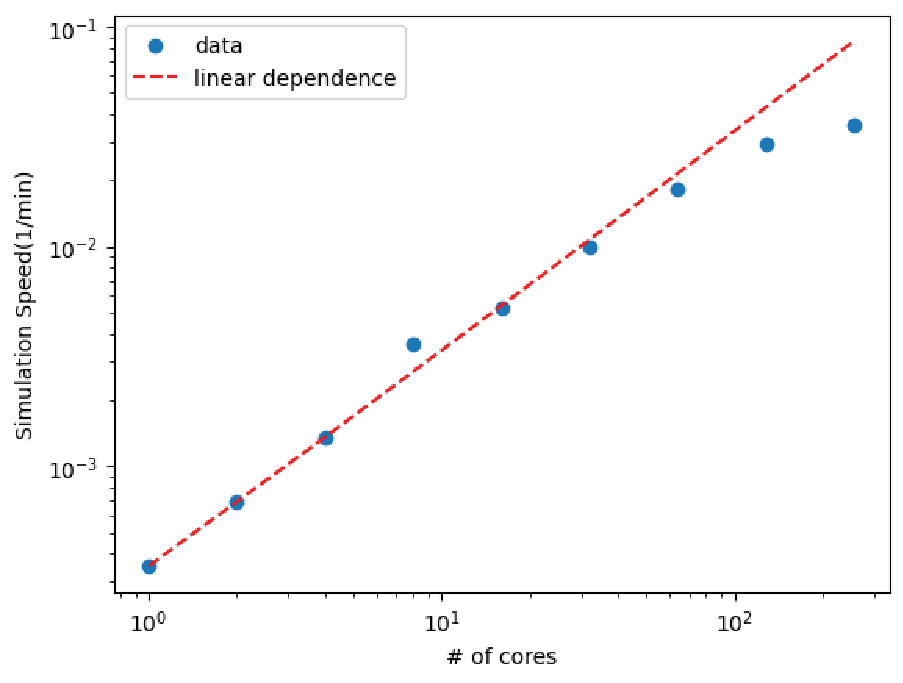
\includegraphics[width=\linewidth]{parallelPerf.pdf}
\caption[Performance of openmd\_MPI on parallel machines]{The
  parallel implementation of OpenMD yields linear speedup up to
  approximately 50 cores on relatively modern machines. Note that
  system size and composition as well as cluster architecture have a
  large impact on this behavior.}
\label{fig:parallelPerf}
\end{figure}


There is one interesting issue with of how OpenMD distributes load on
parallel (MPI) architectures.  At the very beginning of a parallel
simulation, the molecules are distributed among the processors using a
short Monte Carlo procedure to divide the labor.  This ensures that
each processor has an approximately equal number of atoms to work
with, and that the row- and column-distribution of atoms in the force
decomposition is roughly equitable. The Monte Carlo procedure
involves the use of a pseudo-random number to make processor
assignments. So, if you run the same parallel simulation multiple
times, the distribution of atoms on the processors can change from run
to run.

One thing that many people forget is a specific limitation of floating
point arithmetic.  Due to roundoff errors, the associative laws of
algebra do not necessarily hold for floating-point numbers. For
example, on a computer, the sum
\begin{equation*}
(x+y)+z
\end{equation*}
can have a different answer than
\begin{equation*}
x+(y+z)
\end{equation*}
when $x = 10^{30}$, $y = -10^{30}$ and $z = 1$.  In the first case,
the answer we get is 1, while roundoff might give us 0 for the second
expression.  The addition-ordering roundoff issue can have effects on
a simulation that are somewhat subtle.  If you add up the forces on an
atom in a different order, the total force might change by a small
amount (perhaps 1 part in $10^{10}$). When we use this force to move that
atom, we’ll be off by a small amount (perhaps 1 part in $10^9$). These
small errors can start to make real differences in the {\it microstate} of a
simulation (i.e. the configuration of the atoms), but shouldn’t alter
the {\it macrostate} (i.e. the temperature, pressure, etc.).

That said, whenever there’s a random element to the order in which
quantities are added up, we can get simulations that are not
reproducible.  And non-reproducibility is, in general, not good.  So,
how do we get around this issue in OpenMD?  We let the user introduce
a static seed for the random number generator that ensures that we
always start with exactly the same set of pseudo-random numbers.  If
we seed the random number generator, then on the same number of
processors, we’ll always get the same division of atoms, and we’ll get
reproducible simulations.

To use this feature simply add a seed value to your {\tt <MetaData>} section:

{\tt seed = 8675309;}

This seed can be any large positive integer (an {\tt unsigned long int}).

Once the seed is set, you can run on MPI clusters and be reasonably
sure of getting reproducible simulations for runs with the same number
of processors.  However, if you mix runs of different numbers of
processors, then the roundoff issue will reappear.
 
\chapter{\label{section:conclusion}Conclusion}

We have presented a new parallel simulation program called 
OpenMD. This program offers some novel capabilities, but mostly makes
available a library of modern object-oriented code for the scientific
community to use freely.  Notably, OpenMD can handle symplectic
integration of objects (atoms and rigid bodies) which have
orientational degrees of freedom.  It can also work with transition
metal force fields and point-dipoles. It is capable of scaling across
multiple processors through the use of force based decomposition. It
also implements several advanced integrators allowing the end user
control over temperature and pressure. In addition, it is capable of
integrating constrained dynamics through both the RATTLE
algorithm and the $z$-constraint method.

We encourage other researchers to download and apply this program to
their own research problems.  By making the code available, we hope to
encourage other researchers to contribute their own code and make it a
more powerful package for everyone in the molecular dynamics community
to use.  All source code for OpenMD is available for download at
{\tt http://openmd.org}.

\chapter{Acknowledgments}

Development of OpenMD was funded by a New Faculty Award from the
Camille and Henry Dreyfus Foundation and by the National Science
Foundation under grants CHE-0134881, CHE-0848243, CHE-1362211,
CHE-1663773, and CHE-191954648. Computation time was provided by the
Notre Dame Center for Research Computing.

\bibliographystyle{unsrt}
\bibliography{openmdDoc}

\end{document}
